%%%%% - PREÁMBULO - %%%%%%%%%%%%%%%%% 

% ----------------- Documento ----------------- %
% Se define el tipo de documento (en este caso un libro), en hoja A4 con tamaño de fuente de 11pt, escrito en castellano, e indicando que el documento tendrá páginas distintas a izquierda y derecha ("twoside"). Los documentos de tipo "book" comienzan todos los capítulos por defecto en una página impar, para que los capítulos comiencen en cualquier página y no haya que incluir una página en blanco se deb insertar el comando "openany":
\documentclass[a4paper, 11pt, spanish, twoside, openright]{book}
% Los demás tipos de documentos así como sus características y opciones pueden consultarse en: https://en.wikibooks.org/wiki/LaTeX/Document_Structure#Document_classes
% ---------------------------------------------- %

\newcommand{\tildea}[1]{\overset{\sim}{#1}}
\newcommand{\linkrepositorio}{https://github.com/Miguel-LA/TFM_MiguelLerinAlonso}

% ------------------ Variables internas -------------------- %
% Una forma de trabajar con cadenas de texto que se repiten mucho a lo largo de todo el doc, es definir variables internas del mismo. En este caso creo una variable para el título del TFM, que lo incluya en todos los encabezados y pies de página. 
% Como esto está escrito en formarto "book" hay que modificar los encabezados de las páginas de inicio de capítulo, para no estar cambiando cuatro veces cuatro líneas siempre que se me ocurra un nuevo nombre para el TFM, lo hago así.
\newcommand\tituloTrabajo{Diseño, implementación y validación  de arquitectura en ROS2 para estación robotizada de fabricación aditiva}
% \newcommand\tituloTrabajo{DISEÑO, IMPLEMENTACIÓN Y VALIDACIÓN DE ARQUITECTURA EN ROS2 PARA ESTACIÓN ROBOTIZADA DE FABRICACIÓN ADITIVA}


% ------------------ Página -------------------- %
% Se define el tamaño de las páginas, indicando el tamaño de los márgenes superior e inferior ("top" y "bottom"), e izquierdo y derecho ("left" y "right"):
\usepackage[top=2.5cm,bottom=2.5cm,left=2.5cm,right=2.5cm]{geometry}
% Se inserta el comando \raggedbottom para evitar que LaTeX rellene con espacios en blanco aquellas páginas que no alberguen suficiente contenido como para rellenarlas de forma "natural":
\raggedbottom 
% ---------------------------------------------- %


% ------------- Paquetes generales ------------- %
% Se importan distintos paquetes de propósito general:
\usepackage[utf8]{inputenc}
\usepackage[spanish,es-tabla]{babel}
\usepackage{float}
\usepackage{caption}
% ---------------------------------------------- %


% ------------ Paquetes específicos ------------ %
% Se importan distintos paquetes que será utilizados en momentos concretos del documento: 
\usepackage{pdfpages} % Para insertar la portada en formato PDF.
\usepackage{amssymb} % Para símbolos matemáticos.
\usepackage{bm} % Para negrita en símbolos matemáticos.
\usepackage{amsmath} % Para el entorno "split".
\usepackage[hidelinks]{hyperref, bookmark} % Para urls.
\usepackage{longtable} % Para tablas largas.
\usepackage{tabularray} % Para tablas con celdas combinadas.
\usepackage{pgf} % Para gráficas en formato PGF.
\usepackage{graphicx} % Para insertar imágenes.
\usepackage{wrapfig} % Para posicionar imágenes alrededor del texto.
\usepackage{fontawesome5} % Para utilizar iconos de "fontawesome".
\usepackage{pdflscape}  % Para colocar páginas en formato apaisado.
\usepackage{adjustbox}
\usepackage[inkscapelatex=false]{svg}
\usepackage{nameref}
\usepackage{relsize}

\usepackage{graphicx}
\usepackage{eurosym}    % Para poner el símbolo del euro bonito

\usepackage{algorithm}  % Para introducir algoritmos en forma de pseudocódigo
\usepackage{algpseudocode}
\floatname{algorithm}{Algoritmo}
\renewcommand{\listalgorithmname}{Lista de algoritmos}
\renewcommand{\algorithmicrequire}{\textbf{Entrada:}}
\renewcommand{\algorithmicensure}{\textbf{Salida:}}
\renewcommand{\algorithmicend}{\textbf{fin}}
\renewcommand{\algorithmicif}{\textbf{si}}
\renewcommand{\algorithmicthen}{\textbf{entonces}}
\renewcommand{\algorithmicelse}{\textbf{si no}}
\renewcommand{\algorithmicelsif}{\textbf{y si no}}
\renewcommand{\algorithmicendif}{\textbf{fin si}}
\renewcommand{\algorithmicfor}{\textbf{para}}
\renewcommand{\algorithmicforall}{\textbf{para todo}}
\renewcommand{\algorithmicdo}{\textbf{hacer}}
\renewcommand{\algorithmicendfor}{\textbf{fin para}}
\renewcommand{\algorithmicwhile}{\textbf{mientras}}
\renewcommand{\algorithmicendwhile}{\algorithmicend\ \algorithmicwhile}
\renewcommand{\algorithmicloop}{\textbf{repetir}}
\renewcommand{\algorithmicendloop}{\algorithmicend\ \algorithmicloop}
\renewcommand{\algorithmicrepeat}{\textbf{repetir}}
\renewcommand{\algorithmicuntil}{\textbf{hasta que}}
\renewcommand{\algorithmicprint}{\textbf{imprimir}} 
\renewcommand{\algorithmicreturn}{\textbf{devolver}} 
\renewcommand{\algorithmictrue}{\textbf{cierto }} 
\renewcommand{\algorithmicfalse}{\textbf{falso }} 


% ---------------------------------------------- %


% ------------------ Parámetros del PDF -------------------- %
% Se indican los parámetros del PDF resultante como el nombre que aparece en el lector o las palabras clave para los metadatos.

\hypersetup{
    pdftitle={Miguel Lerín Alonso - TFM - 2024},
    pdfsubject={TFM - 2024},
    pdfauthor={Miguel Lerín Alonso},
    pdfkeywords={Extrinsic calibration, hybrid learning, intrinsic calibration, manufacturing station, non-planar additive manufacturing, offline learning, online learning, robotic addtive manufacturing, ROS2 enviroment},
    colorlinks,
    citecolor=blue,
    filecolor=black,
    linkcolor=black,
    urlcolor=black,
}
% ---------------------------------------------- %


% ---------------- Numeración ------------------ %
\counterwithin{table}{chapter} % Se numeran las tablas con respecto al capítulo en el que se encuentran.
\counterwithin{figure}{chapter} % Se numeran las figuras con respecto al capítulo en el que se encuentran.
\counterwithin{equation}{chapter} % Se numeran las ecuaciones con respecto al capítulo en el que se encuentran.
% ---------------------------------------------- %

% ------------- Página en blanco ----------------%
% Se define un comando (\blankpage) para insertar una página totalmente en blanco (sin número de página, encabezado y pie de página):
\usepackage{afterpage}
\newcommand\blankpage{%
    \null
    \thispagestyle{empty}%
    \newpage}
% ---------------------------------------------- %    


% ----------- Formato de los párrafos -----------%
% Se define el formato de los párrafos:
\setlength{\parindent}{0pt} % Se elimina la sangría en comienzo de párrafo (0pt).
\setlength{\parskip}{1em} % Se define el espacio entre dos párrafos (1em).
% ---------------------------------------------- %    


% -------------- Título adicional -------------- %
% Se añade una profundidad adicional a los títulos (profundidad 4):
\usepackage{titlesec}
\setcounter{secnumdepth}{4} % Se fija en 4 la profundidad de numeración de títulos.
\setcounter{tocdepth}{4} % Se fija en 4 la profundidad de títulos incluidos en el índice.
% Se modifica el formato de \paragraph (título de profundidad 4) para adaptarlo al formato del resto de títulos:
\titleformat{\paragraph}
{\normalfont\normalsize\bfseries}{\theparagraph}{1em}{}
\titlespacing*{\paragraph}
{0pt}{3.25ex plus 1ex minus .2ex}{1.5ex plus .2ex} 
% ---------------------------------------------- %    


% --------- Encabezado y pie de página -------- %
% El encabezado y pie de página forman parte del paquete fancyhdr:
\usepackage{fancyhdr}
\fancyhf{}
\pagestyle{fancy}

% Se ajusta el tamaño de fuente para el encabezado y pie de página (9pt)
\fancyhf{\fontsize{2}{12}\selectfont}

% Contenido del encabezado (\fancyhead):
\fancyhead[RO]{\tituloTrabajo} % Texto que se coloca en el encabezado de las páginas impares (O -> 'Odd', o impar) a la izquierda (R -> 'Odd')

\renewcommand{\chaptermark}[1]{\markboth{#1}{}}
\fancyhead[LE]{\MakeUppercase{\leftmark}} % Texto que se coloca en el encabezado de las páginas pares (E -> 'Even', o par) a la izquierda (L -> 'Left'). \rightmark se utiliza para insertar automáticamente el título de la sección correspondiente, y \nouppercase para que no aparezca todo en mayúsculas (formato por defecto de \rightmark). Si usas el tipo de documento "book" para que aparezca el título del capítulo dbes cambiar rightmark por leftmark, pero antes debes introducir la línea de código \renewcommand{\chaptermark}[1]{\markboth{#1}{}} para que sólo te aparezca el título del capítulo (para más info consultar pág. 19 de http://tug.ctan.org/tex-archive/macros/latex/contrib/fancyhdr/fancyhdr.pdf).

% Contenido del pie de página (\fancyfoot):
\fancyfoot[RE]{Escuela  Técnica  Superior  de  Ingenieros  Industriales  (UPM)} % Texto que se coloca en el pie de página de las páginas pares (E -> 'Even', o par) a la derecha (R -> 'Right')
\fancyfoot[LO]{Miguel Lerín Alonso} % Texto que se coloca en el pie de página de las páginas impares (O -> 'Odd', o impar) a la izquierda (L -> 'Left')
\fancyfoot[LE,RO]{\thepage} % El número de página (\thepage) se coloca a la izquierda en las páginas pares y a la derecha en las impares.

% Se indica que sólo se quiere incorporar en \rightmark (utilizado más arriba) el título de la sección (y no de las subsecciones, subsubsecciones, etc.):
\renewcommand{\sectionmark}[1]{\markright{\thesection. #1}}
\renewcommand{\subsectionmark}[1]{}

% Formato de la línea de separación horizontal:
\renewcommand{\headrulewidth}{0.5pt} % Ancho de la línea del encabezado.
\renewcommand{\footrulewidth}{0.5pt} % Ancho de la línea del pie de página.

%% Cuando usamos el tipo de documento "book" los encabezados y pies de página de los comienzos del cada cap, van a su bola. utilizan directamente el estilo "plain". la mejor solución es modificar el estilo plain, se aplicará solamente al comenzar el capítulo y se puede hacer para que coincida con el normal.
\fancypagestyle{plain}{
\fancyhead[RO]{\tituloTrabajo} 
\fancyhead[LE]{\tituloTrabajo} 
\fancyfoot[RE]{Escuela  Técnica  Superior  de  Ingenieros  Industriales  (UPM)}
\fancyfoot[LO]{Miguel Lerín Alonso}
\fancyfoot[LE,RO]{\thepage}}
% ---------------------------------------------- % 

  
% -------------- Diagramas TikZ ---------------- %
% Se importa el paquete TikZ para diagramas de propósito general (diagramas de bloques, de flujo, etc.):
\usepackage{tikz}
\usetikzlibrary{shadows, trees, shapes.geometric}
\tikzset{
every picture/.append style={
  execute at begin picture={\deactivatequoting},
  execute at end picture={\activatequoting}
  }
}
% Se importa el paquete circuitikz para circuitos eléctricos:
\usepackage{circuitikz}
% ---------------------------------------------- % 


% ----------- Fragmentos de código ------------- %
% El paquete utilizado para insertar fragmentos de código en el documento es listings. En el presente bloque del preámbulo se definen ciertos parámetros de listings con el objetivo de adaptar dicho paquete a código escrito en Python.

\usepackage{listings} % Paquete para insertar código. 
\usepackage{xcolor} % Paquete para definir colores.

% Se definen los distintos colores que se utilizan para resaltar ciertos elementos del código:
\definecolor{codegreen}{rgb}{0.04314,0.6745,0.07843} % Verde.
\definecolor{codegray}{rgb}{0.5,0.5,0.5} % Gris.
\definecolor{codered}{rgb}{0.5373,0.02745,0.06275} % Rojo.
\definecolor{codeblue}{rgb}{0.071,0.0258,0.9882} % Azul.
\definecolor{codepurple}{rgb}{0.6,0.02745,0.5961} % Morado.

% Se define el color de fondo:
\definecolor{backcolour}{rgb}{0.95,0.95,0.92} % Gris oscuro.

% Se define el valor de ciertos parámetros de listings para adaptar dicho paquete a código escrito en Python:
\lstdefinestyle{mystyle}{
    % - General:
    language=Python, % Lenguaje de programación.
    basicstyle=\ttfamily\footnotesize, % Tipografía y tamaño de fuente.
    % - Colores de los distintos elementos del código:
    backgroundcolor=\color{backcolour}, % Color de fondo.  
    commentstyle=\color{codegray}, % Color de los comentarios.
    keywordstyle=\color{codeblue}, % Color de las palabras clave por defecto.
    stringstyle=\color{codegreen}, % Color de los "string"
    % - Palabras clave:
    deletekeywords={print}, % Se elimina "print" del conjunto de palabras clave para posteriormente asignarle el color morado.
    keywordstyle={[2]\ttfamily\color{codeblue}},
    keywords=[2]{as}, % Se añaden las palabras clave de color azul.
    keywordstyle={[3]\ttfamily\color{codepurple}},
    keywords=[3]{True, False, ttk, list, None, dict, zip, range, len, print, float, sum}, % Se añaden las palabras clave de color morado.
    keywordstyle={[4]\bfseries\ttfamily},
    keywords=[4]{_read_excel}, % Se añaden las palabras clave en negrita.
    emph={MyClass,__init__}, % Se añaden las palabras clave enfatizadas.   
    % - Números de línea:
    numberstyle=\tiny\color{codegray}, % Tamaño de fuente y color de los números de línea.
    numbers=left, % Se colocan los números de línea en el lado izquierdo.                 
    numbersep=5pt, % Separación horizontal de los números de línea.
    % - Saltos a la línea, espacios, indentación:
    breaklines=true, % Permitir saltos a la línea. 
    breakatwhitespace=true, % Saltar a la línea únicamente al encontrar espacios.
    postbreak = \mbox{{$\hookrightarrow$}\space}, % Se añade una flecha al cambiar de línea.
    showspaces=false, % No mostrar los espacios. 
    showstringspaces=false, % No mostrar los espacios en los "string".
    keepspaces=true, % Mantener los espacios presentes en el código. 
    tabsize=2, % Tamaño de indentación.
    % - Título:
    captionpos=b % Posición del título del fragmento de código (b=bottom - abajo).
} 
\lstset{style=mystyle} % Se asocia el estilo de listings al estilo que acaba de definirse ("mystyle")

% Se realizan una serie de operaciones complementarias con el paquete listings (su comprensión no es necesaria para manejar dicho paquete):
\makeatletter
\def\lst@OpLiteratekey#1\@nil@{\let\lst@ifxopliterate\lst@if
                             \def\lst@opliterate{#1}}
\lst@Key{opliterate}{}{\@ifstar{\lst@true \lst@OpLiteratekey}
                             {\lst@false\lst@OpLiteratekey}#1\@nil@}
\lst@AddToHook{SelectCharTable}
    {\ifx\lst@opliterate\@empty\else
         \expandafter\lst@OpLiterate\lst@opliterate{}\relax\z@
     \fi}
\def\lst@OpLiterate#1#2#3{%
    \ifx\relax#2\@empty\else
        \lst@CArgX #1\relax\lst@CDef
            {}
            {\let\lst@next\@empty
             \lst@ifxopliterate
                \lst@ifmode \let\lst@next\lst@CArgEmpty \fi
             \fi
             \ifx\lst@next\@empty
                 \ifx\lst@OutputBox\@gobble\else
                   \lst@XPrintToken \let\lst@scanmode\lst@scan@m
                   \lst@token{#2}\lst@length#3\relax
                   \lst@XPrintToken
                 \fi
                 \let\lst@next\lst@CArgEmptyGobble
             \fi
             \lst@next}%
            \@empty
        \expandafter\lst@OpLiterate
    \fi}

\lstset{ 
    literate={á}{{\'a}}1 {é}{{\'e}}1 {í}{{\'i}}1 {ó}{{\'o}}1 {ú}{{\'u}}1
  {Á}{{\'A}}1 {É}{{\'E}}1 {Í}{{\'I}}1 {Ó}{{\'O}}1 {Ú}{{\'U}}1
  {à}{{\`a}}1 {è}{{\`e}}1 {ì}{{\`i}}1 {ò}{{\`o}}1 {ù}{{\`u}}1
  {À}{{\`A}}1 {È}{{\'E}}1 {Ì}{{\`I}}1 {Ò}{{\`O}}1 {Ù}{{\`U}}1
  {ä}{{\"a}}1 {ë}{{\"e}}1 {ï}{{\"i}}1 {ö}{{\"o}}1 {ü}{{\"u}}1
  {Ä}{{\"A}}1 {Ë}{{\"E}}1 {Ï}{{\"I}}1 {Ö}{{\"O}}1 {Ü}{{\"U}}1
  {â}{{\^a}}1 {ê}{{\^e}}1 {î}{{\^i}}1 {ô}{{\^o}}1 {û}{{\^u}}1
  {Â}{{\^A}}1 {Ê}{{\^E}}1 {Î}{{\^I}}1 {Ô}{{\^O}}1 {Û}{{\^U}}1
  {Ã}{{\~A}}1 {ã}{{\~a}}1 {Õ}{{\~O}}1 {õ}{{\~o}}1
  {œ}{{\oe}}1 {Œ}{{\OE}}1 {æ}{{\ae}}1 {Æ}{{\AE}}1 {ß}{{\ss}}1
  {ű}{{\H{u}}}1 {Ű}{{\H{U}}}1 {ő}{{\H{o}}}1 {Ő}{{\H{O}}}1
  {ç}{{\c c}}1 {Ç}{{\c C}}1 {ø}{{\o}}1 {å}{{\r a}}1 {Å}{{\r A}}1
  {€}{{\euro}}1 {£}{{\pounds}}1 {«}{{\guillemotleft}}1
  {»}{{\guillemotright}}1 {ñ}{{\~n}}1 {Ñ}{{\~N}}1 {¿}{{?`}}1
  {º}{{\textordmasculine}}1}

\lstset{opliterate=
   *{0}{{{\color{codered}0}}}1 {1}{{{\color{codered}1}}}1 
   {2}{{{\color{codered}2}}}1 {3}{{{\color{codered}3}}}1 
   {4}{{{\color{codered}4}}}1 {5}{{{\color{codered}5}}}1 
   {6}{{{\color{codered}6}}}1 {7}{{{\color{codered}7}}}1 
   {8}{{{\color{codered}8}}}1 {9}{{{\color{codered}9}}}1}

\DeclareCaptionType{code}[Código][ÍNDICE DE CÓDIGOS] % Se define el entorno "Código" (de forma que al introducir un fragmento de código en el documento aparezca como: Código 1.1: ...), y la lista con los distintos códigos ("Índice de códigos").
\counterwithin{code}{section} % Se numeran los códigos con respecto al capítulo en el que se encuentran.
% ---------------------------------------------- % 


% --------------- Bibliografía ----------------- %
% El manejo de la bibliografía se realiza mediante el paquete biblatex:
\usepackage[backend=biber, style=ieee, sorting=none, citestyle=ieee, maxcitenames=2, mincitenames=1, maxbibnames=5, giveninits=true, uniquename=init]{biblatex} 

%  Para poner el número de las citas en color azul se usa el paquete hyperef y luego se especifica el color del número en inglés. Se puede hacer lo mismo con el color de las referencias internas y las url insertadas.
\hypersetup{
  colorlinks=true,
  citecolor=blue,
  linkcolor=false,
  urlcolor=false,
  }

% Los distintos parámetros que aparecen en la línea anterior corresponden a las siguientes características de la bibliografía:
% - style: la manera en la que aparecen las referencias en la bibliografía. En este caso se opta por "authoryear", pero existen múltiples estilos posibles que se resumen en la siguiente guía: https://www.overleaf.com/learn/latex/biblatex_bibliography_styles.
% - sorting: orden en el que aparecen las distintas referencias en la bibliografía. En este caso se opta por ordenarlas en primer lugar por el apellido del primer autor, en segundo lugar por el año de publicación, y por último por el título de la publicación (nyt=name-year-title)
% - citestyle: elementos y orden de dichos elementos de una referencia al citarla en el documento. En este caso se escoge "authoryear" para que aparezca en primer lugar el apellido del autor (o de los autores) y en segundo lugar el año de publicación. Existe gran variedad de opciones en cuanto al parámetro citestyle que se resumen en: https://www.overleaf.com/learn/latex/biblatex_citation_styles.
% maxcitenames: máximo número de autores que aparecen al citar una referencia en el documento. Al escoger un valor de 2 para este parámetro se pueden dar los siguientes casos: un único autor -> (autor, año), dos autores -> (autor 1 y/e autor 2, año), tres o más autores -> (autor 1 et al., año).
% maxbibnames: parámetro idéntico al anterior pero para la bibliografía en lugar de las citas.
% giveinits y uniquename: para mostrar únicamente las iniciales de los nombres de los autores.

% Se importa el paquete csquotes para citar las referencias a lo largo del documento:
\usepackage{csquotes} 

% Se realizan una serie de operaciones para adaptar la bibliografía al estilo deseado (coma entre autor y año al citar una referencia, idioma castellano, etc.):
\DeclareNameAlias{sortname}{family-given}
\renewcommand*{\nameyeardelim}{\addcomma\space}
\setlength\bibitemsep{\baselineskip}
\DefineBibliographyStrings{spanish}{%
  andothers = {et\addabbrvspace al\adddot}
}

\makeatletter

\newrobustcmd*{\parentexttrack}[1]{%
  \begingroup
  \blx@blxinit
  \blx@setsfcodes
  \blx@bibopenparen#1\blx@bibcloseparen
  \endgroup}

\AtEveryCite{%
  \let\parentext=\parentexttrack%
  \let\bibopenparen=\bibopenbracket%
  \let\bibcloseparen=\bibclosebracket}

\makeatother

\addbibresource{bibliografia/biblio.bib}
% ---------------------------------------------- % 


% --------------- Anexos y apéndices ----------------- %
\usepackage{appendix}

\renewcommand{\appendixname}{APÉNDICE}
\renewcommand{\appendixtocname}{APÉNDICES}
\renewcommand{\appendixpagename}{APÉNDICES}
% ---------------------------------------------- % 

% --------------- Siglas y acrónimos----------------- %
%% Hay que trabajar con dos ficheros .tex. En uno se lamacenan todas las siglas "glassy-entries.tex". Y en otro se maqueta el folio para que aparezca como un índice más "siglas_acronimos.tex", este último se debe poner al comenzar el documento.

\usepackage[acronyms, section=section]{glossaries}
\newacronym{AM}{AM}{Fabricación Aditiva (\textit{Additive Manufacturing})}
\newacronym{CAD}{CAD}{Diseño Asistido por Ordenador (\textit{Computer Aided Design})}
\newacronym{NPAM}{NPAM}{Fabricación Aditiva No Planar (\textit{Non Planar Additive Manufacturing})}
\newacronym{CNC}{CNC}{Control Numérico por Computador}
\newacronym{SM}{SM}{Fabricación Sustractiva (Substractive Manufacturing)}
%% \newacronym{UV}{UV}{Luz Ultra Violeta}
\newacronym{SLA}{SLA}{Estereolitografía}
\newacronym{MEX}{MEX}{Extrusión de material (\textit{Material Extrusion})}
\newacronym{ROS}{ROS}{Robotic Operating System}
\newacronym{OPAMP}{OPAMP}{Amplificador Operacional (\textit{Operational Amplifier})}
\newacronym{IGBT}{IGBT}{Transistor Bipolar de Puerta Aislada (\textit{Insulated Gate Bipolar Transistor})}
\newacronym{RX}{RX}{Rayos X}
\newacronym{MRI}{MRI}{Imagen de Resonancia Magnética (\textit{Magnetic Resonance Image})}
\newacronym{ABS}{ABS}{Acrilonitrilo Butadieno Estireno}
\newacronym{PLA}{PLA}{Ácido Poliláctico}
\newacronym{DOF}{DOF}{Grados de libertad (\textit{Degrees Of Freedom})}
\newacronym{STL}{STL}{STereoLithoraphy file}
\newacronym{LOM}{LOM}{Manufactura de Objeto Laminado (\textit{Laminated Object Manufacturing})}
\newacronym{LENS}{LENS}{Tejido de red Láser (\textit{Laser Engineered Net Shaping})}
\newacronym{SLS}{SLS}{Sinterizado Láser Selectivo (\textit{Selective Laser Sintering})}
\newacronym{SBC}{SBC}{Computador de placa única (\textit{Single Board Computer})}
\newacronym{TCP}{TCP}{Punto Central de Herramienta (\textit{Tool Center Point})}
\newacronym{TCP/IP}{TCP/IP}{Protocolo de control de transmisión/Protocolo de Internet (\textit{Transference Control Protocol/Internet Protocol})}
\newacronym{DDS}{DDS}{Servicio de distribución de datos (\textit{Data Distribution Service})}
\newacronym{YAML}{YAML}{YAML Ain't Markup Language}
\newacronym{URDF}{URDF}{Formato Unificado de Descripción del Robot (\textit{Unified Robot Description Format})}
\newacronym{VPP}{VPP}{Fotopolimerización en recipiente (\textit{Vat Photopolimerization})}
\newacronym{DED}{DED}{Deposición Directa de Energía (\textit{Direct Energy Deposition})}
\newacronym{AMF}{AMF}{Fichero de formato de fabricación aditiva (\textit{Additive Manufacturing File Format})}
\newacronym{DfAM}{DfAM}{Diseño para fabricación aditiva (\textit{Design for Additive Manufacturing})}
\newacronym{EDP}{EDP}{Estructura de Descomposición del Proyecto}
\newacronym{PLC}{PLC}{Computador lógico programable (\textit{Programmable Logic Computer})}
\newacronym{POO}{POO}{Programación Orientada a Objetos}



\makeglossaries
% ---------------------------------------------- % 

\usepackage{subcaption}

%%%%%%%%%%%% - INICIO DEL DOCUMENTO - %%%%%%%%%%%%

\begin{document} 

%%%%%%%%%%%%%%%%%%%%%%%%%%%%%%%%%%%%%%%%%%%%%%%%%%


%%%%%%%%%%%%%%%%%%% - PORTADA - %%%%%%%%%%%%%%%%%%

% Se comienza una página nueva sin formato (sin número de página y sin encabezado/pie de página), ya que sólo incorpora la la portada:
\newpage
\thispagestyle{empty}

% La portada se inserta mediante el comando \includepdf seguido del archivo PDF correspondiente (que se ajusta automáticamente a las dimensiones de la página):

% PORTADA HORIZONTAL (Toca girar el pdf)
% \begin{landscape}
%     \includepdf[angle=90]{portada_TFM_horizontal.pdf}
% \end{landscape}

% PORTADA VERTICAL
\includepdf{portada_TFM_vertical.pdf}


\blankpage

%%%%%%%%%%%%%%%%%%%%%%%%%%%%%%%%%%%%%%%%%%%%%%%%%%

% Las páginas anteriores al contenido del TFG/TFM (previas a la introducción) suelen numerarse de forma distinta a las del cuerpo del informe, en este caso en números romanos:
\pagenumbering{roman}

%%%%%%%%%%%%%%%%%%%%%%%%%%%%%%%%%%%%%%%%%%%%%%%%%%

%%%%%%%%%%%%%$%%%%% - PRESENTACIÓN GUAPISÍMA - %%%%%%%%%%%%%%%%%%%%%

\includepdf{hoja_presentacion_TFM.pdf}
\blankpage
%%%%%%%%%%%%%%%%%%%%%%%%%%%%%%%%%%%%%%%%%%%%%%%%%%


%%%%%%%%%%%%%$%%%%% - CITA - %%%%%%%%%%%%%%%%%%%%%
 
% Se comienza una página nueva sin formato (sin número de página y sin encabezado/pie de página), ya que sólo incorpora la cita:
\newpage
\thispagestyle{empty}

\begin{flushright} % Se alinea el texto en el lado derecho de la página.
\vspace*{5cm} % Se añade un espacio vertical de 5cm para situar la cita en ~1/3 de la página.

\textit{“Las circunstancias externas pueden despojarnos de todo, menos de una cosa: la libertad de elegir cómo responder a esas cicunstancias.”} 

\medskip % Salto a la línea de tamaño medio (existen \smallskip, \medskip y \bigskip)
- Viktor Frankl 

\end{flushright}

\afterpage{\blankpage} % Se añade una página en blanco después de la cita.

%%%%%%%%%%%%%%%%%%%%%%%%%%%%%%%%%%%%%%%%%%%%%%%%%%

%%%%%%%%%%%%% - AGRADECIMIENTOS - %%%%%%%%%%%%%%%%
% Se comienza una página nueva con formato plano (sin encabezado/pie de página pero con número de página):
\newpage
\thispagestyle{plain}

\chapter*{Agradecimientos} % Se añade un asterisco a \section para que el título no esté numerado.
%\addcontentsline{toc}{section}{Agradecimientos} % Al utilizar \section* se ha de añadir manualmente el apartado al índice (Table Of Contents, TOC).

A mis padres Elisa y Francisco por continuar a mi lado incondicionalmente. Siempre os estaré agradecido ensañarme el valor del sentido del deber, el tesón, el respeto por los demás y el no rendirme nunca.

A mi hermano Javier por enseñarme cada día que lo más importante es sonreír con la cabeza alta.

A mi familia. Por acompañarme siempre desde el primer momento y confiar en mí.

A mis amigos por ayudarme en el transcurso de mi carrera y mostrar interés en todos mis proyectos.

Por último y no menos importante, gracias mis tutores Daniel y Álvaro por todos los buenos momentos y frustraciones compartidas en el laboratorio. De vosotros he aprendido a buscar siempre a una ruta alternativa y a darle un giro nuevo a cada problema. También me llevo vuestro profundo interés por la ciencia y la labor docente.

\section*{Agradecimientos institucionales}
Doy las gracias al departamento de Ingeniería de Fabricación de la ETSII-UPM por la oportunidad ofrecida,  su interés en el proyecto y la forma de  trabajo que he podido aprender de ellos. Especialmente a Álvaro, Adrián y Enrique por el apoyo aportado, sea la situación que sea.

\vspace{1.5 cm}
A todos vosotros con todo lo que tengo, que es mi corazón, os digo sinceramente:

Gracias.

\afterpage{\blankpage} % Se añade una página en blanco después de los agradecimientos.

%%%%%%%%%%%%%%%%%%%%%%%%%%%%%%%%%%%%%%%%%%%%%%%%%%

%%%%%%%%%%%%%% - RESUMEN EJECUTIVO - %%%%%%%%%%%%%
\newpage

%%%%%% --- RESUMEN --- %%%%%
\pdfbookmark[section]{Resumen}{Resumen}
\chapter*{Resumen}  % Se añade un asterisco a \section para que el título no esté numerado.
\markright{Resumen} % Al utilizar \section* se ha de añadir manualmente el título del apartado al encabezado.
%\addcontentsline{toc}{chapter}{Resumen} % Al utilizar \section* se ha de añadir manualmente el apartado al índice (Table Of Contents, TOC).

Dentro del paradigma de la Industria 4.0, en concreto el referente a los sistemas de fabricación, las estaciones flexibles cada vez cobran una mayor relevancia. El creciente uso de este tipo de estaciones se ve impulsado por las necesidades de un mercado cada vez más exigente, en el que se favorece el empleo de componentes personalizados y rápidamente escalables.

La tecnología de fabricación aditiva supone una gran oportunidad por su capacidad para desarrollar multitud de diseños optimizando el material empleado y dotando al ingeniero responsable de una gran libertad en el diseño de sus piezas. Sin embargo, este tipo de tecnologías ve limitadas sus capacidades por dos aspectos cruciales para su evolución: la limitación de su volumen de trabajo y el bajo número de grados de libertad disponibles.

La primera se asocia a la necesidad de trabajar con piezas de tamaño reducido, lo que obliga al usuario a pensar en diseños por partes que se integren con facilidad en una estructura mayor. La segunda es la referente al difícil acceso que puede existir a los recovecos de las figuras de mayor complejidad. 

Como solución a estos problemas muchas empresas e investigadores han invertido grandes cantidades de dinero, tiempo y esfuerzo en el desarrollo de sistemas que integren un manipulador robótico de 6 grados de libertad. Es decir, se busca utilizar un elemento compacto de gran precisión y versatilidad en su espacio de movimiento.

El uso de este tipo de robots implica superar dos grandes problemáticas asociadas como son la generación de trayectorias complejas y la implementación del equipo dentro de un marco de comunicaciones de mayor nivel, donde pueda ser un elemento más de una estación de fabricación flexible. Esto es, que tenga capacidad para recibir y enviar mensajes provenientes de otros elementos de la planta industrial -como la red de comunicaciones inalámbricas, el sistema de aporte de material o los sensores asociados- mientras realiza automáticamente los movimientos asociados al proceso de fabricación.

En el presente proyecto, se propone e implementa un diseño de arquitectura de control automático para una estación de fabricación aditiva que integre este tipo de robot en un proceso que usa trayectorias de alta complejidad como la \acrfull{NPAM}. Este sistema se construye utilizando el entorno de software proporcionado por ROS2 para el cálculo de trayectorias no planares, que se han utilizado como marco de validación de la capacidad del sistema para el cálculo y trazado de trayectorias complejas.

El proyecto se ha desarrollado dentro del marco de trabajo que proporciona el entorno del departamento de \hyperlink{https://fabricacion.industriales.upm.es/}{Ingeniería de Fabricación} de la ETSII-UPM. Es un esfuerzo multidisciplinar en el que se ha efectuado una labor de coordinación entre varios equipos especialistas en campos como la automatización de procesos, la electrónica de control, la programación de algoritmos de laminado, diseño de producto o de instalaciones industriales.

El proyecto se ha desarrollado en cuatro pilares esenciales como son (1) el diseño de una arquitectura de control que satisfaga las necesidades de las diferentes disciplinas implicadas en la construcción de la estación, (2) el desarrollo de un sistema de lectura de datos provenientes del robot manipulador y los equipos conectados al mismo, (3) la definición y validación de un sistema de cálculo y ejecución de trayectorias a partir de modelos tridimensionales del entorno de trabajo y los productos deseados y (4) un sistema de calentamiento automático de uno de los elementos auxiliares al manipulador robótico como es la plataforma de impresión. Los cuatro pilares cuentan con un elemento común que sirve de nexo común para la comunicación, definición y ejecución de sus respectivas tareas: el entorno de programación robótica ROS2.

Estos cuatro pilares tienen su propia entidad y se enlazan sucesivamente en el diseño, implementación y validación de la estación, constituyendo cada uno su propio capítulo en el que se define un universo propio conformado por el problema que le corresponde, la metodología que se propone como solución y los resultados que aporta.

En líneas generales del proyecto, se dice que éste comienza con la definición del flujo de trabajo asociado al proceso aditivo no planar que se desea robotizar y la propuesta de arquitectura informática que puede implementarlo en la estación de fabricación. Posteriormente, se aborda la problemática de la obtención de información directa proveniente del manipulador robótico y el conjunto de sensores/actuadores conectados al mismo, con resultados positivos en cuanto a la integración rápida de una gran variedad de equipos y mensajes.

La etapa de mayor relevancia del proyecto es la referente al sistema de ejecución automática de trayectorias no planares, en la que se define un modelo de programación basado en ROS2 que permite combinar aportes de la filosofía de planificación de trayectorias offline y online. Este enfoque se basa en la integración de la calibración automática del manipulador con un entorno de cálculo automático de trayectorias basado en restricciones de espacio de trabajo, tiempo y velocidad de ejecución. Los resultados observados abren la puerta al desarrollo de nuevos sistemas de este tipo aunque hacen especial hincapié en la necesidad de un sistema común de definición de trayectorias no planares como entrada al algoritmo de cálculo cinemático de la estación.

De forma paralela se trabaja en la regulación automática de la temperatura alcanzada por la plataforma de impresión, que trabaja como un elemento relativamente independiente del robot industrial pero perteneciente a la estación de fabricación. Es decir, se pasa por definir un sistema de control dinámico de la temperatura de la plataforma que sea capaz de comunicar su estado al resto de la estación para que se gestionen adecuadamente el resto de operaciones definidas en el flujo de trabajo.

Todas las tareas planteadas han acabado realizándose con éxito y como cierre al proyecto se hace un balance de los resultados aportados por todos los sistemas y flujos de trabajo con los que se ha trabajado. En él se evalúan las mayores limitaciones observadas durante el trabajo realizado -las cuales pueden restringir el correcto funcionamiento de la plataforma de impresión- y se comenta el valor aportado por las soluciones adoptadas. También se dedica una sección a posibles mejoras de cara a futuros proyectos.

\textbf{Palabras clave:} Aprendizaje híbrido, aprendizaje offline, aprendizaje online, calibración extrínseca, calibración intrínseca, ecosistema ROS2, estación de fabricación, fabricación aditiva no planar, fabricación robotizada.

\section*{Códigos UNESCO} 
\begin{itemize}
    \item[] 12 - Matemáticas
        \begin{itemize}
            \item[] 1201 - Álgebra
            \item[] 1203 - Ciencias de la computación 
            \item[] 1204 - Geometría 
            \item[] 1206 - Análisis numérico
            \item[] 1207 - Investigación operativa
        \end{itemize}
        
    \item[] 22 - Física
        \begin{itemize}
            \item[] 2203 - Electrónica
            \item[] 2205 - Mecánica 
        \end{itemize}
        
    \item[] 33 - Ciencias tecnológicas
        \begin{itemize}
            \item[] 3304 - Tecnología de los ordenadores
            \item[] 3307 - Tecnología electrónica
            \item[] 3310 - Tecnología industrial
            \item[] 3311 - Instrumentación tecnológica
            \item[] 3313 - Tecnología e ingeniería mecánica
            \item[] 3325 - Tecnología de las telecomunicaciones
        \end{itemize}
\end{itemize}

%%%%%% --- ABSTRACT --- %%%%%
\newpage
\pdfbookmark[section]{Abstract}{Abstract}
\chapter*{Abstract}  % Se añade un asterisco a \section para que el título no esté numerado.
\markright{Abstract} % Al utilizar \section* se ha de añadir manualmente el título del apartado al encabezado.
%\addcontentsline{toc}{chapter}{Abstract} % Al utilizar \section* se ha de añadir manualmente el apartado al índice (Table Of Contents, TOC).

Within the paradigm of Industry 4.0, specifically regarding manufacturing systems, flexible stations are becoming increasingly significant. The growing use of such stations is driven by the needs of an ever-demanding market, which favors the use of personalized and rapidly scalable components.

Additive manufacturing technology presents a great opportunity due to its ability to develop a multitude of designs while optimizing the material used, providing the responsible engineer with significant freedom in the design of their parts. However, this type of technology is limited by two crucial aspects for its evolution: the limitation of its work volume and the low number of available degrees of freedom.

The first is associated with the need to work with small-sized parts, which forces the user to think in terms of designs that can be easily integrated into a larger structure. The second pertains to the difficult access that may exist to the recesses of more complex figures.

As a solution to these problems, many companies and researchers have invested large amounts of money, time, and effort in developing systems that integrate a robotic manipulator with 6 degrees of freedom. That is, the aim is to use a compact element with high precision and great versatility in its movement space.

The use of this type of robots involves overcoming two major associated problems: the generation of complex trajectories and the implementation of the equipment within a higher-level communication framework, where it can be an element of a flexible manufacturing station. That is, it must be able to receive and send messages from other elements of the industrial plant - such as the wireless communication network, the material supply system, or associated sensors - while automatically performing the movements associated with the manufacturing process.

In the present project, an automatic control architecture design for an additive manufacturing station is proposed and implemented, integrating this type of robot in a process that uses high-complexity trajectories such as \acrfull{NPAM}. This system is built using the software environment provided by ROS2 for the calculation of non-planar trajectories, which have been used as a validation framework for the system's capability to calculate and trace complex trajectories.

The project has been developed within the framework provided by the environment of the \hyperlink{https://fabricacion.industriales.upm.es/}{Manufacturing Engineering} department of ETSII-UPM. It is a multidisciplinary project in which coordination work has been carried out between several teams specializing in fields such as process automation, control electronics, programming slicing algorithms, product design, or industrial installations.

The project has been developed on four essential pillars: (1) the design of a control architecture that meets the needs of the different disciplines involved in the construction of the station, (2) the development of a data reading system from the robotic manipulator and the connected equipment, (3) the definition and validation of a trajectory calculation and execution system based on three-dimensional models of the work environment and desired products, and (4) an automatic heating system for one of the auxiliary elements to the robotic manipulator, such as the printing platform. The four pillars share a common element that serves as a link for the communication, definition, and execution of their respective tasks: the ROS2 robotic programming environment.

These four pillars have their own entity and are successively linked in the design, implementation, and validation of the station, each constituting its own chapter in which a universe is defined by the corresponding problem, the proposed methodology as a solution, and the results provided.

In general terms of the project, it begins with the definition of the workflow associated with the non-planar additive process to be robotized and the proposal of the computing architecture that can implement it in the manufacturing station. Subsequently, the problem of obtaining direct information from the robotic manipulator and the set of connected sensors/actuators is addressed, with positive results in terms of the rapid integration of a wide variety of equipment and messages.

The most relevant stage of the project is related to the automatic execution system of non-planar trajectories, in which a programming model based on ROS2 is defined, allowing the combination of contributions from the offline and online trajectory planning philosophy. This approach is based on the integration of automatic manipulator calibration with an automatic trajectory calculation environment based on workspace, time, and execution speed constraints. The observed results pave the way for the development of new systems of this type, although they especially emphasize the need for a common system for defining non-planar trajectories as input to the kinematic calculation algorithm of the station.

In parallel, work is done on the automatic regulation of the temperature reached by the printing platform, which functions as a relatively independent element of the industrial robot but belongs to the manufacturing station. That is, a dynamic temperature control system for the platform is defined, capable of communicating its status to the rest of the station to manage the rest of the operations defined in the workflow appropriately.

All the tasks proposed have been successfully completed, and as a project closure, a balance of the results provided by all the systems and workflows worked on is made. It evaluates the major limitations observed during the work performed - which may restrict the proper functioning of the printing platform - and comments on the value provided by the adopted solutions. A section is also dedicated to possible improvements for future projects.

\textbf{Keywords:} Extrinsic calibration, hybrid learning, intrinsic calibration, manufacturing station, non-planar additive manufacturing, offline learning, online learning, robotic additive manufacturing, ROS2 enviroment


\section*{UNESCO Codes} 
\begin{itemize}
    \item[] 12 - Mathematics
        \begin{itemize}
            \item[] 1201 - Algebra
            \item[] 1203 - Computer Science
            \item[] 1204 - Geometry
            \item[] 1206 - Numerical Analysis
            \item[] 1207 - Operations Research
        \end{itemize}
        
    \item[] 22 - Physics
        \begin{itemize}
            \item[] 2203 - Electronics
            \item[] 2205 - Mechanics
        \end{itemize}
        
    \item[] 33 - Technological Sciences
        \begin{itemize}
            \item[] 3304 - Computer Technology
            \item[] 3307 - Electronic Technology
            \item[] 3310 - Industrial Technology
            \item[] 3311 - Instrumentation Technology
            \item[] 3313 - Mechanical Engineering and Technology
            \item[] 3325 - Telecommunications Technology
        \end{itemize}
\end{itemize}


% \afterpage{\blankpage} % Se añade una página en blanco después del resumen.
%%%%%%%%%%%%%%%%%%%%%%%%%%%%%%%%%%%%%%%%%%%%%%%%%%
\pdfbookmark[section]{ÍNDICES}{toc}
\chapter*{\centering ÍNDICES} \label{cap:indices}

%%%%%%%%%%%%%%%%%%% - ÍNDICE - %%%%%%%%%%%%%%%%%%%
%%\newpage
\pdfbookmark[subsection]{ÍNDICE GENERAL}{toc}
\renewcommand*\contentsname{ÍNDICE GENERAL} % Se modifica el nombre por defecto de la "Table Of Contents" (tabla de contenidos, índice) para pasar a llamarla "ÍNDICE DE CONTENIDO".
\tableofcontents % Se genera el índice de contenidos del documento que incorpora todos los títulos de \section, \subsection y \subsubsection (y también \paragraph, ver capítulo 1), así como los títulos añadidos con \addcontentsline (como el resumen ejecutivo, por ejemplo).
%%\afterpage{\blankpage} % Se añade una página en blanco después del índice.
%%%%%%%%%%%%%%%%%%%%%%%%%%%%%%%%%%%%%%%%%%%%%%%%%%

%%%%%%%%%%%%%% - ÍNDICE DE TABLAS - %%%%%%%%%%%%%%
\newpage
\renewcommand{\listtablename}{ÍNDICE DE TABLAS} % Se define el nombre del índice de tablas.
\pdfbookmark[subsection]{ÍNDICE DE TABLAS}{lot}
\listoftables % Se genera automáticamente el índice con las distintas tablas del documento (entorno \table o \longtable).
%\addcontentsline{toc}{section}{ÍNDICE DE TABLAS} % Se añade manualmente el apartado al índice (Table Of Contents, TOC).
%%%%%%%%%%%%%%%%%%%%%%%%%%%%%%%%%%%%%%%%%%%%%%%%%%


%%%%%%%%%%%%% - ÍNDICE DE FIGURAS - %%%%%%%%%%%%%%
\newpage
\renewcommand{\listfigurename}{ÍNDICE DE FIGURAS} % Se define el nombre del índice de figuras.
\pdfbookmark[subsection]{ÍNDICE DE FIGURAS}{lof}
\listoffigures % Se genera automáticamente el índice con las distintas figuras del documento (entorno \figure).
%\addcontentsline{toc}{section}{ÍNDICE DE FIGURAS} % Se añade manualmente el apartado al índice (Table Of Contents, TOC).
%%%%%%%%%%%%%%%%%%%%%%%%%%%%%%%%%%%%%%%%%%%%%%%%%%


%%%%%%%%%%%%%% - ÍNDICE DE ALGORITMOS - %%%%%%%%%%%%%
\newpage
\renewcommand{\listalgorithmname}{ÍNDICE DE ALGORITMOS}
\pdfbookmark[subsection]{ÍNDICE DE ALGORITMOS}{loc}
\listofalgorithms  % Se genera automáticamente el índice con los distintos códigos del documento (entorno \code).
%\addcontentsline{toc}{section}{ÍNDICE DE CÓDIGOS} % Se añade manualmente el apartado al índice (Table Of Contents, TOC).
%%%%%%%%%%%%%%%%%%%%%%%%%%%%%%%%%%%%%%%%%%%%%%%%%%


%%%%%%%%%%%%%% - ÍNDICE DE ABREVIATURAS - %%%%%%%%%%%%%
\pdfbookmark[subsection]{ÍNDICE DE ABREVIATURAS}{gls}
\chapter*{ÍNDICE DE ABREVIATURAS} \label{cap: siglas_acronimos}
\printglossary[title=, type=\acronymtype, nonumberlist]
%%%%%%%%%%%%%%%%%%%%%%%%%%%%%%%%%%%%%%%%%%%%%%%%%%
% \afterpage{\blankpage} % Se añade una página en blanco después del índice de códigos.


%%%%%%%%%%%%%%%%%%%%%%%%%%%%%%%%%%%%%%%%%%%%%%%%%%
% Se inicia una nueva página, y se restablece la numeración de las páginas, utilizando esta vez el sistema de numeración estándar (1, 2, 3, 4, ...)
\newpage
\pagenumbering{arabic}
%%%%%%%%%%%%%%%%%%%%%%%%%%%%%%%%%%%%%%%%%%%%%%%%%%


%%%%%%%%%%%%%%%%%%% - CAPÍTULOS DEL TRABAJO - %%%%%%%%%%%%%%%%%%
\chapter{Introducción} \label{cap: introduccion}

Este capítulo se plantea como una introducción al presente proyecto y su campo de estudio: la fabricación aditiva (\acrshort{AM}). El capítulo se encuentra dividido en cuatro bloques fundamentales. El primer bloque está destinado a la definición de los procesos \acrshort{AM} comentando su origen y sus aplicaciones más innovadoras.

El segundo bloque corresponde al estado del arte y se encuentra dividido en tres secciones: la primera será la responsable de describir el flujo de trabajo general seguido por los procesos de fabricación aditiva más convencionales, la segunda sección introducirá los sistemas \acrshort{AM} robotizados presentando las tecnologías de mayor impacto y dando unas pinceladas sobre la labor de preparación de estaciones. Finalmente, la tercera sección se centrará de forma específica en los procesos \acrshort{NPAM}.

A partir de lo presentado en el estado del arte, el tercer bloque indicará las limitaciones encontradas en el estado del arte y servirá para definir la motivación del proyecto. Esta reflexión servirá para introducir el cuarto y último bloque dedicado a la presentación del marco de proyecto dentro del departamento de \hyperlink{https://fabricacion.industriales.upm.es/}{Ingeniería de Fabricación} de la ETSII-UPM.

\section{Fabricación aditiva}
La \acrfull{AM} es un conjunto de procesos de fabricación enfocados en la producción de componentes tridimensionales a partir de un diseño \acrshort{CAD} previo y la adición de capas de material sobre diferentes soportes. La fabricación aditiva supone un campo novedoso en el que se dispone de una mayor libertad de diseño. Es decir, no existen las limitaciones de otras de técnicas de fabricación que suelen emplear procesos de eliminación de material (conocidos en literatura como \acrfull{SM}).

Los procesos de fabricación sustractiva se caracterizan por crear un producto final retirando material del bloque. En ellos se busca obtener la pieza en el menor tiempo posible, con coste reducido, tolerancias dimensionales ajustadas y especificaciones de diseño fijadas de antemano. Durante mucho tiempo estos procesos han sido la piedra angular de la industria manufacturera, siendo la opción  preferida para procesos a gran escala. Sin embargo, la retirada de material trae problemas de cara al prototipado y al ensayo de ciertas geometrías. La posibilidad de ahorrar los costes asociados a este tipo de operaciones ha servido como puerta de entrada de la \acrshort{AM} a sectores de mayor escala.

\begin{figure}[h!]
    \centering
    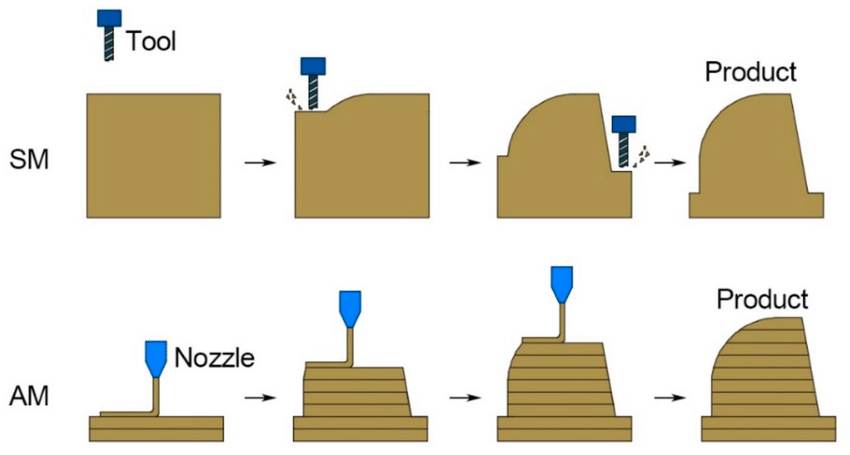
\includegraphics[scale=0.25]{figuras/sm_vs_am.png}
    \caption{Fabricación aditiva frente a sustractiva \cite{Tao2021}}
    \label{fig:aditiva_vs_sustractiva}
\end{figure}

Las técnicas de \acrshort{AM}, son idóneas para el desarrollo de piezas más personalizadas, la optimización de material, la reducción de residuos o la construcción de diseños de alta precisión y con geometrías complejas \cite{Li_2020} \cite{Rashid_2024}\cite{Loyda_2023}. No obstante, estos procesos son más lentos al requerir de métodos posteriores de limpieza, curado y acabado \cite{AMvsSM_Dasult}. En la figura \ref{fig:aditiva_vs_sustractiva} se muestra esquemáticamente el enfoque que aborda cada método de fabricación para una misma geometría. 

\subsection{Historia de la fabricación aditiva}
Los primeros registros de técnicas de fabricación aditiva son gracias al japonés Hideo Kodama, del Instituto Municipal de Investigación Industrial de Nagoya. En su trabajo publicado en 1981 \cite{Kodama1981}, Kodama habla de sus experimentos realizados con una resina fotosensible. Dicha resina se solidificaba en regiones concretas de un \textit{plotter} XY con ayuda de una matriz de haces de luz ultravioleta. Kodama pudo describir esta nueva tecnología con hasta tres métodos diferentes, los cuales se muestran la Figura \ref{fig:metodos_Kodama1981}. En dicho trabajo ya se comenzaron a mencionar términos que hoy en día ya son comunes en el mundo de la fabricación aditiva como pueden ser: \textit{altura de capa}, \textit{geometría de soporte} o \textit{viscosidad de resina}. 

\begin{figure}[h!]
    \centering
    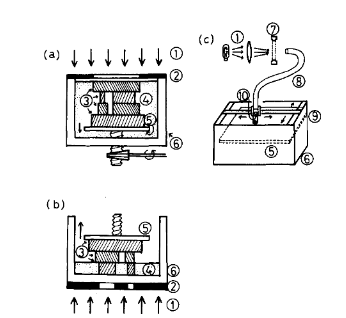
\includegraphics[scale=0.5]{figuras/metodos_Kodama1981.png}
    \caption{Métodos descritos por Kodama \cite{Kodama1981}.}
    \label{fig:metodos_Kodama1981}
\end{figure}

Poco tiempo después -en 1984- el norteamericano Charles Hull desarrollaría la técnica de \acrfull{SLA}. La \acrlong{SLA} utilizaba polímeros sensibles a la luz que se depositaban por capas sobre una cama móvil. Los primeros trabajos de Hull se trataban de versiones miniaturizadas de objetos diseñados con \acrshort{CAD}. Dichos diseños podían fabricarse rápidamente y se utilizaban en labores de prototipado. El éxito fue tan grande que dio origen a su propia familia de procesos \acrshort{AM} (los \acrshort{VPP}) y además permitió a Hull fundar la primera compañía de fabricación aditiva de la historia: 3DSystems \cite{web_3DSystems}. En la figura \ref{fig:patente_sla} se muestra el primer modelo de estereolitografía. \label{sec:esterilitografia}

\begin{figure}[h!]
    \centering
    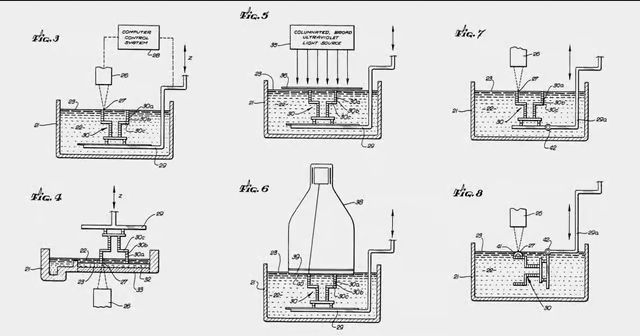
\includegraphics[scale=0.30]{figuras/patente_sla.png}
    \caption{Primer modelo de \acrshort{SLA} patentado \cite{Hull1984}.}
    \label{fig:patente_sla}
\end{figure}

El proceso de fabricación aditiva más conocido es el de \acrfull{MEX}, cuyo primer desarrollo corrió a cargo del ingeniero Scott Scrump en 1989 \cite{Scrump1989}. En el año 2005, las patentes de Scrump (Figura \ref{fig:patente_scrump}) fueron liberadas y el desarrollo de nuevas máquinas \acrshort{AM} tuvo un auge nunca antes visto gracias a la proliferación de movimientos basados en el código abierto como RedRap (Figura \ref{fig:maquina_redrap1}) \cite{web_RedRap}. Iniciativas de este tipo han permitido que la fabricación aditiva haya podido llegar a multitud de empresas y hogares, favoreciendo la inversión y la aparición de nuevas tecnologías derivadas.

\begin{figure}[h!]
    \centering
    \begin{subfigure}[h]{0.45\linewidth} 
        \centering
        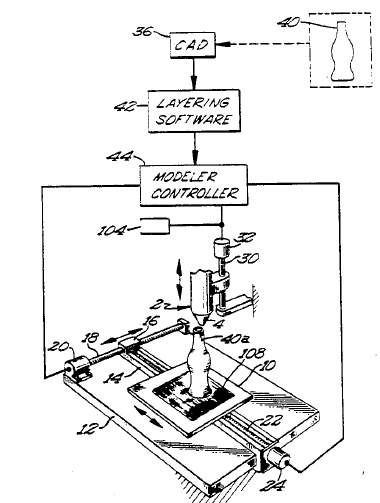
\includegraphics[scale=0.38]{figuras/patente_scrump.png}
        \caption{Sistema \acrshort{MEX} \cite{Scrump1989}.}
        \label{fig:patente_scrump}
    \end{subfigure}
    \begin{subfigure}[h]{0.45\linewidth} 
        \centering
        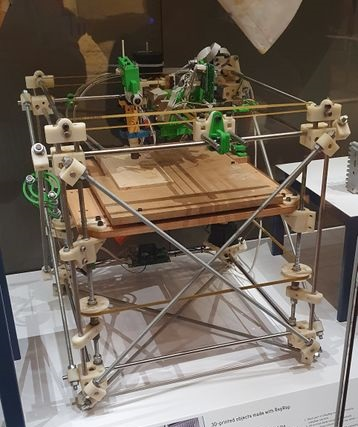
\includegraphics[scale=0.3]{figuras/maquina_redrap1.jpg}
        \caption{Primera máquina RedRap \cite{web_RedRap}.}
        \label{fig:maquina_redrap1}
    \end{subfigure}
    \caption{Comienzos de la \acrshort{MEX}}
    \label{fig:FDM_y_redrap}
\end{figure}

\subsection{Aplicaciones de la fabricación aditiva}
En los últimos años la \acrshort{AM} ha permitido el desarrollo de piezas altemente personalizadas con una variedad de materiales como madera, aleaciones metálicas, cerámicas o polímeros de diferentes propiedades. Esto es, se ha pasado de ser un campo centrado fundamentalmente en el prototipado de piezas, al diseño de elementos complejos de gran precisión y adaptabilidad. Algunos ejemplos de los sectores de aplicación más representativos son:

\begin{itemize}
    \item \textbf{Transporte aeroespacial}\\
    La AM es especialmente útil en aplicaciones que suponen un compromiso entre el volumen de producción y las exigencias técnicas. En este caso, los materiales más empleados son diferentes aleaciones metálicas. Estas aleaciones se utilizan para soportar las condiciones de críticas de presión y temperatura de ciertos componentes como motores a reacción o fuselaje de aviones \cite{BlakeyMiner2021}. En la figura \ref{fig:am_aplicaciones_aerol} se observa un prototipo a escala de un motor a reacción realizado mediante estas técnicas.
    
    \item \textbf{Automoción}\\
    La industria del automóvil sigue una línea similar a la aeroespacial. En este caso, las aplicaciones más notables se encuentran focalizadas en la optimización de material. Con ayuda de estos sistemas, se obtiene un prototipo impreso y, si los ensayos son exitosos, existe la posibilidad de disponer el modelo final en una matriz de impresión \cite{Zhao_2023}. La figura \ref{fig:am_aplicaciones_automovil} ilustra un ejemplo, a la izquierda se presenta el diseño original y la derecha el resultante de la optimización topológica, ambos hechos con \acrshort{AM}.
    
    \begin{figure}[h!]
        \centering
        \begin{subfigure}[h]{0.45\linewidth} 
            \centering
            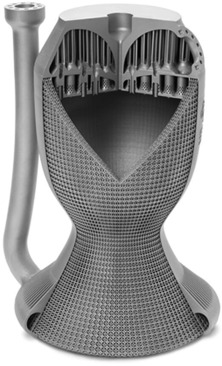
\includegraphics[scale=0.4]{figuras/am_aplicaciones_aero.jpg}
            \caption{Prototipo de motor a reacción \cite{BlakeyMiner2021}}
            \label{fig:am_aplicaciones_aerol}
        \end{subfigure}
        \begin{subfigure}[h]{0.4\linewidth} 
            \centering
            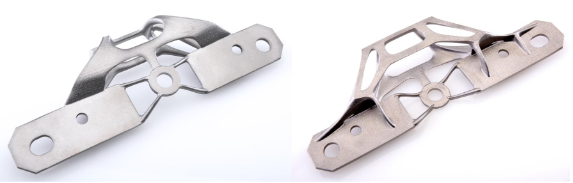
\includegraphics[scale=0.45]{figuras/am_aplicaciones_automovil.png}
            \caption{Bastidor hecho con \acrshort{AM} \cite{Zhao_2023}.}
            \label{fig:am_aplicaciones_automovil}
        \end{subfigure}
        \caption{Sector aeroespacial y automovilístico}
        \label{fig:FDM_y_redrap}
    \end{figure}

    \item \textbf{Sistemas electrónicos}\\
    Una de las ventajas más destacadas de la fabricación aditiva en el ámbito de los componentes electrónicos es su capacidad para delinear con precisión las diferentes regiones portadoras de electrones en componentes activos como diodos, transistores, amplificadores operacionales, y transistores bipolares de puerta aislada (IGBT) entre otros \cite{Bellacicca2018}\cite{Zhang2015}. Esta precisión a escala de micras es fundamental para garantizar el rendimiento óptimo de los dispositivos electrónicos, ya que permite un control más preciso del flujo de corriente eléctrica y facilita la integración de componentes en sistemas más complejos.
    
    Gracias a esta ventaja, la fabricación aditiva ha resultado de gran importancia para el descenso de los costes de la electrónica industrial y de consumo. La figura \ref{fig:am_aplicaciones_electronica} muestra un sensor luminoso con un amplificador operacional fabricado mediante esta técnica.

    \item \textbf{Diseño de materiales}\\
    La investigación en nuevos materiales va dirigida en los últimos años hacia métodos de fabricación que incluyan aleaciones con composición variable según el gradiente de tensiones. Los resultados más notables se han alcanzado con aleaciones que disponen de Ni y  Ti como principales constituyentes \cite{Li2019}. Otro campo interesante es la conocida como \textit{impresión 4D} \cite{Mahmood2023}, esto es, la impresión 3D de materiales cuyas propiedades cambian ante estímulos térmicos, eléctricos o luminosos. La figura \ref{fig:am_aplicaciones_materiales} muestra el cambio de forma de varios componentes hechos con AM ante elevadas temperaturas.

    \begin{figure}[h!]
        \centering
        \begin{subfigure}[h]{0.45\linewidth} 
            \centering
            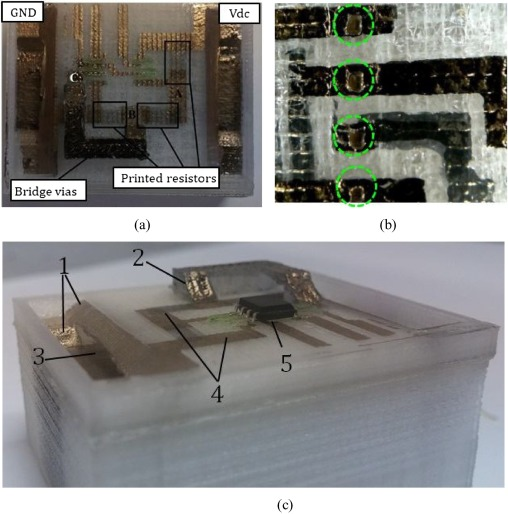
\includegraphics[scale=0.3]{figuras/am_aplicaciones_electronica.jpg}
            \caption{Sensor luminoso impreso en 3D \cite{Bellacicca2018}.}
            \label{fig:am_aplicaciones_electronica}
        \end{subfigure}
        \begin{subfigure}[h]{0.45\linewidth} 
            \centering
            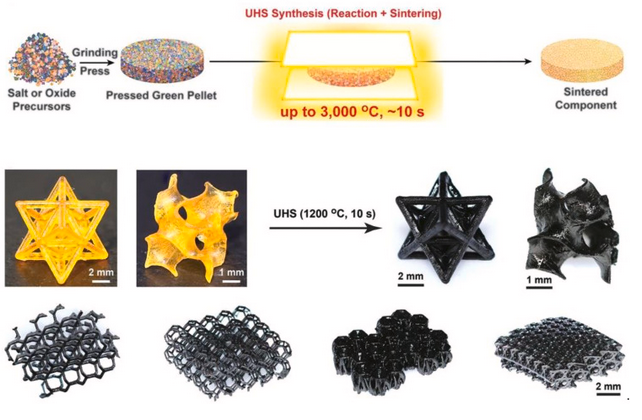
\includegraphics[scale=0.25]{figuras/am_aplicaciones_materiales.png}
            \caption{Demostración de composite hecho con impresión 4D \cite{Mahmood2023}.}
            \label{fig:am_aplicaciones_materiales}
        \end{subfigure}
        \caption{Fabricación electrónica y nuevos materiales}
        \label{fig:FDM_y_redrap}
    \end{figure}
    
    \item \textbf{Sector médico}\\
    La fabricación aditiva está ganado un rol de especial importancia en las especialidades médico-quirúrgicas. Algunas de las especialidades más demandadas son neurocirugía \cite{Guarino2021}, cirugía oral y maxilofacial \cite{Zoabi2022} o cirugía cardiaca \cite{Vukicevic2017}. Como norma general, los materiales más utilizados en estas aplicaciones son polímeros como \acrshort{ABS} y \acrshort{PLA} o resinas mezcladas con polvos cerámicos \cite{Kumar2021}. Cualquier aplicación de la \acrshort{AM} en este campo debe tener en cuenta siempre un condicionante: la no interferencia con pruebas diagnósticas en las que se irradie algún tipo de energía como pueden ser rayos X o imágenes de resonancia magnética. 
    
    La figura \ref{fig:am_aplicaciones_medico} muestra una reconstrucción de mandíbula hecha con un proceso \acrshort{AM}. Se ha empleado una imagen diagnóstica para elaborar una fédula personalizada para un caso clínico con el mentón completamente fracturado. A través de distintas iteraciones se pudo desarrollar un implante que resultase cómodo para el paciente y redujese el tiempo de operación.

    \begin{figure}[h!]
        \centering
        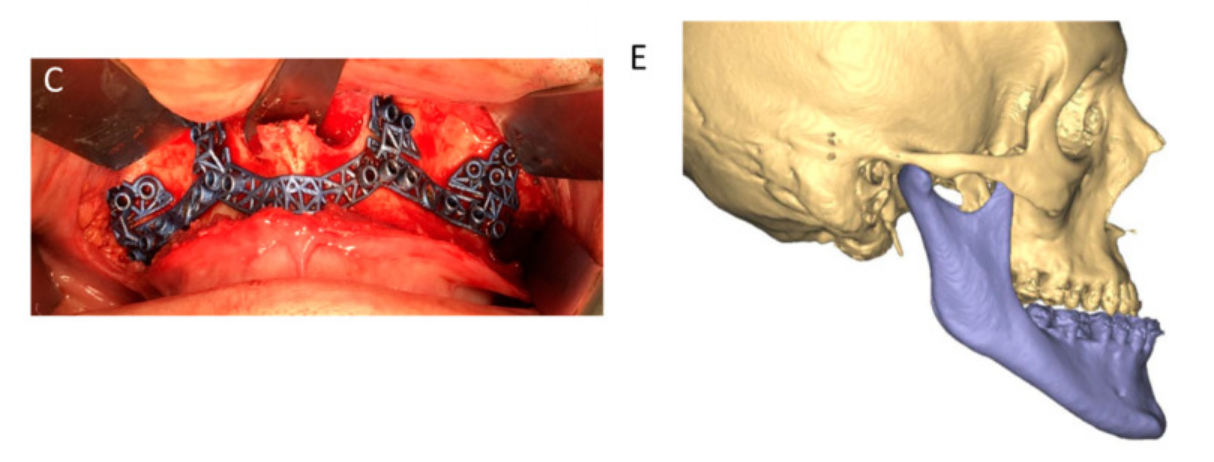
\includegraphics[scale=0.25]{figuras/am_aplicaciones_medico.png}
        \caption{Fédula mentoniana para reconstrucción de mandíbula \cite{Zoabi2022}.}
        \label{fig:am_aplicaciones_medico}
    \end{figure}
\end{itemize}

\section{Estado del arte}
Esta sección sirve para establecer un resumen de los últimos avances realizados en el campo de la fabricación aditiva robotizada, haciendo un especial hincapié en los modelos de geometrías no planares. Para ofrecer una perspectiva sencilla de comprender y centrar el enfoque en el desarrollo de una arquitectura de estación de este tipo, se establecen tres puntos principales.

El primer punto describirá el funcionamiento básico de un sistema de fabricación aditiva y describirá el flujo de trabajo que acompaña a este tipo de procesos. El segundo introducirá al lector en las tecnologías \acrshort{AM} robotizables mencionando aquellas con más facilidad para integrar este tipo de equipos, indicando las operaciones de mayor importancia y presentando algunas de las arquitecturas informáticas de estación robotizadas que han servido de referencia para este trabajo. El tercer y último punto se enfocará en la presentación de las tecnologías \acrshort{NPAM}. En él se comentarán sus principales ventajas y limitaciones, así como también pueden verse favorecidas por la integración de equipos robóticos en su flujo de trabajo.

\subsection{Fabricación aditiva convencional}
\subsubsection*{Funcionamiento básico}
\hypertarget{Funcionamiento básico}{}
\bookmark[level=subsubsection,dest=Funcionamiento básico]{Funcionamiento básico}

Como se ha indicado en líneas anteriores, la fabricación aditiva convencional utiliza un extrusor de material que termina depositándose sobre una cama plana.  El extrusor puede desplazarse en las configuraciones cinemáticas del espacio cartesiano (ejes XYZ) mientras la cama de impresión\footnote{Superficie sobre la que se va depositando el material} permanece quieta, o puede combinar su movimiento con el de un soporte móvil.

En las tecnologías \acrshort{MEX} convencionales, el material se encuentra inicialmente en forma de filamento flexible y para depositarse sobre la cama de impresión debe estar en un estado viscoso y fácilmente maleable. El mecanismo que aporta el calor y la presión necesarios para que tome esa consistencia es el extrusor. El extrusor se encuentra conectado a una pequeña unidad de cómputo que posee capacidad para determinar parámetros como: posición del extrusor, temperatura del material y velocidad de deposición del filamento.

Comúnmente se considera a las impresoras 3D comerciales como los ejemplos típicos de las tecnologías \acrshort{AM} tradicionales. El auge de este tipo de equipos ha permitido que cada fabricante desarrolle su propia variante de la estrategia propuesta. En la figura \ref{fig:impresora3d_1} se observa una estación de impresión 3D comercial, en la que el fabricante ha optado por un extrusor móvil en la dirección vertical y una horizontal, con una cama con movilidad en la dirección horizontal restante. La figura \ref{fig:impresora3d_2} muestra otra estación comercial, en este caso la cama permanece inmóvil y el extrusor es el único elemento móvil.

\begin{figure}[h!]
     \begin{subfigure}[h]{0.45\linewidth} 
        \centering
        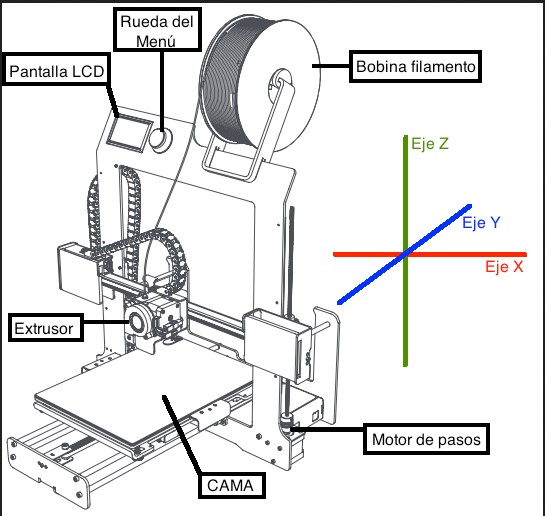
\includegraphics[scale=0.4]{figuras/impresora3d_1.jpg}
        \caption{Impresora 3D con extrusor y cama móvil \cite{GobCanarias}.}
        \label{fig:impresora3d_1}
    \end{subfigure}
    \begin{subfigure}[h]{0.45\linewidth} 
        \centering
        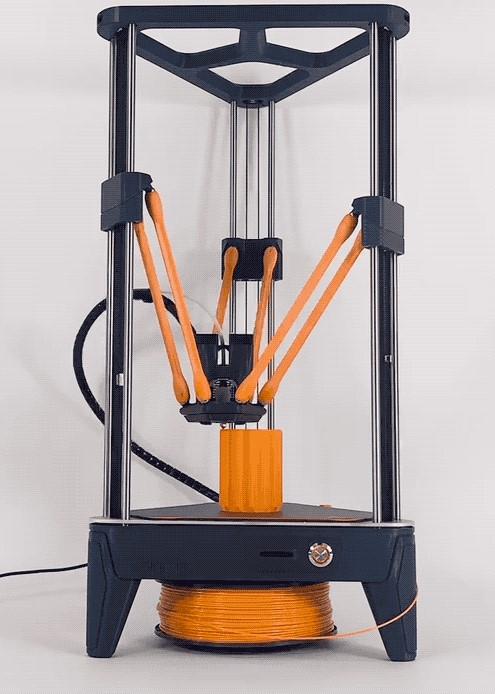
\includegraphics[scale=0.3]{figuras/impresora3d_2.jpg}
        \caption{Impresora 3D con únicamente extrusor móvil \cite{impresoraDagoma}.}
        \label{fig:impresora3d_2}
    \end{subfigure}
    \caption{Esquemas de movimiento en \acrshort{AM} tradicional.}
\end{figure}

\subsubsection*{Flujo de trabajo}
\hypertarget{Flujo de trabajo}{}
\bookmark[level=subsubsection,dest=Flujo de trabajo]{Flujo de trabajo} \label{sec:flujo_trabajo}

 Los métodos de \acrshort{AM} convencionales comienzan con la generación de un fichero \acrshort{CAD} en 3D. Las superficies que definen el modelo se dividen en pequeños fragmentos triangulares en un proceso conocido como \textit{teselado}. El resultado del teselado queda representado en un archivo \acrshort{STL}, un formato estandarizado que consiste en una lista de superficies triangulares distribuidas por el espacio. Estas superficies están definidas por los vértices de cada triángulo y el vector normal al plano que conforman \cite{Brown2014}\cite{Thompson2016}. 

El fichero \acrshort{STL} representa un concepto sencillo de comprender y apto para multitud de algoritmos, no obstante su uso implica tres inconvenientes fundamentales:
\begin{itemize}
    \item \textbf{Tamaño creciente:} A mayor grado de teselado, se necesita una mayor cantidad de triángulos que representar en el fichero. En otras palabras, se requiere de una capacidad de cómputo cada vez más grande \cite{Gibson2017}.
    \item \textbf{Problemas de exactitud:} Muchos diseños \acrshort{CAD} poseen curvas difíciles de parametrizar para los algoritmos de teselado. Motivo por el que en muchas ocasiones se realiza una aproximación con triángulos y se introduce un factor de error numérico a compensar \cite{Gohari2016}.
    \item \textbf{Propiedades del material:} El proceso de teselado en ningún instante toma en cuenta el material del que estará hecha la pieza final. A causa de esta falta de información, es común que en ocasiones se deban combinar varios archivos \acrshort{STL} para elaborar una única pieza \cite{Yang2017}.
\end{itemize}

Al final la calidad del \acrshort{STL} dependerá de dos variables esenciales, ambas a minimizar para alcanzar la máxima precisión \cite{Pinar2019}:
\begin{itemize}
    \item \textbf{Tolerancia cordal:} Es la máxima distancia admitida entre el punto real definido por la superficie del modelo CAD y el punto aproximado por el proceso de teselado.
    \item  \textbf{Ángulo de control:} Dada una sección de la curva trazada por el CAD, es el giro existente entre la propia curva del modelo original y la recta trazada por el proceso de teselado.
\end{itemize}

Después del teselado, la figura pasa a ser recortada en multitud de secciones representadas por un archivo \acrshort{STL} en un proceso conocido como \textit{slicing}. Este archivo servirá como base para obtener las instrucciones en formato \acrshort{AMF}\footnote{Fichero que define el modelo de datos que debe seguir la representación de la pieza objetivo del proceso aditivo. Contiene una parametrización de las superficies 3D que describen la geometría del objeto incluyendo soporte para otros metadatos (color, chaflanes, soportes, etc). La máquina calcula automáticamente el movimiento de sus actuadores a partir de esta información} para la impresión final. El \textit{slicing} puede ser uniforme o adaptativo \cite{Pinar2019}. En el primero, todos los planos del fichero \acrshort{STL} se consideran de grosor constante y el coste computacional es menor. En el segundo, los planos del fichero \acrshort{STL} tienen una anchura variable, lo que ayuda a optimizar material y tiempo a coste de una mayor demanda computacional. 

Con el \acrshort{AMF} ya obtenido, en procesos \acrshort{AM} típicos sólo queda cargarlo en la memoria de la máquina. Con esta información cargada, el microcontrolador integrado en la máquina calculará las velocidades e inercias necesarias para desplazar el extrusor a las posiciones indicadas. Este enfoque se aprecia en la figura \ref{fig:flujo_trabajo_normal}. 

\begin{figure}[h!]
    \centering
    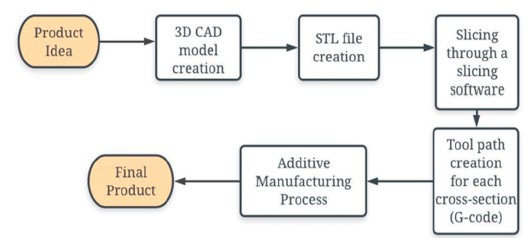
\includegraphics[scale=0.5]{figuras/flujo_trabajo_normal.jpg}
    \caption{Flujo de trabajo convencional \cite{Pinar2019}}
    \label{fig:flujo_trabajo_normal}
\end{figure}

Una parte de la investigación actual del campo de la fabricación aditiva está centrada en la búsqueda de nuevos algoritmos de teselado y \textit{slicing}. Uno de sus objetivos más conocidos la minimización de soportes en voladizo requeridos por figuras complejas \cite{Coupek_2018}, pero también existen otros trabajos enfocados en otros aspectos como la reducción de tiempos de impresión \cite{Karkaria_2024}, el aumento  de propiedades mecánicas \cite{Rosso_2021} o la mejora de acabados finales.

\subsection{Fabricación aditiva robotizada}
El \textit{slicing} uniforme y el adaptativo fueron planteados para sistemas \acrshort{AM} que trabajasen con láminas planas y siempre en la misma dirección. Con el paso del tiempo, se ha podido imprimir cuerpos geométricamente más complejos con la introducción de más grados de libertad. Es decir, se han podido definir una variedad más grande de direcciones de apilamiento de capas y ya no es estrictamente necesario emplear geometrías planas de deposición de material. Esto implica sistemas más precisos y complejos, capaces de asistir en labores de impresión con múltiples direcciones. Es decir, se pasa a emplear manipuladores con configuraciones cinemáticas demás de 3 \acrshort{DOF}, como pueden ser brazos robóticos industriales o de tipo colaborativo entre otros.



\subsubsection*{Tecnologías AM robotizables}
\hypertarget{Tecnologías AM robotizables}{}
\bookmark[level=subsubsection,dest=Tecnologías AM robotizables]{Tecnologías AM robotizables}
Dentro de las diferentes familias de procesos descritas por la norma ISO de fabricación aditiva \cite{ISO-ASTM-52900-2022}, aquellos que pueden integrar fácilmente un manipulador robótico en su flujo de trabajo son los procesos \acrshort{MEX} y \acrshort{DED}. Pese a que existen avances en tecnologías que dispensan gotas de un fotopolímero líquido -como el trabajo de Li et al. \cite{Li_2017}, inspirado en las tecnologías \acrshort{VPP}-  con ayuda de un manipulador robótico, sus aplicaciones por el momento son escasas y se encuentran limitadas a un nicho dentro de aplicaciones biomédicas con hidrogeles específicos. En las siguientes líneas se describirán las dos tecnologías mayoritarias comentando algunas de las aplicaciones más usuales.

\begin{itemize}
    \item \textbf{\acrfull{MEX}}\\
    Es el método más empleado en la fabricación aditiva tradicional. Consiste en una cabeza móvil que toma un filamento de termoplástico y lo funde aportando calor y presión mediante un proceso de extrusión. Algunos de los materiales más empleados son polímeros como el \acrshort{ABS} o el \acrshort{PLA}. No obstante, el ser el método \acrshort{AM} más extendido ha permitido que con el paso del tiempo hayan surgido desarrollos que empleen otros materiales como cera, metales o mezclas de polvos cerámicos \cite{Kruth1998}. También se ha innovado en las técnicas de extrusión de material, de modo que existen equipos que combinan varios extrusores favoreciendo la reducción de costes o el uso conjunto de varios materiales.

    Las piezas resultantes de este proceso se caracterizan por tener un tamaño compacto y por requerir un coste reducido en tareas de acabado y mantenimiento. La figura \ref{fig:zhang_2016_ejemplo_mex_robot} muestra una máquina \acrshort{MEX} robotizada realizada por Zhang et al. \cite{Zhang_2016} En este caso se utilizó un robot ABB  con un extrusor de fabricación propia acoplado (imagen \textit{(a)}) . Para visulizar una imagen previa de la pieza y simular los movimientos del manipulador se utilizó el software de cálculo nativo de ABB (imagen \textit{(b)}. Este ejemplo ha utilizado como material de referencia el \acrshort{ABS} (imagen \textit{(c)}), pero puede extenderse a otros filamentos poliméricos como \acrshort{PLA} o fibras continuas de carbono o vidrio para la producción de composites.

    \begin{figure}[h!]
        \centering
        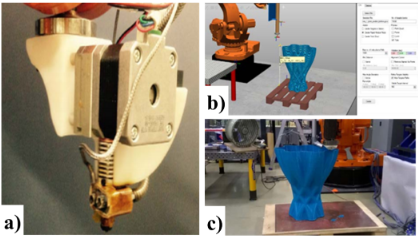
\includegraphics[scale=0.4]{figuras/zhang_2016_ejemplo_mex_robot.png}
        \caption{Estación \acrshort{MEX} robotizada \cite{Zhang_2016}}
        \label{fig:zhang_2016_ejemplo_mex_robot}
    \end{figure}

    \item \textbf{\acrfull{DED}}\\
    Este método emplea una fuente de calor para fundir el material de fabricación mientras se va depositando sobre la superficie de impresión. En concreto, el término hace referencia a que la fuente de energía (láser, haz de electrones o arco de plasma entre otros) tiene el objetivo de derretir un filamento sólido de material para que caiga de forma controlada sobre la cama de impresión. Este proceso se caracteriza por ser el único con capacidad para procesar componentes metálicos, bien sea en forma de polvo o de filamento. Algunas de las aplicaciones de este proceso son la elaboración de geometrías complejas con aleaciones de alta densidad \cite{Caiazzo_2018} o la creación de recubrimientos multimaterial con resistencia a altas temperaturas y la abrasión química \cite{Fujishima_2017}. 

    Estos sistemas presentan ciertas limitaciones en cuanto al elevado número de parámetros de control (potencia del láser, velocidad de alimentación de material, distancia de trabajo, propiedades del material, ángulo de deposición del material, etc.) o la construcción de formas complejas. A causa de estas limitaciones, existe un amplio campo de investigación para optimizar esta tecnología. El trabajo de Ding et al. \cite{Ding_2016} está enfocado en integrar un sistema de deposición láser móvil con una plataforma móvil para reorientar paulatinamente la pieza resultado según se fabrica (Figura \ref{fig:ejemplo_ding_2016}). Por su parte, empresas como Meltio \cite{Meltio_web} son especialistas en deposición por arco de plasma y su integración con sistemas robotizados ya existentes, como puede verse en la Figura \ref{fig:ejemplo_meltio}.

    \begin{figure}[h!]
        \centering
         \begin{subfigure}[h]{0.45\linewidth} 
            \centering
            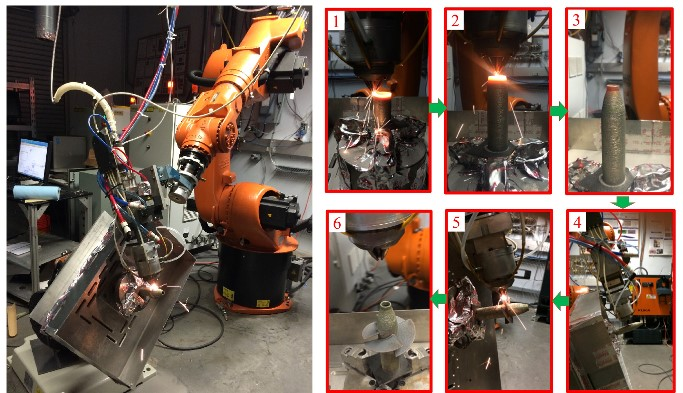
\includegraphics[scale=0.35]{figuras/ejemplo_ding_2016.jpg}
            \caption{Deposición láser móvil robotizada \cite{Ding_2016}}
            \label{fig:ejemplo_ding_2016}
        \end{subfigure}
        \begin{subfigure}[h]{0.45\linewidth} 
            \centering
            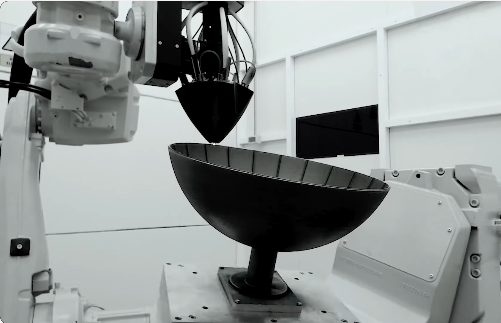
\includegraphics[scale=0.45]{figuras/ejemplo_meltio.png}
            \caption{Arco de plasma robotizado \cite{Meltio_web}.}
            \label{fig:ejemplo_meltio}
        \end{subfigure}
        \caption{Procesos \acrshort{DED}}
    \end{figure}

    
\end{itemize}
 
Cuando se pretende emplear un brazo robótico en el proceso de fabricación aditiva, la literatura tiende a referirse a él como un proceso de \textit{Impresión con manipuladores de más de 3 \acrshort{DOF}}. El brazo robótico puede modificar con gran precisión la trayectoria y velocidad de deposición del material. El manipulador puede operar directamente el extrusor o la cama de impresión, lo cual le dota de una gran libertad de movimiento para conseguir diseños no planares. Este es el modelo de impresión \acrshort{NPAM} utilizado en este trabajo. La figura \ref{fig:impresion_3d_robotica} es un ejemplo de una estación con 8 \acrshort{DOF}, donde 6 corresponden al robot y 2 a la cama de impresión móvil.

\begin{figure}[h!]
    \centering
    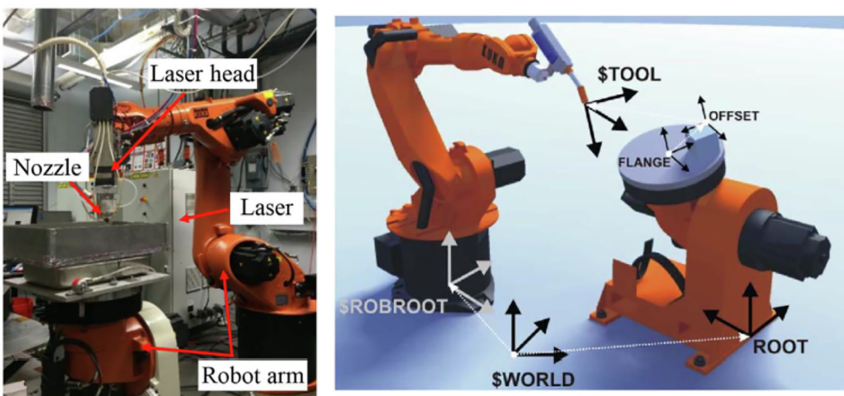
\includegraphics[scale=0.3]{figuras/impresion_3d_robotica.png}
    \caption{Impresión robótica con 8 \acrshort{DOF} \cite{Shah_2022}}
    \label{fig:impresion_3d_robotica}
\end{figure}

\subsubsection*{Preparación del manipulador}
\hypertarget{Preparación del manipulador}{}
\bookmark[level=subsubsection,dest=Preparación del manipulador]{Preparación del manipulador}

La literatura establece que los procesos de fabricación pueden transcurrir cíclicamente a lo largo de un intervalo de tiempo conocido como tiempo de ciclo \cite{Kalpajkin_2006}. El tiempo de ciclo puede establecerse como la sucesión de cuatro etapas directamente relacionadas con la manipulación de materia prima y la elaboración del producto industrial: espera, preparación, operación y post-procesado.

La figura \ref{fig:tiempo_ciclo} muestra un esquema de cómo se suceden estas etapas durante el tiempo de ciclo del proceso. Nótese que en los extremos de esta sucesión también se define una cantidad de tiempo variable correspondiente al transporte de información, materiales, equipos y mano de obra entre procesos.

\begin{figure}[h!]
    \centering
    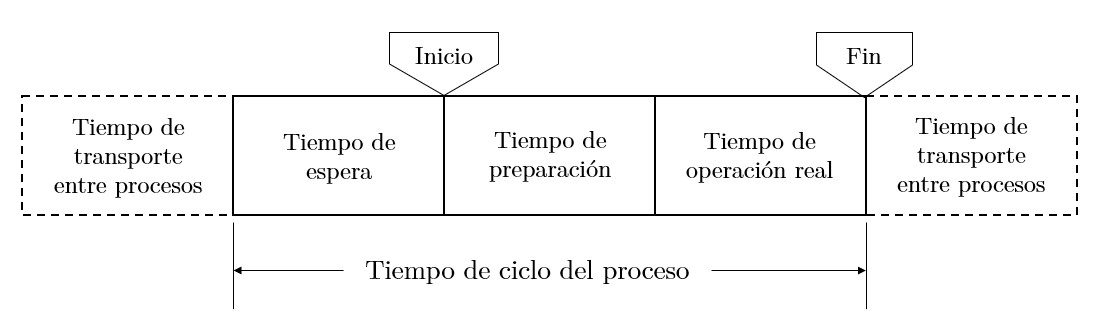
\includegraphics[scale=0.4]{figuras/tiempo_ciclo_v2.jpg}
    \caption{Etapas del tiempo de ciclo \cite{Kalpajkin_2006}}
    \label{fig:tiempo_ciclo}
\end{figure}

Un proceso de fabricación aditiva robotizada también sigue esta estructura. La etapa de preparación, en concreto, es de vital importancia para calibrar con antelación todos los sistemas que participarán en el proceso. Independientemente del elemento móvil que se desee integrar con el robot, siempre es necesario implementar una serie de sistemas que permitan calcular una trayectoria que debe seguir el manipulador y que puedan compensar las inercias y desplazamientos no deseados del robot. Para ello se establece un procedimiento durante la etapa de preparación denominado \textit{calibración} en el que se define la posición del manipulador en el espacio de trabajo y se estudia el trazado de trayectorias simples, así como también en otros sistemas de referencia asociados a un sistema global.

Durante la calibración es posible extraer los factores que pueden intervenir en el desvío existente entre la trayectoria que se proyecta en el diseño \acrshort{CAD} de la pieza, la calculada por el software del manipulador y la efectuada por manipulador en sí. La calibración puede ser de dos tipos diferentes:

\begin{itemize}
    \item \textbf{Calibración extrínseca:} Centrada en determinar las relaciones existentes entre los sistemas de coordenadas empleados por el robot y su entorno exterior que lo rodea. Algunos de los métodos de calibración extrínseca que han tenido mejores resultados son los propuestos por Kato et al. \cite{Kato_2021}, que se basa en el uso de un algoritmo de árbol de decisión para corregir la desviación existente entre la pose cartesiana calculada y la alcanzada en la realidad; Zheng et al. \cite{Zheng_2022}, que implementa algoritmos genéticos para corregir las funciones objetivo que minimicen la desviación de las posiciones tras varias iteraciones consecutivas; o por Guzmán et al.\cite{Guzman_2023} que propone un flujo de trabajo generalizado adaptable a varias estaciones y fundamentado en obtener la calibración de zonas clave de la estación de trabajo e ir relacionándolas de forma sucesiva con unos utillajes diseñados especialmente para dicha función.

    \item \textbf{Calibración intrínseca:} Enfocada en determinar aquellos parámetros geométricos, dinámicos, eléctricos y de control del propio robot que pueden influir en su comportamiento. Métodos de este tipo de calibración notables son los aportados por Nubiola et al.\cite{Nubiola2013}, que analiza las inercias asociadas a cada eslabón y articulación de un robot manipulador y propone una serie de funciones que minimizan los errores de cálculo de coordenadas articulares en la fase de cálculo de trayectoria software del robot; el trabajo de Moller et al.\cite{Moller_2017} enfocado en establecer un bucle de control con los encoders de cada articulación para reducir su inercia de giro y poder corregir las diferentes posiciones calculadas de forma previa a la ejecución; o el definido por Villagrossi et al.\cite{Villagrossi2018} que entrelaza tres bucles de control enfocados en modificar en tiempo real la alimentación de material, el ángulo de ataque adoptado por la herramienta y la fuerza final ejercida por el manipulador.
\end{itemize}

\subsubsection*{Sistemas de referencia y métodos de aprendizaje}
\hypertarget{Sistemas de referencia y métodos de aprendizaje}{}
\bookmark[level=subsubsection,dest=Sistemas de referencia y métodos de aprendizaje]{Sistemas de referencia y métodos de aprendizaje}

En cualquier proceso de fabricación robótica siempre será necesario disponer de al menos tres sistemas de referencia (Figura \ref{fig:Robotics-coordinate-systems}). Estos sistemas deben relacionarse entre sí para definir el proceso de fabricación. Estos son: (1) sistema de referencia de la máquina, (2) sistema de referencia de la pieza y (3) sistema de referencia de la herramienta.

Dependiendo de la aplicación, se pueden añadir más sistemas de referencia y enlazarlos mutuamente. No obstante, se debe tener en cuenta que los sistemas de referencia disponibles deben relacionarse a través de una serie de transformaciones matriciales que permitan definir de forma unívoca el movimiento del robot.
    
\begin{figure}[h!]
    \centering
    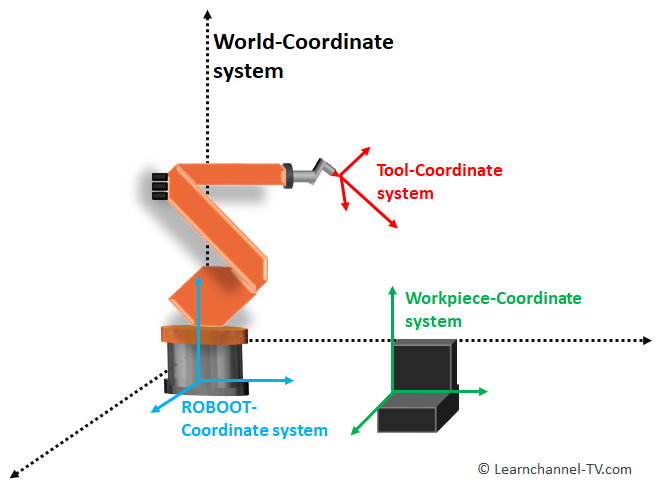
\includegraphics[scale=0.4]{figuras/Robotics-coordinate-systems.png}
    \caption{Sistemas de coordenadas de un robot \cite{Robot_Coordinate_Systems}}
    \label{fig:Robotics-coordinate-systems}
\end{figure}

La trayectoria puede obtenerse a gracias a los \textit{métodos de aprendizaje}, un conjunto de operaciones que permite al robot y su controlador calcular los puntos de la trayectoria y definir los pares y velocidades necesarios para llevarla a cabo. Los métodos de aprendizaje pueden clasificarse como:
\begin{itemize}
    \item \textbf{Aprendizaje \textit{online} o in-situ:} Se despalaza el robot manualmente a los puntos deseados de la trayectoria para registrarlos uno a uno e implementar un controlador especialmente definido para ese movimiento. Pese a que este tipo de aprendizaje aporta una precisión del orden de la repetibilidad\footnote{Capacidad de un mecanismo automático para retornar a la posición inicial varias veces siempre bajo las mismas condiciones} de la unidad empleada, sus mayores inconvenientes son que requiere de un tiempo elevado de preparación y debe repetirse la operación cada vez que se haga una nueva configuración a la estación. 
    \item \textbf{Aprendizaje \textit{offline} o planificado:} La trayectoria se plantea de forma teórica gracias a diferentes aplicaciones software y se traslada a un código ejecutable por el robot físico \cite{Botazzi_2005}. Estos métodos de aprendizaje necesitan usualmente de un marco de referencia que represente su entorno real. Las soluciones más empleados habitualmente son integrar un modelo \acrshort{CAD} en el espacio de trabajo virtual \cite{Botazzi_2006} o reconstruir el objeto real a partir de sistemas de visión por computador \cite{Liu_2010}.
    \item \textbf{Aprendizaje híbrido:} Este método emplea un flujo de trabajo basado en una combinación de los dos anteriores. En una primera fase se define una trayectoria concreta y se indica al robot cómo alcanzar el primer punto mediante un proceso de aprendizaje online. Cuando el robot ha podido desplazarse desde su pose original a la pose comienzo de la trayectoria objetivo, se inicia inmediatamente una segunda fase de aprendizaje offline en la que se calcula el trazado del resto de puntos de la trayectoria. Uno de los usos con más potencial de estos sistemas de aprendizaje es la corrección dinámica -mientras se efectúa el proceso de fabricación- de desviaciones existentes entre la pieza real y el modelo \acrshort{CAD} \cite{Zheng_2022}.
\end{itemize}
    
Una representación simple de los métodos de aprendizaje online y offline puede verse en la Figura \ref{fig:aprendizaje_online_offline}. En los años recientes, el aprendizaje offline está cobrando una relevancia especial de cara a los procesos robotizados gracias a la mayor versatilidad que aporta en el cálculo y trazado de trayectorias, que pasa a ser responsabilidad de una capa de software especializado. Las técnicas de aprendizaje offline en muchas ocasiones necesitan acompañarse de técnicas de calibración extrínseca de alta fiabilidad para garantizar la ejecución de la trayectoria calculada y también la integridad del equipo empleado junto a sus usuarios.

\begin{figure}[h!]
    \centering
    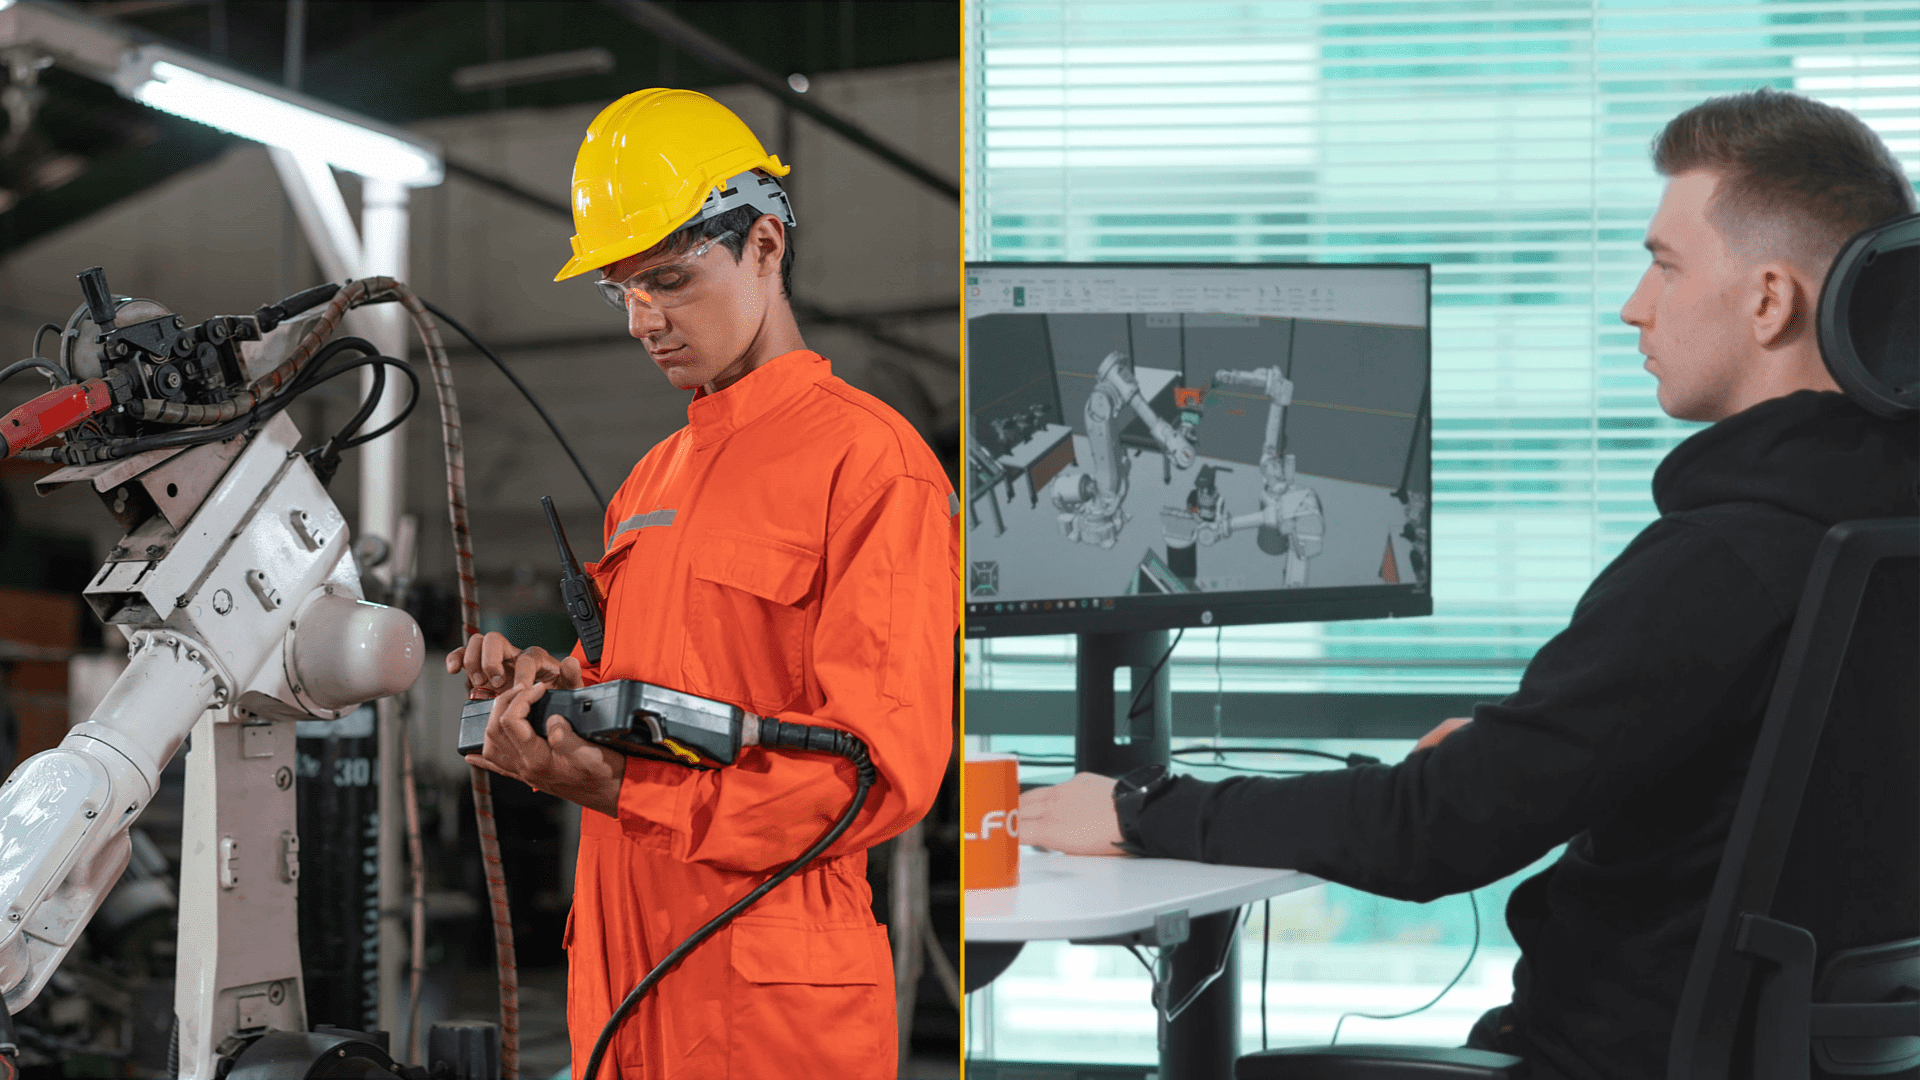
\includegraphics[scale=0.15]{figuras/aprendizaje_online_offline.png}
    \caption{Ejemplo de aprendizaje online (izquierda) y offline (derecha)}
    \label{fig:aprendizaje_online_offline}
\end{figure}

\subsubsection*{Arquitecturas informáticas}
\hypertarget{Arquitecturas informáticas}{}
\bookmark[level=subsubsection,dest=Arquitecturas informáticas]{Arquitecturas informáticas}
\label{sec: arquitecturas_informaticas_estado_arte}

Las tareas antes vistas suponen operaciones matemáticamente complejas que deben realizarse con ayuda de un equipo software especializado. Por otro lado, el brazo robótico debe poder comunicarse con otros elementos de su espacio de trabajo para disponer de información constante acerca de parámetros cinemáticos (posición, velocidad y aceleración), dinámicos (fuerzas y torques articulares), materiales (temperatura, presión y flujo) o mandatos del operario humano. 

El manipulador robótico por sí solo no es suficiente para gestionar todo este volumen de información y necesita de elementos auxiliares. Es decir, el brazo robótico debe formar parte de una arquitectura de comunicaciones industriales más grande.

Para poder integrar el manipulador robótico en este tipo de arquitecturas, se deben introducir modificaciones al flujo de trabajo explicado en la sección \ref{sec:flujo_trabajo}. La figura \ref{fig:flujo_trabajo_robot} sirve de ejemplo, en este caso se toma el trabajo de un equipo del Virginia Tech con un robot ABB  1200-7 \cite{Kubalak2016}. Su mayor aporte es la introducción de una unidad de control responsable del proceso de \textit{parseo} \footnote{Conjunto de operaciones de lectura de un fichero estandarizado para obtener los parámetros más representativos en un proceso automatizado. En la literatura de la \acrshort{AM} se puede interpretar como la lectura del código \acrshort{AMF} para trazar la trayectoria de los elementos móviles.} a partir del \acrshort{AMF} que además establezca una realimentación interna con las articulaciones del robot para corregir trayectorias.

\begin{figure}[h!]
    \centering
    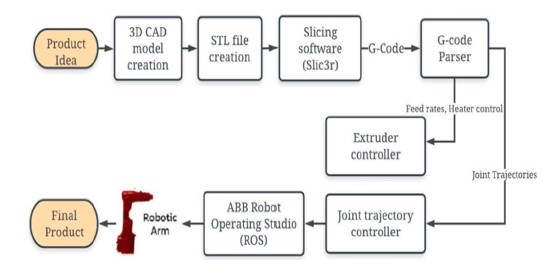
\includegraphics[scale=0.5]{figuras/flujo_trabajo_robot.jpg}
    \caption{Flujo de trabajo con un manipulador robótico incorporado \cite{Kubalak2016}}
    \label{fig:flujo_trabajo_robot}
\end{figure}

Los modelos más básicos se fundamentan en la implementación de una librería de código para el cálculo de trayectorias y el envío de mensajes. Estos modelos ya establecieron los tres agentes fundamentales en este tipo de sistemas: un controlador local para el cálculo de trayectorias, otro específico para el manipulador robótico y una interfaz que adaptase los mensajes entre ambos.

Uno de los sistemas más detallados fue el propuesto por Huang et al. \cite{Huang_2003}, mostrado en la Figura \ref{fig:modelo_arquitectura_antiguo}. Este sistema se caracteriza por establecer un modelo sencillo y robusto que además incorporaba una nueva capa de control supervisado por computador. El trabajo de Santos et al. \cite{Santos_2005} estaba más enfocado en un desarrollo de software portable y fácil de programar con varios lenguajes. No obstante ya propuso utilizar en desarrollos futuros comunicaciones industriales (protocolo Ethernet en concreto) para introducir una capa de procesamiento de datos distribuida, como puede verse en la Figura \ref{fig:arquitectura_ethernet}.

    \begin{figure}[h!]
        \centering
         \begin{subfigure}[h]{0.45\linewidth} 
            \centering
            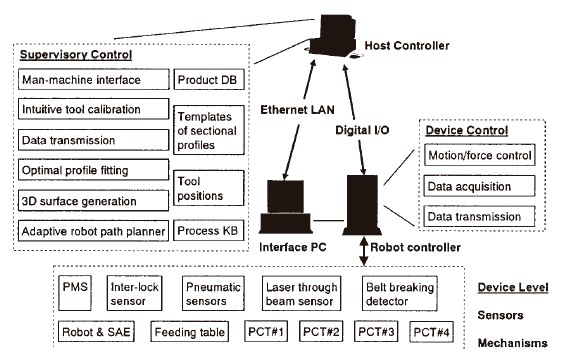
\includegraphics[scale=0.50]{figuras/modelo_arquitectura_antiguo.jpg}
            \caption{Modelo de tres agentes \cite{Huang_2003}}
            \label{fig:modelo_arquitectura_antiguo}
        \end{subfigure}
        \begin{subfigure}[h]{0.45\linewidth} 
            \centering
            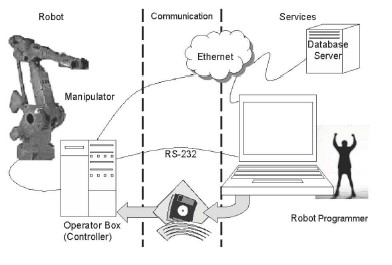
\includegraphics[scale=0.65]{figuras/arquitectura_ethernet.jpg}
            \caption{Comunicaciones por Ethernet \cite{Santos_2005}}
            \label{fig:arquitectura_ethernet}
        \end{subfigure}
        \caption{Primeras arquitecturas informáticas}
    \end{figure}

El paso del tiempo y el desarrollo de la microelectrónica favoreció la introducción de los sensores y actuadores con los que cuentan los robots industriales hoy en día. Con estos dispositivos se ha podido desarrollar modificaciones más especializadas de los primeros modelos de arquitectura informática, especialmente en el campo de la calibración y aprendizaje del robot.  

Del lado de la calibración se tiene parte del trabajo de Villagrossi et al. \cite{Villagrossi2018}. La Figura \ref{fig:arqutiectura_control_villagrossi} muestra cómo toma un ordenador industrial para implementar su triple bucle de control y se sirve de una capa de comunicaciones por protocolo \acrshort{TCP/IP} para enviar las acciones correctoras a un controlador diseñado específicamente para el robot. Como muestra la Figura \ref{fig:arquitectura_zheng_capas}, la propuesta de Zheng et al. \cite{Zheng_2022} se caracteriza por establecer cuatro capas de software especializadas en la interacción con el operador humano, el análisis de datos, la programación de movimientos y una interfaz de comunicaciones con ayuda del \acrshort{PLC} del robot.

    \begin{figure}[h!]
        \centering
         \begin{subfigure}[h]{0.45\linewidth} 
            \centering
            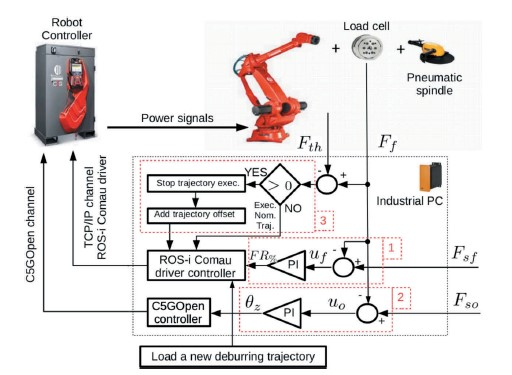
\includegraphics[scale=0.35]{figuras/arqutiectura_control_villagrossi.jpg}
            \caption{Ordenador y comunicaciones \acrshort{TCP/IP} \cite{Villagrossi2018}}
            \label{fig:arqutiectura_control_villagrossi}
        \end{subfigure}
        \begin{subfigure}[h]{0.45\linewidth} 
            \centering
            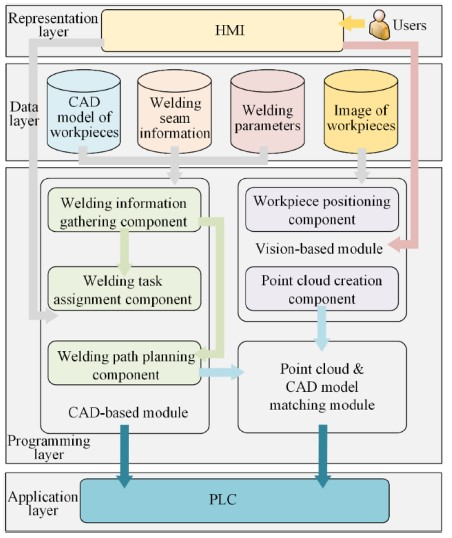
\includegraphics[scale=0.25]{figuras/arquitectura_zheng_capas.jpg}
            \caption{Capas especializadas de software \cite{Zheng_2022}}
            \label{fig:arquitectura_zheng_capas}
        \end{subfigure}
        \caption{Arquitecturas especializadas en calibración}
    \end{figure}

Por su parte, el aprendizaje también representa desarrollos interesantes en arquitecturas de estaciones robotizadas, especialmente el de tipo offline. Este tipo de arquitecturas se ven reforzadas por el uso de entornos de programación robótica como puede ser el caso de \acrshort{ROS}. 

El trabajo de Wei et al.\cite{Wei_2018} expone un diseño de arquitectura que minimiza la programación directa entre hombre y máquina. Este modelo se muestra en la Figura \ref{fig:arquitectura_Wei_2018} en forma de flujo de trabajo con capas de diferente nivel de abstracción. Se caracteriza por ser compatible con sistemas operativos de uso general y el uso de programación con \acrshort{ROS} para definir unos bloques de funciones específicas (como puede ser el control de un AGV, detección de humanos en el entorno o un generador de trayectorias de mecanizado a partir de un modelo \acrshort{CAD}). Los bloques función cuentan con su propia interfaz, por lo que una de las limitaciones que se trató de solventar fue la definición de unas capas intermedias de mensajes.

\begin{figure}[h!]
    \centering
    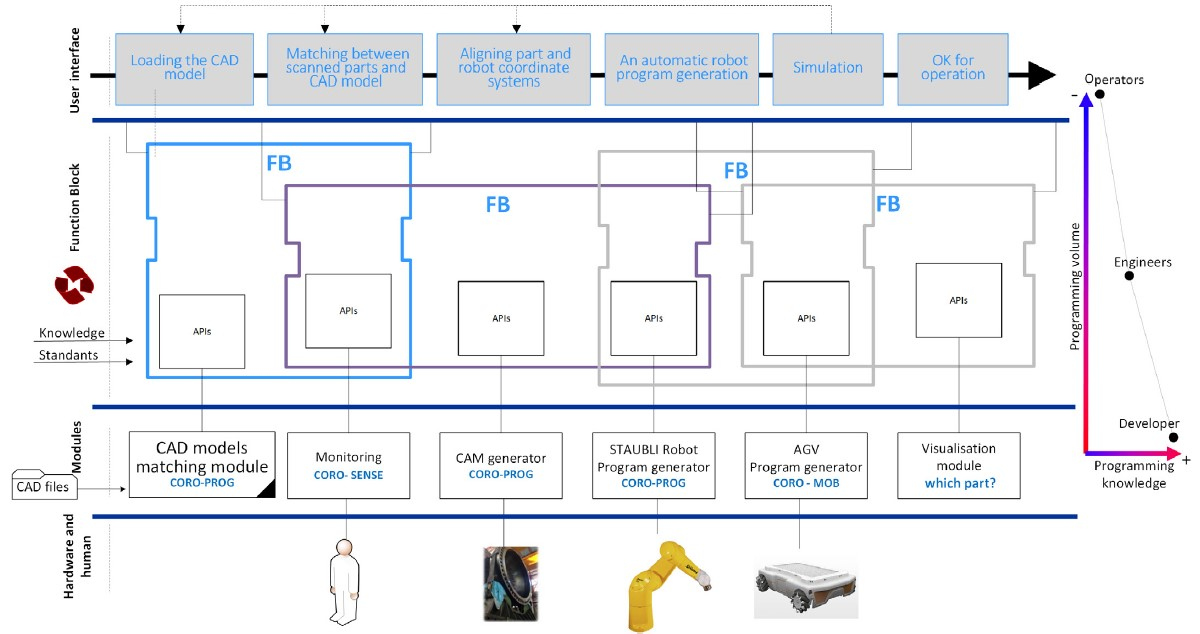
\includegraphics[scale=0.35]{figuras/arquitectura_Wei_2018.jpg}
    \caption{Flujo de trabajo y arquitectura por capas de \acrshort{ROS} especializadas \cite{Wei_2018}}
    \label{fig:arquitectura_Wei_2018}
\end{figure}

Otra de las grandes limitaciones en las arquitecturas informáticas enfocadas en el aprendizaje online son los métodos de comprobación de las trayectorias generadas. Verl et al. \cite{Verl_2019} expone en su revisión que muchos sistemas que basan su cálculo de trayectorias en modelos de inteligencia artificial que minimizan un parámetro de error. Como puede observarse en el procedimiento representado por la Figura \ref{fig:correccion_trayectorias_offline}, la compensación de errores suele darse en la etapa de cálculo de trayectoria o justo antes de enviarla al manipulador robótico, a modo de revisión previa. En otras palabras, a priori no existe un método definido para comprobar la exactitud durante la fabricación del resultado final y se deja a la propia pericia y experiencia del operario.

\begin{figure}[h!]
    \centering
    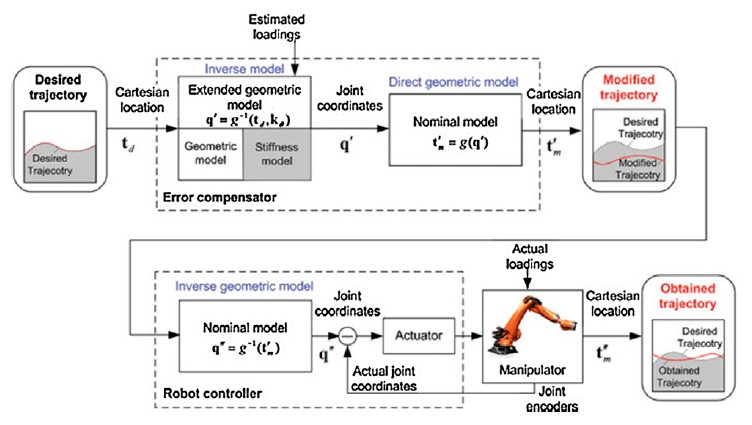
\includegraphics[scale=0.5]{figuras/correccion_trayectorias_offline.jpg}
    \caption{Corrección offline de trayectorias \cite{Klimchik2014}}
    \label{fig:correccion_trayectorias_offline}
\end{figure}

Cada vez más arquitecturas informáticas de este tipo integran sistemas de corrección de trayectoria durante la ejecución, para minimizar los errores del producto final. Esta solución necesita que la estación se adapte rápidamente a las necesidades de fabricación, por lo que se recurre a soluciones basadas en bloques de control individuales que se comunican entre sí. La Figura \ref{fig:arquitectura_controlador_celda} es un ejemplo de este paradigma. En ella se establecen varios bloques función con su propia programación y algoritmos de control, no obstante todos ellos se comunican entre sí a través de una interfaz de mensajes común. Esta interfaz es la definida por un elemento central que hace de controlador general de la estación (en color salmón en la Figura \ref{fig:arquitectura_controlador_celda}).

\begin{figure}[h!]
    \centering
    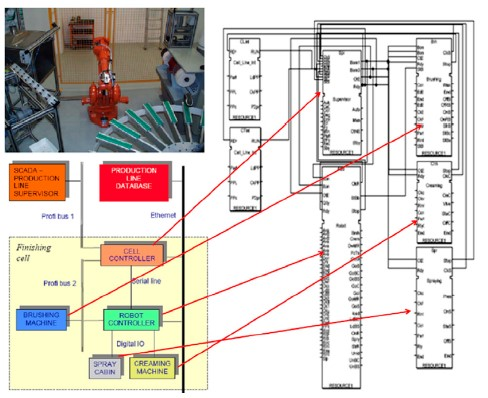
\includegraphics[scale=0.5]{figuras/arquitectura_controlador_celda.jpg}
    \caption{Arquitectura con controlador central de celda \cite{Verl_2019}}
    \label{fig:arquitectura_controlador_celda}
\end{figure}


\subsection{Fabricación aditiva no planar (\acrshort{NPAM})}
La implementación de dispositivos robóticos con más de tres \acrshort{DOF} en procesos de fabricación aditiva  supone una mayor libertad en el diseño y desarrollo de nuevas geometrías. Este enfoque se ve favorecido gracias a que un mayor número de grados de libertad permite configuraciones cinemáticas más complejas, pudiendo llegar a puntos que con otras tecnologías estaban restringidos para el equipo de diseño de la pieza. El manipulador robótico y los equipos hardware anexos pueden asumir la responsabilidad de calcular nuevas trayectorias y movimientos de deposición de forma independiente y modular.

Es decir, el proceso incrementa su eficiencia y se abre la puerta a que se aborden nuevas geometrías que puedan optimizar otros aspectos del proceso de fabricación como pueden ser configuraciones geométricas, empleo de material, uso de soportes de impresión o mejora de las propiedades mecánicas. Un ejemplo de aplicación directa de este enfoque son los procesos de fabricación \acrshort{NPAM}

La \acrshort{NPAM} es una técnica avanzada de fabricación aditiva que se caracteriza por permitir la impresión de geometrías de capa con curvatura. Es decir, las piezas resultantes de este proceso no se ven sometidas a las restricciones típicas de la \acrshort{AM} basada en la deposición de material en capas planas horizontales, como son:

\begin{itemize}
    \item \textbf{Direcciones privilegiadas:} Los elementos fabricados mediante impresión 3D tradicional se han realizado mediante la acumulación de capas planas. Esta disposición favorece un comportamiento anisótropo muy restringido, esto es, existen direcciones muy claras en las que el producto final es más resistente ante un esfuerzo concreto que otras. En el caso de la fabricación aditiva mediante capas planas convencionales, estas direcciones suelen ser trazados rectos y paralelos al plano de impresión.
    
    \item \textbf{Adhesión entre capas:} En los procesos \acrshort{AM} siempre se busca obtener un resultado final lo más macizo posible. Esto implica que las capas de deposición deben evitar el deslizamiento entre ellas, ya que puede afectar a la rugosidad, acabados y comportamiento mecánico de la pieza. Nótese en la figura \ref{fig:comportamiento_anisotropo3} cómo la deposición en capas poco adheridas favorece una anisotropía de la pieza en la dirección longitudinal, es decir, la perpendicular a las capas.

    \item \textbf{Movimiento tridimensional:} Las técnicas \acrshort{AM} tradicionales solamente pueden desplazarse en movimientos que resulten de una combinación de las direcciones cartesianas XYZ. Por otro lado, las piezas diseñadas y enviadas a imprimir cuentan siempre con partes con una parametrización cartesiana compleja que obliga a emplear soportes cuando existen voladizos. Un ejemplo puede verse en la figura \ref{fig:fdm_soporte_desventaja}.
\end{itemize}

   \begin{figure}[h!]
        \begin{subfigure}[h!]{0.45\linewidth} 
            \centering
            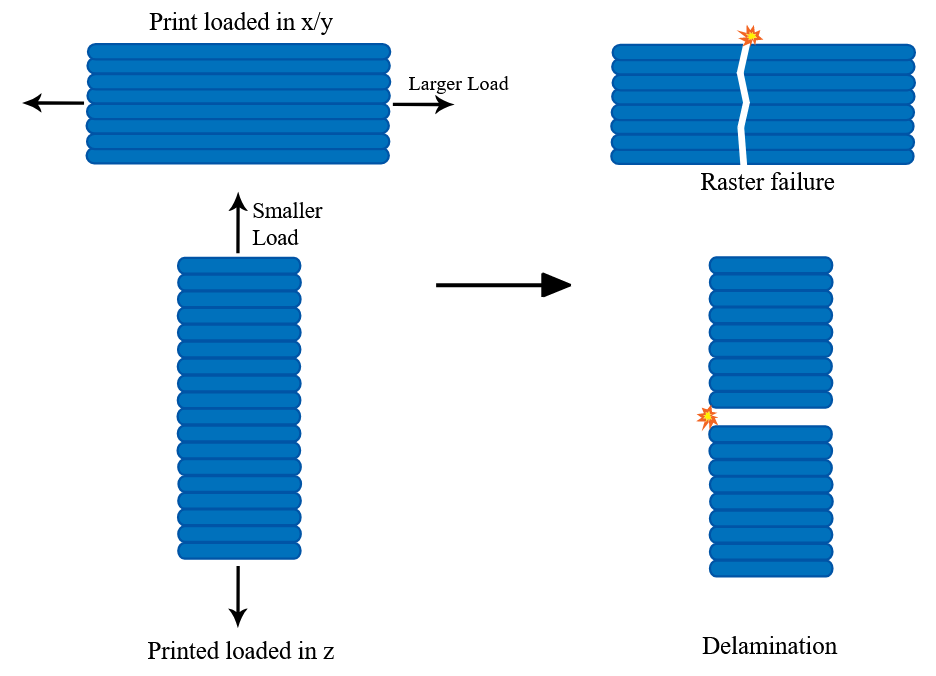
\includegraphics[scale=0.25]{figuras/comportamiento_anisotropo3.png}
            \caption{Comportamiento anisótropo entre capas\cite{web_fdm_properties}}
            \label{fig:comportamiento_anisotropo3}
        \end{subfigure}
        \begin{subfigure}[h!]{0.45\linewidth} 
            \centering
            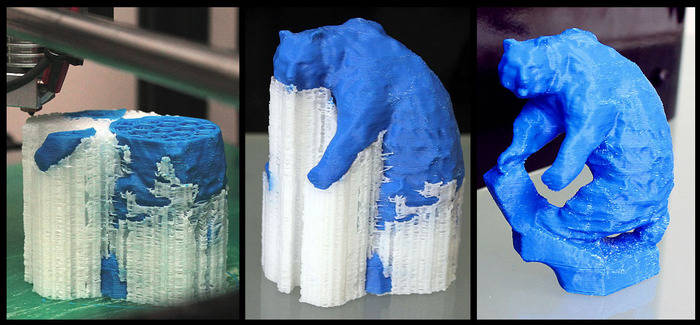
\includegraphics[scale=0.25]{figuras/fdm_soporte_desventaja.jpg}
            \caption{Uso de soportes para piezas con voladizos}
            \label{fig:fdm_soporte_desventaja}
        \end{subfigure}
        \caption{Limitaciones de la \acrshort{AM} tradicional}
    \end{figure}

La \acrshort{NPAM} solventa estas problemáticas y supone ventajas como:
\begin{itemize}
    \item \textbf{Complejidad geométrica:} Se puede imprimir sobre capas con curvatura directamente. De este modo se pueden conseguir buenos resultados en figuras basadas en estructuras curvas o con una gran cantidad de voladizos, cosa que en modelos más tradicionales de fabricación aditiva resultaría imposible.

    \item \textbf{Mayor capacidad de personalización:} Se pueden trazar trayectorias curvas más complejas, este aspecto puede ser de gran utilidad para la fabricación de dispositivos para necesidades específicas. Como ejemplo, en la figura \ref{fig: am_geometria_anatomica} se muestra cómo se utiliza un proceso de este tipo para poder imprimir capas de tejido sobre modelos biológicos.
    
     \begin{figure}[h!]
         \centering
         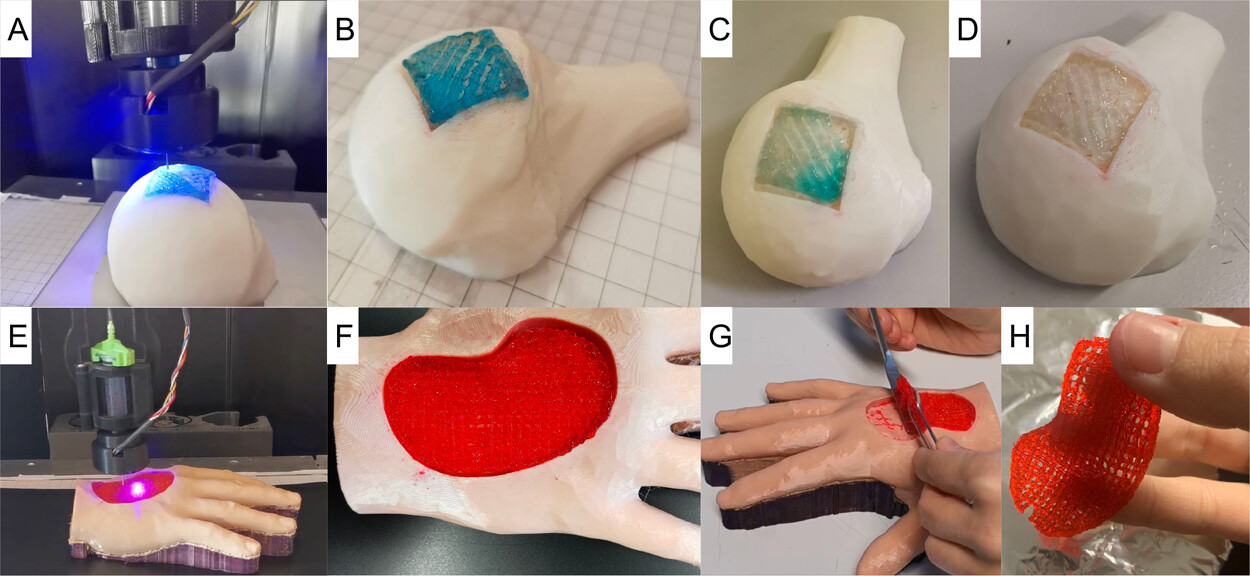
\includegraphics[scale=0.5]{figuras/am_geometria_anatomica.jpeg}
         \caption{Impresión \acrshort{NPAM} sobre modelos humanos \cite{Fortunato_2023}}
         \label{fig: am_geometria_anatomica}
     \end{figure}

    \item \textbf{Mejora de propiedades mecánicas:} La posibilidad de seleccionar impresiones en multitud de direcciones y tipos de capas permite reducir la anisotropía del resultado final, aumentando su resistencia a tracción y fatiga. En otras palabras, se orienta la dirección de anisotropía de forma favorable a los casos de carga en servicio de la pieza deseada. La figura \ref{fig:am_ensayos_resistencia_npam} muestra la comparativa entre una pieza modelo impresa por capas planas y otra mediante capas curvas.

    \begin{figure}[h!]
        \centering
        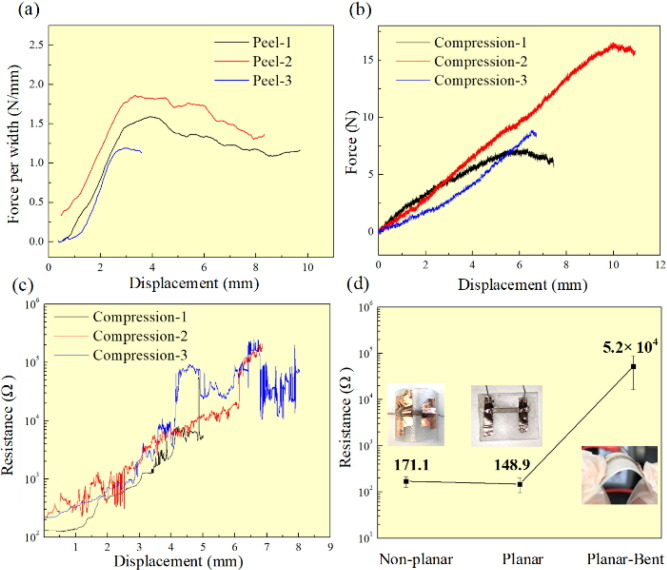
\includegraphics[scale=0.3]{figuras/am_ensayos_resistencia_npam.jpg}
        \caption{Mejora de propiedades mecánicas en productos NPAM \cite{Jiang_2021}}
        \label{fig:am_ensayos_resistencia_npam}
    \end{figure}

    \item \textbf{Eficiencia aumentada:} La \acrshort{NPAM} no solamente aporta resultados más personalizados y con propiedades mecánicas superiores, si no que también es efectiva para la introducción de economías de escala en grandes cantidades de piezas. Todo a causa de que se reduce la impresión de voladizos, se favorece el reciclaje de los soportes de impresión y se ahorra material. Este enfoque resulta altamente provechoso ya no solo desde una perspectiva económica, si no también desde una medioambiental \cite{Cendrero_2021}.
\end{itemize}

\section{Limitaciones y motivación}
En esta sección se definen las limitaciones del estado de la ciencia hasta el momento, indicando aquellos que pueden resultar de mayor interés de cara a efectuar una aplicación industrial práctica y adaptable al entorno de trabajo. En una segunda parte, se definirán las limitaciones de mayor impacto y que sirven también de motivación para el proyecto final.

\subsection{Limitaciones} \label{seccion: Limitaciones}
El presente proyecto trabaja con un robot colaborativo que sirve como herramienta principal de una estación \acrshort{NPAM}. A diferencia de muchos ejemplos observados en la literatura -que se basan en utilizar una boquilla extrusora móvil integrada con el cabezal del robot- aquí se plantea restringir los grados de libertad asociados a la boquilla extrusora en pro del desplazamiento de la cama de impresión. 

\subsubsection*{Arquitecturas de estación}
\hypertarget{Arquitecturas de estación}{}
\bookmark[level=subsubsection,dest=Arquitecturas de estación]{Arquitecturas de estación}

Las arquitecturas informáticas de estaciones robotizadas deben ser capaces de realizar varias tareas complejas como son el cálculo de trayectoria, la compensación de errores, la toma de datos en directo o la gestión de información en tiempo real. Por lo que las soluciones suelen tender hacia modelos compuestos por varios controladores especializados. Cada controlador deberá comunicarse con los demás a través de una serie de mensajes comunes bien entre una pareja específica o con ayuda de un bloque global de gestión.

No existe un modelo único, si no que se establece a partir de una base y trata de adaptarse a las necesidades de fabricación aditiva. En concreto, en el caso de aquellas estaciones que incorporan elementos de fabricación \acrshort{NPAM} cobran una especial relevancia las tareas de cálculo de desplazamientos y corrección de trayectorias, paro los que se prefiere introducir su propio esquema de comunicaciones.

Sin embargo, una arquitectura de comunicaciones no puede limitarse a optimizar las tareas más relevantes dentro de cada proceso, si no que también debe crear un entorno común al resto de agentes que la integran. Es decir, se debe disponer de un controlador que pueda gestionar toda esta información.

El paso del tiempo ha hecho que se definan lenguajes que sirven para diseñar mensajes de diferentes tipos, pero todavía queda en responsabilidad del ingeniero definir la información más relevante y cómo ha de tratarse.


\subsubsection*{Entorno de trabajo}
\hypertarget{Entorno de trabajo}{}
\bookmark[level=subsubsection,dest=Entorno de trabajo]{Entorno de trabajo}

Para llevar las operaciones de calibración y aprendizaje, los robots comerciales suelen implementar su propia solución en forma de entorno de trabajo o \textit{framework}. De cara a la operación del robot, esta estrategia supone ventajas como reducir de la curva de aprendizaje del manejo del equipo, acelerar la puesta en marcha de proyectos o aprovechar al máximo el hardware del equipo. De cara a aplicaciones que requieren de una mayor flexibilidad, esta dependencia del entorno del fabricante puede dificultar la integración del manipulador con otros sistemas y componentes externos, limitar la portabilidad y escalado del código o reducir la vida útil del equipo a unas aplicaciones muy concretas.

Ante estos desafíos, en el año 2007 surge la iniciativa \acrshort{ROS} \cite{ROS_web}\cite{ROS_wiki} (figura \ref{fig:ros_aplicaciones}), una suite\footnote{Conjunto de archivos y aplicaciones informáticas de instalación única que realizan diferentes funciones} de código abierto para facilitar la programación y control de robots. De este modo se puede decir que las características \cite{Saavera_2023} que definen a \acrshort{ROS} como entorno de trabajo son:

\begin{enumerate}
    \item Gestión de paquetes
    \item Intercambio de mensajes entre procesos
    \item Abstracción de hardware y control de dispositivos a bajo nivel
    \item Computación distribuida
    \item Soporte para varios lenguajes de programación (Python y C++)
    \item Reutilización de software 
    \item Realización ágil de pruebas
    \item Estándares de comunicación comunes
\end{enumerate}
    
El transcurso del tiempo hizo que comenzaran a salir a la luz algunas de las limitaciones de \acrshort{ROS} como entorno. Unas de las críticas más comunes son su falta de soporte para entornos distribuidos en tiempo real, su capacidad limitada para operar grandes volúmenes de datos o la imposibilidad de incluir programación entre varios lenguajes dentro de un mismo proyecto \cite{desventajas_ROS_webpage}\cite{ROS_vs_ROS2_webpage}. Estas limitaciones pueden ser una fuente de error en aplicaciones complejas como conducción autónoma \cite{Perez-Gil_2021}\cite{hachem_2023} o robótica industrial de precisión \cite{Nabissi_2023}. 

Para abordar estas deficiencias, surgió ROS2 \cite{ROS2_web}\cite{ROS2_docu_humble} (figura \ref{fig:ros2-humble-small}) como una nueva versión que conserva muchas de las ventajas de su antecesor, pero también introduce mejoras y soluciones importantes. Algunos ejemplos son la integración de un soporte multiplataforma entre Python y C++, una interfaz nativa para sistemas distribuidos en tiempo real, una arquitectura software más modular o la solución de problemas de escalabilidad y rendimiento.
    
\begin{figure}[h!]
    \begin{subfigure}[h!]{0.45\linewidth} 
        \centering
        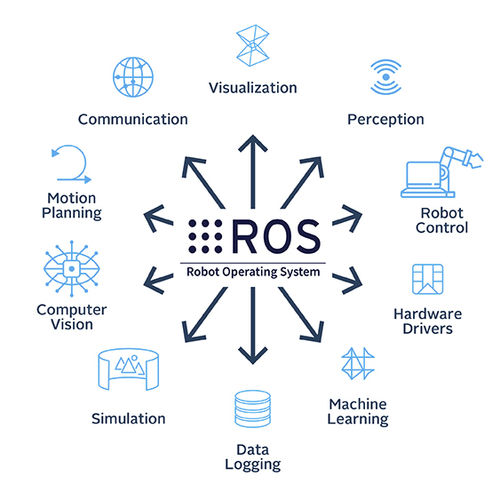
\includegraphics[scale=0.20]{figuras/ros_aplicaciones.jpg}
        \caption{Framework de \acrshort{ROS}}
        \label{fig:ros_aplicaciones}
    \end{subfigure}
    \begin{subfigure}[h!]{0.45\linewidth} 
        \centering
        
\includegraphics[scale=1.6]{figuras/ros2-humble-small.png}
        \caption{Versión de ROS2 de este proyecto \cite{ROS2_docu_humble}}
        \label{fig:ros2-humble-small}
    \end{subfigure}
    \caption{Limitaciones de la \acrshort{AM} tradicional}
\end{figure}

\subsection{Motivación del proyecto}
Siguiendo la línea descrita por la sección \ref{seccion: Limitaciones}, se ha visto que existen multitud de métodos de calibración extrínseca para una estación de fabricación robotizada. En todos ellos se ha visto que la tendencia actual apunta hacia la inclusión de procesos de calibración que además incluyan un sistema de aprendizaje offline. Esto es, que también se simulen rápidamente las operaciones planteadas para el robot. 

Es fundamental establecer un proceso de preparación de la estación de trabajo en el que se pueda obtener de forma eficaz la definición de sus sistemas de referencia fundamentales. En otras palabras, se necesita operar grandes cantidades de datos de forma distribuida que permitan caracterizar geométrica y mecánicamente la mesa de trabajo, la herramienta empleada o las trayectorias a efectuar por el robot.

Como se ha visto anteriormente, la inclusión de únicamente las herramientas proporcionadas por el fabricante del robot no resulta suficiente para este tipo de aplicaciones. Por lo que el sistema de preparación debe contar con parámetros en tiempo real como la inclinación de la mesa, la presencia de elementos móviles o la temperatura del material depositado.

En este proyecto se propone un sistema de preparación de la estación de fabricación que integre estas funciones dentro de una interfaz amigable para el usuario y que pueda sintetizar un flujo de trabajo sencillo y modularizado. Para ello se definirá una estrategia de calibración offline de la estación, mientras se evalúan una serie de parámetros en tiempo real como puede ser la temperatura de la cama de impresión. 

Para solventar la capacidad de gestión de datos del robot -que resulta insuficiente para el objetivo de la estación- se plantea la integración de una arquitectura en \acrshort{ROS}2 con un computador externo efectuando otras tareas de forma simultánea. La introducción de ROS2 como entorno de trabajo frente a ROS, tiene la intención de servir como base para futuros desarrollos en los que se puedan definir (1) nuevas herramientas de cálculo de trayectorias usando la programación cruzada entre Python y C++, (2) una modularización de tareas por parte del robot y (3) la posibilidad de establecer comunicaciones en el futuro con elementos de una arquitectura de comunicaciones distribuida.

\section{Marco del proyecto} \label{section:  marco del proyecto}
Este proyecto se ha desarrollado dentro de un entorno multidisciplinar más grande. El objetivo a largo plazo de este equipo es el diseño y construcción de una estación de fabricación aditiva robotizada centrada en los procesos \acrshort{NPAM}. El proceso abarcado se puede definir a través de tres etapas:
\begin{enumerate}
    \item \textbf{Planificación de producto:} Es la parte correspondiente al diseño de piezas que pasarán a la estación de fabricación. En ella se busca implementar un algoritmo de slicing automatizado \cite{paper_Q1_Alvaro_Adrian} que permita obtener un conjunto de puntos cartesianos en el espacio que definan la pieza resultante final. Amparo Sancho en su trabajo anterior \cite{TFM_SanchoAmparo} estableció una primera versión de este proceso y es la que se ha usado como referencia principal.
    \item \textbf{Preparación de estación:} Esta etapa comprende las operaciones de calibración del brazo robótico empleado y calentamiento del extrusor y la cama de impresión. En esta fase del proceso general es donde se encuentra ubicado este proyecto.
    \item \textbf{Operación de manufactura:} Es la fase final del proceso. En ella se da luz verde para que una vez la cama y el extrusor se encuentren a las temperaturas deseadas, el brazo robótico comience a efectuar la trayectoria calculada para obtener el producto definido en la fase de planificación.
\end{enumerate}

Los materiales aportados para el diseño y montaje de la estación han sido aportados por el grupo de \href{https://fabricacion.industriales.upm.es/}{Ingeniería de Fabricación} de la \href{https://www.industriales.upm.es/}{ETSII-UPM}. Dentro de todos los componentes utilizados destaca el robot UR10 ubicado en el laboratorio del grupo junto a una mesa de trabajo especialmente diseñada para su operación.

\begin{figure}[h!]
    \centering
    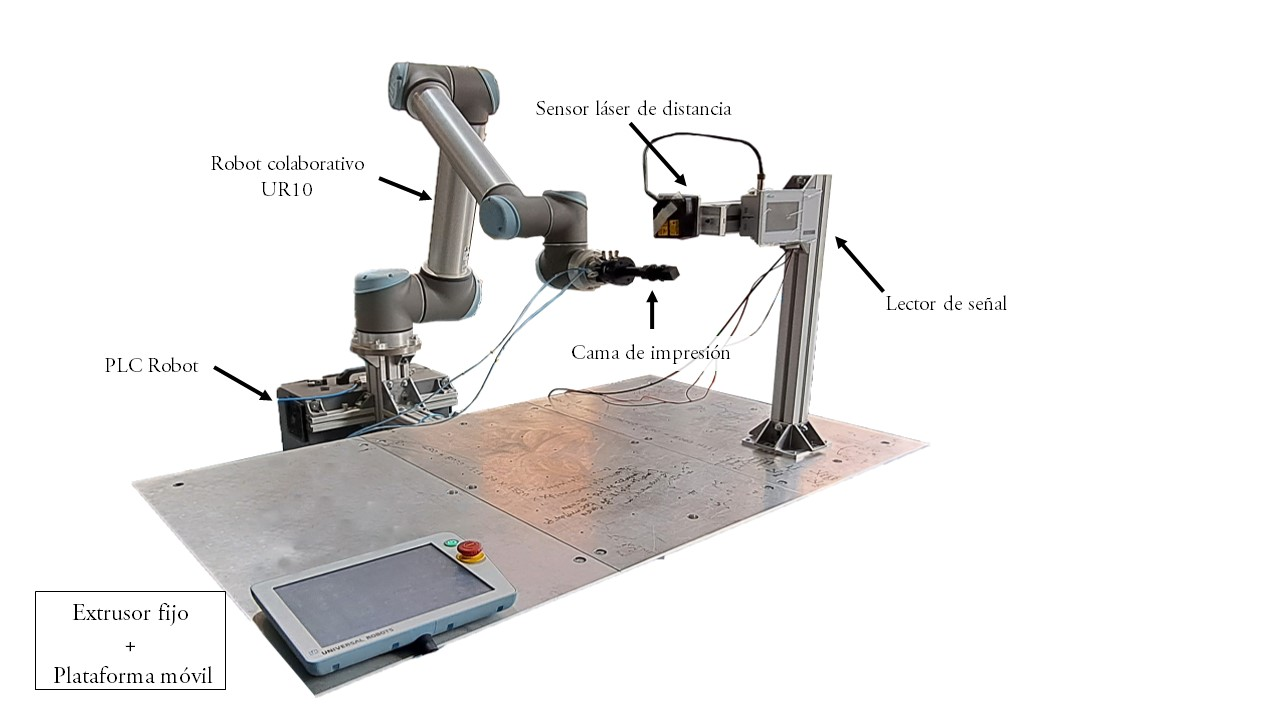
\includegraphics[scale=0.30]{figuras/estacion_NPAM_sin_estruxor.JPG}
    \caption{Versión inicial de la estación}
    \label{fig: estacion_NPAM_sin_estruxor}
\end{figure}

Se desea que la estación tenga la cama acoplada al \acrshort{TCP} y el extrusor se encuentre ubicado en una posición fija con la finalidad de asegurar que el material extruído se deposite en la dirección de la gravedad. Esta configuración también es útil para ampliar el diseño de plataformas de impresión personalizadas, de modo que sea posible aprovechar más los \acrshort{DOF} proporcionados por el manipulador robótico. De cara a soluciones más convencionales, esta configuración resulta ventajosa para evitar introducir grados de libertad extra relacionados con la configuración de la mesa o el soporte de la estación. 

La Figura \ref{fig: estacion_NPAM_sin_estruxor} muestra una versión inicial de la estación \acrshort{NPAM} y se sitúa aproximadamente por el mes de Octubre de 2023. Esta versión incluye un sensor láser para tomar medidas de calibración de la cama del robot y ha sido utilizada en trabajos de fin de titulación previos \cite{TFM_SanchoAmparo} \cite{TFM_Lu}.

La cama cuenta con su propio diseño realizado por Iñaki Echepare \cite{TFM_IñakiEchepare} y se caracteriza por contar con un cartucho calefactor en su interior que puede activarse a conectándolo a un circuito electrónico. El soporte para el extrusor ha sido diseñado por Adrián Martínez. 

Tanto los datos de temperatura de la cama de impresión como del extrusor, deben retransmitirse de forma continuada a una unidad de control. En el caso de la temperatura de la cama, los mensajes y el bucle de control han sido definidos en colaboración con Irene Rodríguez.

Este macroproyecto integra labores variadas de cálculos cinemáticos, conocimientos de automatización, comunicaciones industriales, electrónica o ensayos de mecánica de materiales. Es decir, tiene un alcance transversal y necesita la colaboración de equipos multidisciplinares. En otras palabras y como punto adicional de este trabajo, se ha establecido un marco de coordinación entre algunos de los equipos partícipes en el diseño y construcción de la estación robotizada. En concreto se han establecido las interfaces de comunicación entre arquitecturas software y de operación hardware, así como también se ha creado un \href{\linkrepositorio}{repositorio} donde se ubica un manual de conocimiento básico del proyecto en forma de wiki  \cite{repo_github_TFM_MiguelLerinAlonso}.

La Figura \ref{fig:areas_macroproyecto} muestra las diferentes áreas que conforman este macroproyecto\footnote{Una versión con los nombres de los alumnos involucrados en cada tarea se dispone en la Figura \ref{fig:marco proyecto tareas y autor} del apéndice \ref{cap: anexo marco proyecto}.}, se marcan en color rojo aquellas en las que este trabajo tiene un papel principal. Estas tareas entran dentro de tres campos principales: la arquitectura informática de la máquina, la planificación de procesos y generación de trayectorias; y la preparación de de procesos. Las tareas efectuadas dentro del área de arquitectura informática fueron aquellas relacionadas con la creación de una interfaz de usuario de ROS2 para el manejo y operación de la estación. Las correspondientes a la planificación de procesos y generación de trayectorias de buscaban definir un nuevo flujo de trabajo para la estación e integrarlo con los equipos ya existentes y los de nuevo desarrollo. Finalmente, se realizaba una tarea de calibración del robot dentro del área de preparación de procesos.

\begin{figure}[h!]
    \centering
    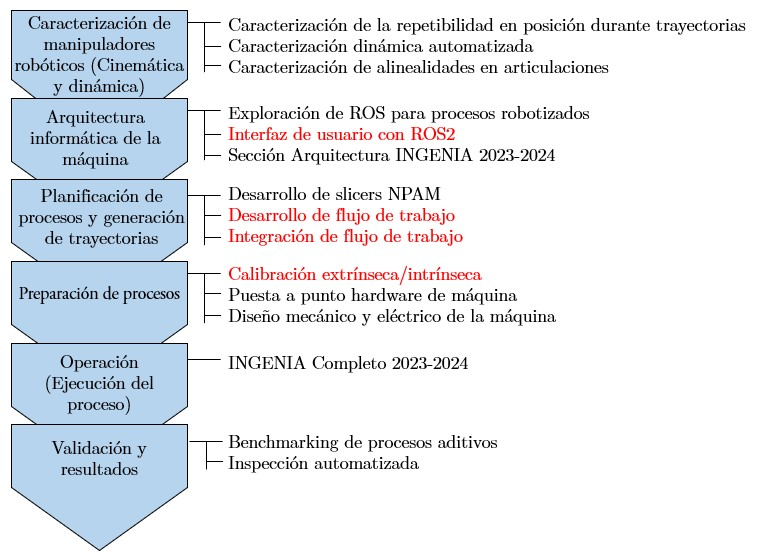
\includegraphics[scale=0.65]{figuras/marco_proyecto_solo_tareas_v2.jpg}
    \caption{Áreas del macroproyecto en el que se integra este trabajo}
    \label{fig:areas_macroproyecto}
\end{figure}

La Figura \ref{fig:ambitos_coordinacion} establece una representación visual de los ámbitos de coordinación llevados durante este proyecto. Como puede observarse, a parte del presente trabajo existen cinco equipos especializados que colaboran activamente entre sí. Los equipos están formados por otros alumnos que se encuentran trabajando en sus respectivos trabajos de fin de titulación y alumnos del curso 2023-2024 de la asignatura \href{http://fabricacion.industriales.upm.es/2022/09/06/asignatura-ingenia-diseno-de-estacion-colaborativa-4-0/}{INGENIA Diseño de sistemas inteligentes con robots y AGV} \cite{web_INGENIA}. La labor de dichos equipos y su conexión con el presente proyecto se describen en las siguientes lineas:

\begin{itemize}
    \item \textbf{Generación de trayectorias:} Equipo responsable de programación del software de slicing empleado para el procesamiento de modelos \acrshort{CAD} que desean ser impresos. Este equipo aporta al proyecto un archivo CSV en el que se encuentran definidos el conjunto de puntos asociados a un sistema referencia que debe recorrer el manipulador robótico. Es decir, aporta los datos de entrada para el sistema de cálculo configuraciones cinemáticas del robot UR.
    \item \textbf{\acrshort{DfAM}:} Este equipo es el responsable de plantear y evaluar aquellas técnicas de diseño mecánico que pueden ser de mejor resultado para los requisitos de la estación. Deben tener en cuenta el tipo de producto que se desea fabricar a través del proceso \acrshort{NPAM} y trabajar junto a la sección de Generación de trayectorias para hallar el procedimiento óptimo de orientación y fabricación de la pieza objetivo. Es decir, los componentes de este equipo se encargan de valorar la integración de otras tecnologías en el resultado final como pueden ser metodologías multimaterial o con optimización topológica.
    \item \textbf{Diseño mecánico y eléctrico:} Los integrantes de esta sección han sido responsables de la elaboración del soporte que aloja el extrusor de material. Esta sección está en contacto constante con \acrshort{DfAM} para valorar la energía y flujo de material que demanda la pieza resultado del proceso \acrshort{NPAM}. Sigue el proceder con la sección de Actuadores máquina para especificar la alimentación eléctrica que deben proveer a los actuadores de la máquina.
    \item \textbf{Actuadores máquina:} Está sección es la encargada de establecer integrar y establecer los bucles de control que relacionan a los actuadores de la estación \acrshort{NPAM} robotizada. Esta labor la hacen en colaboración con el equipo de Arquitectura para mejorar el tratamiento de los sensores y actuadores, y siguen las directrices indicadas por el diseño de la arquitectura informática realizada en este trabajo. Los equipos de sensorizado y actuación más relevantes para sus integrantes han sido el control de temperatura asociado a la cama de impresión y la regulación del extrusor de material en cuanto a flujo de alimentación y modelado térmico.
    \item \textbf{Arquitectura:} Son los responsables de la definición de movimientos del robot UR a través de un conjunto de aplicaciones software que deben también monitorizar sus variables internas. Reciben el conjunto de puntos definido por el software de slicing de la sección de Generación de trayectorias y se encuentran en conversaciones continuadas con el equipo de actuadores máquinas para definir el conjunto de mensajes entre equipos y su tratamiento. También colaboran en este proyecto en labores de optimización de código, pruebas de ejecución en tiempo real o la definición del espacio de trabajo virtualizado.
\end{itemize}

\begin{figure}[h!]
    \centering
    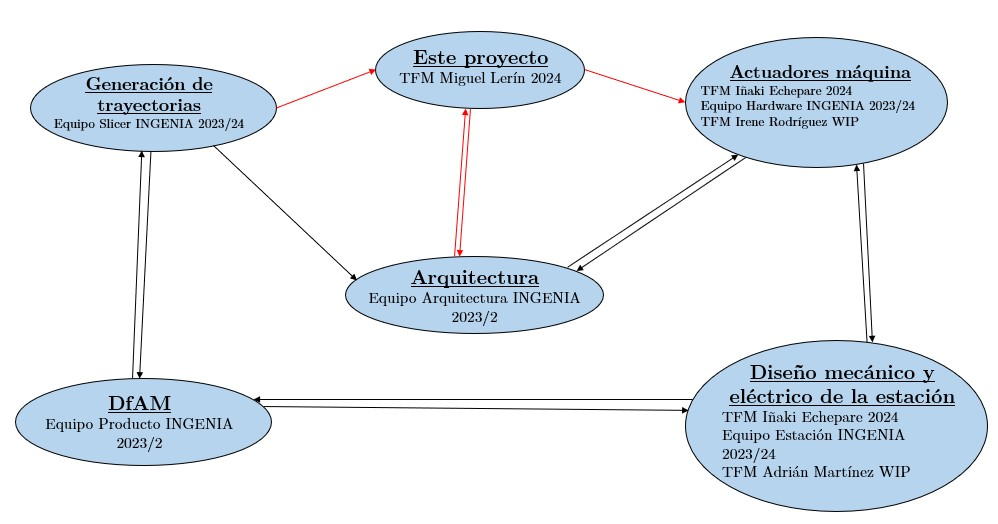
\includegraphics[scale=0.6]{figuras/ambitos_coordinacion_1_esquema_v2.jpg}
    \caption{Ámbitos de coordinación llevados durante la ejecución del trabajo}
    \label{fig:ambitos_coordinacion}
\end{figure}

\phantom{Este texto no se verá, pero ocupará espacio. Lo uso para que la figura de los ámbitos de coordinación quede al comienzo de la página}
\chapter{Objetivos y estructura de la memoria} \label{cap: objetivos}
\section{Objetivo del trabajo}
El objetivo principal de este trabajo es la implementación de un sistema de control basado en ROS2 que permita preparar fácilmente una estación robotizada de fabricación aditiva.

El trabajo puede dividirse en cuatro partes fundamentales:
\begin{enumerate}
    \item \textbf{Diseño de arquitectura de control:} Se definen los actores principales del flujo de trabajo de la estación \acrshort{NPAM} indicando el tipo de mensajes trabajados y las actuaciones de control que deben efectuarse.
    \item \textbf{Sistema de toma de datos:} Elaborar un sistema de toma de datos genérico que permita conocer en todo momento las variables de control del robot de la estación.
    \item \textbf{Ejecución automática de trayectorias:} Implementar un algoritmo de cálculo y generación de trayectorias a partir de los modelos \acrshort{CAD}.
    \item \textbf{Calentamiento de la plataforma de impresión:} Desarrollar un controlador sencillo que permita calentar la plataforma de impresión y regular su temperatura para mantenerse fiel al valor consigna que le comande el computador central al comienzo de la etapa de preparación del proceso \acrshort{AM}.
\end{enumerate}

\section{Estructura de la memoria}
La estructura del trabajo se compone de un total de 10 capítulos. Los primeros se plantean como una introducción al problema y a los conocimientos técnicos necesarios para la comprensión del proyecto y del resto de la memoria. Los siguientes cuatro capítulos tienen una carga más técnica y se han redactado con la intención de describir cada subobjetivo del trabajo de forma independiente. Esto es, cada uno cuenta con su propia introducción al problema, descripción de la metodología seguida y balance de resultados y conclusiones. Los últimos tres capítulos corresponden a las conclusiones finales del proyecto, la descripción de la planificación y presupuestos seguidos y un análisis del impacto del proyecto en diferentes dimensiones.

Los siguientes puntos describen más detalladamente el contenido de cada capítulo de la memoria:

\begin{itemize}
    \item En el capítulo \ref{cap: introduccion}  se hace una definición sencilla de \acrshort{AM} mencionando sus orígenes y algunas de sus aplicaciones más novedosas. Del mismo modo, también se comentan los últimos avances del campo resaltando aquellos que sirven de especial interés para la motivación del presente proyecto. Después de hablar de la motivación del proyecto, el capítulo finaliza presentando el marco de trabajo físico, el entorno del laboratorio del grupo de \href{https://fabricacion.industriales.upm.es/}{Ingeniería de Fabricación} de la ETSII-UPM.

    \item En el capítulo \ref{cap: objetivos} se definen el objetivo principal del proyecto y se indica la subdivisión que se ha hecho en objetivos más pequeños para favorecer su correcto seguimiento. También se describe la estructura de la memoria indicando el contenido de cada capítulo.

    \item En el capítulo \ref{cap: fundamento_teorico} se presentan aquellos conocimientos necesarios para comprender el alcance del trabajo y su funcionamiento. Es decir, se presentará al robot utilizado, los conceptos esenciales de \acrshort{ROS}, el modelo cinemático empleado y las herramientas de software que han permitido el cálculo y ejecución de las trayectorias deseadas. También se presentarán otros equipos físicos de importancia para este proyecto como la cama de impresión \acrshort{NPAM} o el sensor de desplazamiento láser entre otros.

    \item El capítulo \ref{cap: diseno_arquitectura} describe la arquitectura de control integrada dentro de la estación del presente proyecto. La metodología seguida se divide en dos partes: una primera que define aquellos requisitos técnicos esenciales que debe implementar el sistema, y una segunda en la que se describe el desarrollo obtenido. El capítulo finaliza presentando un caso de uso como ejemplo y además comenta las ventajas y posibles mejoras del modelo de arquitectura implementado.

    \item El capítulo \ref{cap:lectura_datos} presenta el sistema de lectura de datos de ejecución del manipulador robótico de la estación y de los dispositivos que dependen de él como es el caso del sensor de distancia láser. Se comienza identificando las señales de mayor importancia y su naturaleza, posteriormente se describe el funcionamiento del sistema basado en ROS2 responsable de su muestreo. Finalmente, a modo de resultados se presentará al menos un caso de uso para cada variable de interés y se procederá a evaluar las ventajas y limitaciones del paquete desarrollado.

    \item En el capítulo \ref{cap: trayectorias} se describe el proceso de desarrollo del sistema de cálculo y ejecución de trayectorias a partir de la matriz de puntos obtenida del proceso de slicing. Esto se hace definiendo tres objetivos de menor nivel referentes a la construcción de un entorno de planificación offline con capacidad de detección de colisiones con elementos reales, el desarrollo de un sistema de cálculo y ejecución de trayectorias robóticas no planares para el cobot; y un control de velocidad de ejecución de movimiento. El capítulo cierra presentando las validaciones realizadas para cada objetivo y comentando las ventajas y principales limitaciones del sistema y las herramientas empleadas.

    \item El capítulo \ref{cap: control_temperatura} expone el desarrollo del sistema de control automática de temperatura de la plataforma de impresión. Se arranca definiendo un modelo propio de arquitectura de comunicaciones para este dispositivo en el que se favorezca la modularidad del conjunto de la estación. A continuación se procede a describir el modelo de control propuesto y se evalúa su desempeño en dos ensayos diferenciados. Finalmente se comenta las ventajas aportadas por la filosofía de diseño e implementación utilizadas y se resaltan las limitaciones del estado actual de dicho dispositivo.

    \item En el capítulo \ref{cap:discusion_conclusiones} se realiza una revisión de todos los objetivos de mayor y menor nivel planteados en este trabajo para, a continuación valorear las ventajas y limitaciones observadas durante la ejecución del proyecto. Finalmente se discutirá la conveniencia de dichas soluciones extrayendo un conjunto de conclusiones generales e indicando posibles líneas futuras de trabajo.

    \item El capítulo \ref{cap: planificacion_presupuesto}  es el referente a la planificación temporal del proyecto y el cálculo de su presupuesto de ejecución. Como sistemas de planificación se aborda un modelo de la planificación estratégica -que hace uso de herramientas como la \acrshort{EDP} y el diagrama Gantt- y un modelo de planificación ágil basado en la filosofía Kanban. 

    \item El capítulo \ref{cap:evaluacion_impactos} abarca un análisis integral del proyecto en cuatro apartados clave. En primer lugar, se evalúa el impacto social del proyecto, considerando su influencia en la comunidad y los posibles beneficios o desafíos que pueda generar. En segundo lugar, se examina el impacto económico, analizando los costos, ahorros y efectos financieros que el proyecto podría implicar. En tercer lugar, se valora el impacto medioambiental se destacan aquellos aspectos positivos y negativos para el entorno natural. Finalmente, se realiza un comentario de la contribución del proyecto a los Objetivos de Desarrollo Sostenible (ODS), identificando los objetivos específicos a los que apoya y cómo puede contribuir a su cumplimiento.
\end{itemize}
\chapter{Fundamento teórico y materiales empleados} \label{cap: fundamento_teorico}
En este capítulo se presentarán aquellos conceptos esenciales para comprender el funcionamiento de este proyecto. La intención de este capítulo es hacer una presentación sencilla y fácil de comprender de todos los actores involucrados, para una descripción más en detalle se ha elaborado a modo de apéndice una wiki disponible en el \href{\linkrepositorio}{repositorio de GitHub asociado} \cite{repo_github_TFM_MiguelLerinAlonso}. 

\section{Fundamento teórico}
\subsection{Robot colaborativo}
Un robot colaborativo (o \textit{cobot} en el argot especializado) es un tipo de robot industrial enfocado a trabajar de forma segura y eficiente siempre en compañía de operarios humanos. Es decir el robot y los operadores comparten un entorno físico real en el que interactúan mutuamente y donde debe prevalecer siempre la seguridad del operario. 

Los robots industriales comunes se diseñan para trabajar en tareas repetitivas de alta velocidad y precisión, es decir, resultan idóneos para operaciones especializadas. Estos robots también pueden sostener grandes cargas durante periodos prolongados de tiempo, motivo por el que siempre cuentan con una separación física entre su entorno y el operario como puede ser una barrera de seguridad. La programación de este tipo de robots a menudo viene definida por el fabricante en un entorno cerrado y enfocado a tareas sencillas. Estos motivos han hecho que se les considere equipos destinados a proyectos con tareas claramente definidas en las raramente existan variaciones respecto del modelo original. Es decir, se necesita disponer en todo momento de operarios e ingenieros especializados programando trayectorias in-situ, lo que supone una inversión en tiempo y costes a tener en cuenta.

Los robots colaborativos suponen una alternativa más segura para entornos donde se requiere programar varias tareas en poco tiempo. La premisa de este tipo de manipuladores es la flexibilidad dentro de su entorno físico. Es decir, pese a que se desplazan a velocidades menores que un robot convencional o su carga máxima es más limitada, su diseño ligero y compacto resulta perfecto para un trabajo mano a mano con el operario. Este enfoque permite que se realicen tareas versátiles que no impliquen un riesgo significativo.

En la Figura \ref{fig:comparativa_robots} se muestra una comparativa resumen de ambos equipos.
\begin{figure}[h!]
\centering
    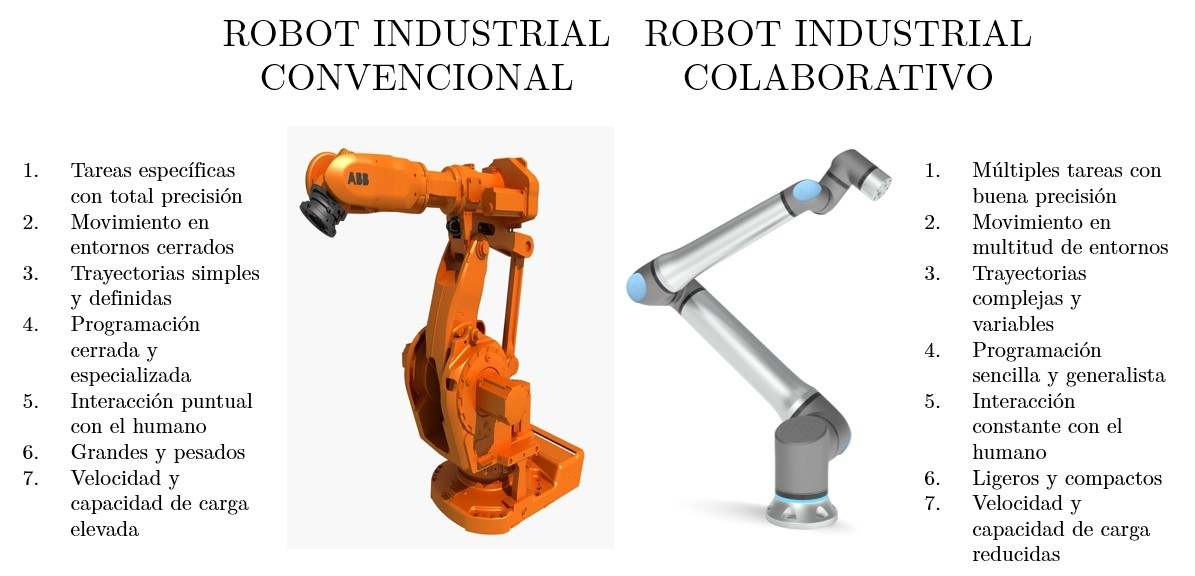
\includegraphics[scale=0.5]{figuras/comparativa_robots_v2.jpg}
    \caption{Comparativa de robots industriales}
    \label{fig:comparativa_robots}
\end{figure}

\subsubsection*{Cobot UR10}
En este trabajo se ha optado por emplear un robot colaborativo UR10 de la marca Universal Robots. Se ha considerado que este equipo resulta ideal para la iniciación en entornos de fabricación aditiva robotizada al poder operar con velocidades reducidas y permitir realizar multitud de iteraciones en poco tiempo. También se ha tenido en cuenta la necesidad de implementar correcciones rápidas de forma directa sin entrañar grandes riesgos para el usuario.

 Las características técnicas de este modelo se muestran en la tabla \ref{tab:caracteristicas_UR}. Existen parámetros cuyo valor es inherente a la unidad utilizada y tuvieron que medirse en el laboratorio en trabajos previos \cite{TFM_SanchoAmparo}.

\begin{table}[h!]
    \begin{subfigure}[h!]{0.45\textwidth}
        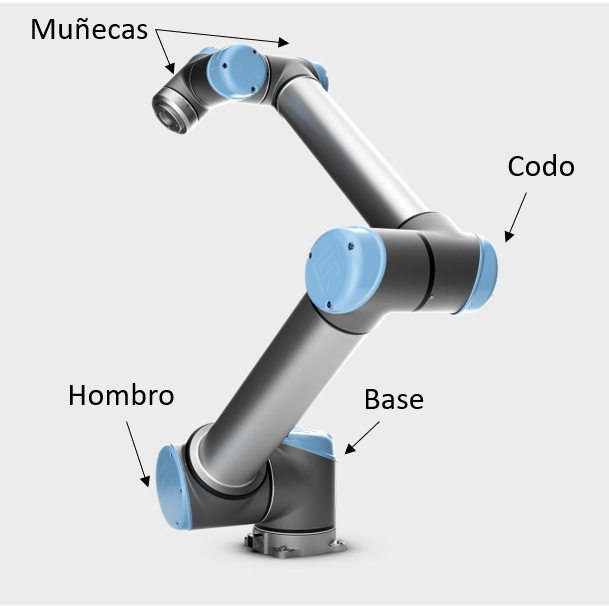
\includegraphics[scale=0.5]{figuras/articulaciones_UR.png}
        %%\caption{Articulaciones del UR}
        \label{fig:articulaciones_UR}
    \end{subfigure}
    \hfill
    \begin{subfigure}[h!]{0.7\textwidth}
        \begin{tabular}{|l|r|}
            \hline
            Carga máxima & 10 kg \\
            \hline
            Alcance máximo & 1300 mm \\
            \hline
            Giro de articulaciones & ± 360º \\
            \hline
            Grados de libertad & 6 \\
            \hline
            Huella & 190 mm \\
            \hline
            Temperatura de trabajo & 0-50 ºC \\
            \hline
            Repetibilidad & ± 0.1 mm \\
            \hline
            Error de trayectoria \footnote{Medido en el laboratorio} & ± 0,2 mm \\
            \hline
            Velocidad de giro de base y hombro & 120 º/s \\
            \hline
            Velocidad de giro de codo y muñeca & 180 º/s \\
            \hline
        \end{tabular}
        %%\caption{Valores característicos}
        \label{tab:caracteristicas_UR_tabla}
    \end{subfigure}
    \caption{Características del UR10 \cite{UR_Technical_Specs}}
    \label{tab:caracteristicas_UR}
\end{table}


\subsection{Cinemática del robot}
Es el campo de estudio del movimiento del robot y la posición de sus articulaciones. En este campo se tiene un especial interés no solamente en el conjunto de poses que le permiten alcanzar al robot un punto del espacio cartesiano, si no también en el comportamiento de sus sensores y actuadores con el transcurso del tiempo. 

No se tienen en cuenta las fuerzas y torques aplicados por el robot para mantener su posición o para manipular algún elemento. El acceso de estos parámetros suele estar únicamente abierto para el fabricante, lo que es de especial utilidad para enfocarse en la labor de cálculo y trazado de trayectorias por parte del usuario.

En el estudio de la cinemática, se ha de tomar siempre un punto de referencia que sirva para la definición de trayectorias, velocidades y aceleraciones que se desea efectuar. Normalmente se suele tomar como convenio el \acrshort{TCP} del robot (también llamado \textit{end-effector} en \href{https://hades.mech.northwestern.edu/images/7/7f/MR.pdf}{literatura especializada de referencia} \cite{Modern_Robotics}). La definición del \acrshort{TCP} pasa por efectuar una serie de transformaciones entre varios marcos de referencia utilizando herramientas matemáticas como las matrices de traslación-rotación (véase como ejemplo la expresión \ref{eq: Ejemplo_matriz_TR}). 

\begin{equation}
\begin{gathered}
    \textbf{TR} =
    \begin{bmatrix}
    1 & 0 & 0 & p_x \\
    0 & 1 & 0 & p_y \\
    0 & 0 & 1 & p_z \\
    0 & 0 & 0 & 1 
    \end{bmatrix}
    \label{eq: Ejemplo_matriz_TR}
\end{gathered}
\end{equation}
\begin{equation*}
\text{Ejemplo de matriz de traslación-rotación}
\end{equation*}

La cinemática busca relacionar dos interpretaciones del espacio con las que debe operar el robot en todo momento:
\begin{itemize}
    \item \textbf{Interpretación cartesiana:} Es la definición de un punto en el espacio a través de tres coordenadas posición (XYZ normalmente) y tres de rotación (ángulos de Euler $\alpha\beta\gamma$)\cite{euler_agle_formulas}. No existe un convenio claro para definir las rotaciones, por lo que existen otras herramientas igualmente válidas como los ángulos aeronáuticos de Tait-Bryan \textit{Roll, Pitch y Yaw} \cite{quaternions_applications} o los \textit{cuaterniones} \cite{Quaternion_Algebra}. Para todas estas herramientas ya existen métodos de conversión bien definidos y fiables \cite{quaternions_and_Euler_Angles}.

    \item \textbf{Interpretación articular:} Es la medida del desplazamiento que debe efectuar el robot para situar su \acrshort{TCP} en el punto destino. Este desplazamiento se mide en referencia al movimiento que debe efectuar cada articulación.
\end{itemize}

Para establecer la relación entre ambas representaciones del espacio, se utilizan las ecuaciones de la cinemática directa y la cinemática inversa. La Figura \ref{fig: comparacion cinematicas} muestra a modo conceptual el enfoque de cada cinemática.

\begin{itemize}
    \item \textbf{Cinemática directa:} Define la posición y orientación del \acrshort{TCP} del robot en el espacio cartesiano a partir de una configuración articular concreta. 

    \item \textbf{Cinemática inversa:} Define los valores de desplazamientos articulares que debe tomar el robot para situar su \acrshort{TCP} en unas posiciones cartesianas de entrada. La solución de este problema no es única y se aborda mediante dos posibles métodos:
        \begin{enumerate}
            \item \textbf{Método geométrico:} Es el más conveniente para robots con un número reducido de \acrshort{DOF}. El enfoque que se suele tomar es el de plantear las ecuaciones de la cinemática directa y despejar de ahí las variables articulares en función de las cartesianas.
            \item \textbf{Cambio entre sistemas de referencia:} Se emplean diferentes métodos numéricos para obtener la matriz de traslación-rotación que define relaciona diferentes sistemas de referencia ubicados en el \acrshort{TCP}, la base del robot, la herramienta e incluso entre los diferentes eslabones. Este método es el más adecuado para un gran número de \acrshort{DOF} por ser fácil de programar y permitir implementar distintos algoritmos de cálculo.
        \end{enumerate}
\end{itemize}

\begin{figure}[h!]
    \centering
    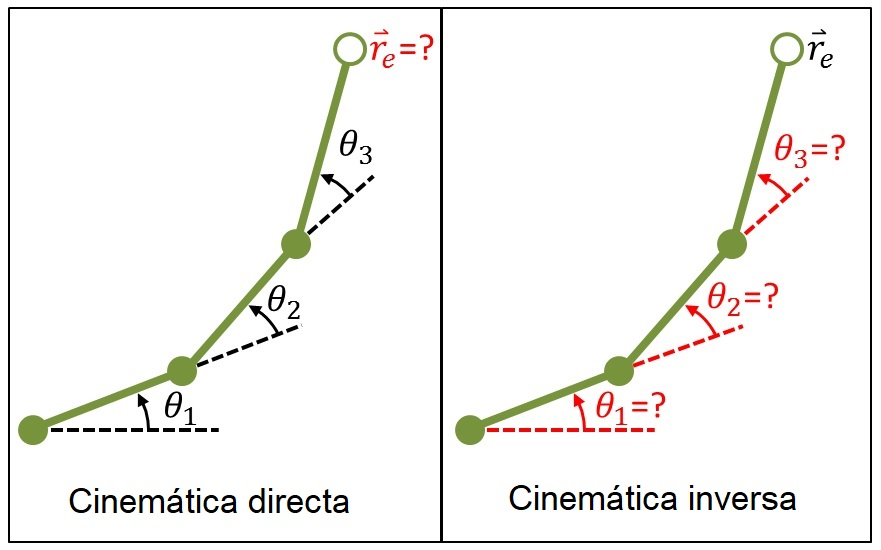
\includegraphics[scale=0.4]{figuras/ik_vs_fk.jpg}
    \caption{Comparación entre cinemáticas \cite{Najam_R_Syed_kinematics_webpage}}
    \label{fig: comparacion cinematicas}
\end{figure}

\subsection{ROS2} \label{section: presentacion ROS2}
ROS2 es un entorno de trabajo software proveniente de \acrshort{ROS}. Se trata un conjunto de librerías e implementaciones software que permite el desarrollo de aplicaciones robóticas a partir de código escrito en lenguajes más generalistas como C++ o Python. De este modo, el usuario puede prescindir de un conocimiento extenso en las implementaciones software del propio robot y centrarse en otras labores como el control de sensores o el cálculo de trayectorias. 

ROS2 sigue los principios fundamentales de su antecesor, pero también implementa ciertas mejoras como:
\begin{itemize}
    \item Soporte multiplataforma entre diferentes lenguajes de programación
    \item Interfaz nativa para sistemas operativos corridos en tiempo real
    \item Mayor modularización entre nodos y paquetes
    \item Implementación de mensajes más flexibles y con comunicación directa ente nodos gracias a protocolos \acrshort{DDS}
\end{itemize}

En este trabajo se ha implementado un sistema de trazado e implementación de trayectorias basado en ROS2 en el robot UR10. Este sistema además es capaz de enviar diversos mensajes entre diferentes nodos y comunicarse con otros equipos de la estación. 

Las siguientes líneas buscan explicar las principales diferencias en el entorno construido con ROS2 frente a uno que implemente \acrshort{ROS}. Si es necesario consultar conceptos básicos de programación en este tipo de entorno, se recomienda consultar la documentación oficial \cite{ROS2_docu_humble} o la \href{\linkrepositorio}{wiki del  repositorio de este proyecto} \cite{repo_github_TFM_MiguelLerinAlonso}.

\begin{itemize}
    \item \textbf{Estructura básica}\\
    \acrshort{ROS} es un entorno de programación robotizada centralizado, es decir, es necesario definir un nodo maestro del que dependerán el resto de nodos. En ROS2 no es necesario definir un único nodo que sirva como base de la jerarquía, el sistema prima la modularización de código. 

    En ROS2, cada vez que se invoca un nuevo nodo en la red, éste es el responsable de avisar al resto de su presencia y de establecer las comunicaciones pertinentes con el resto de módulos. La Figura \ref{fig:Comparacion_ros_ros2} muestra una comparativa entre la estructura de archivos de un proyecto en ROS o otro en ROS2.
    
    \item \textbf{Comunicación entre nodos}\\
    Siguiendo la línea anterior, la capa de transporte de mensajes entre nodos también se ha visto modificada. ROS utilizaba una versión del protocolo \acrshort{TCP/IP} -conocida como TCPROS- que se había modificado de forma específica para cada tipo de comunicación entre nodos. Este enfoque traía problemas de compatibilidad y escalamiento entre tareas, reduciendo la ejecución y compilación del código en el largo plazo o en sistemas operativos en tiempo real.

    Para solventar esta problemática se optó por implementar un \textit{framework} de arquitectura publicador/suscriptor que sirviese como base para escalafones de un mayor nivel de abstracción como cliente/servidor o acción/cliente. Este \textit{framework} se llama \acrshort{DDS} \cite{ROS2_DDS} y se caracteriza por su prioridad en la calidad del mensaje. Es decir, se define un mensaje básico que puede ser interpretado por cualquier objeto de ROS2 y posteriormente se pueden añadir nuevos atributos accesibles al resto de nodos.
    
    \item \textbf{Sistema de compilado}\\
    Cualquier proyecto compilado necesita de un sistema que (1) elabore los ejecutables de forma automática y (2) pueda enlazar las distintas dependencias entre clases y librerías. ROS utiliza Catkin y resulta ideal para proyectos jerarquizados en los que es necesario definir un nodo principal desde el que dependen todas las funcionalidades. No obstante, al ser un sistema que construye archivos de compilación individual -como CMake \cite{documentacion_CMake}, en el que se basa-, Catkin no permite el la compilación entre varias plataformas, por lo que no resulta una buena opción en caso de integrar varias librerías escritas en Python, Java o C++.

    Por su parte Ros1 utiliza \textit{colcon}. Colcon pretende ser más modular y flexible extendiendo la estructura del proyecto gracias a la implementación de dependencias mediante ficheros \acrshort{YAML}. El uso de este tipo de ficheros resulta común a multitud de lenguajes y es más sencillo para el intérprete humano. De este modo se compila un único proyecto que integre diversos paquetes escritos en varios lenguajes en cuestión de segundos.
\end{itemize}

\begin{figure}[h!]
    \centering
    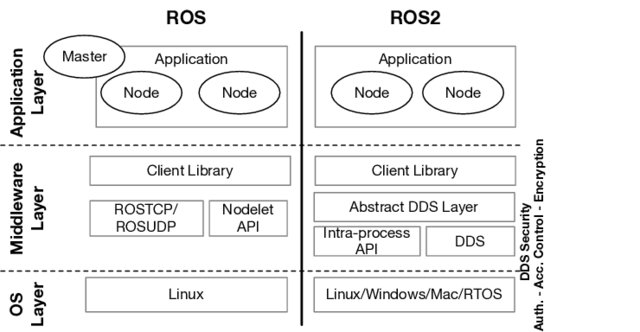
\includegraphics[scale=1.25]{figuras/Comparacion_ros_ros2.jpg}
    \caption{Comparativa entre capas software de ROS y ROS2 \cite{Mazzeo_2020}}
    \label{fig:Comparacion_ros_ros2}
\end{figure}


\subsection{RVIZ}
RViz \cite{guia_RViz} es una herramienta de visualización tridimensional dentro del ecosistema de ROS2. Permite a los desarrolladores y usuarios visualizar y analizar datos relacionados con robots de manera interactiva y en tiempo real. 

Una de sus principales ventajas radica en su capacidad para mostrar modelos 3D de robots basados en archivos \acrshort{URDF} \cite{web_defincion_URDF}, lo que facilita la comprensión de la estructura y la configuración del robot. Además, RViz ofrece una amplia gama de herramientas y accesorios que permiten personalizar la visualización según las necesidades específicas del usuario, desde representación de sensores y actuadores hasta la planificación de trayectorias o la simulación de robots en entornos virtuales.

Las herramientas RViz más empleadas en este trabajo han sido aquellas relacionadas con:
\begin{itemize}
    \item Virtualizar un entorno de trabajo real para implementar un modelo de cálculo de trayectorias que evite colisiones.
    \item Simulación de trayectorias y corrección de errores
    \item Descripción del robot mediante archivo \acrshort{URDF}
    \item Definir sistemas de coordenadas relativos entre diferentes componentes del robot
\end{itemize}

La Figura \ref{fig:entorno_virtual_rviz} muestra el entorno de trabajo de este proyecto virtualizado con ayuda de Rviz. Nótese que de forma análoga a la Figura \ref{fig: estacion_NPAM_sin_estruxor} se han incluido otros elementos complementarios al robot como la mesa de operación o el soporte para el sensor láser.

\begin{figure}[h!]
    \centering
    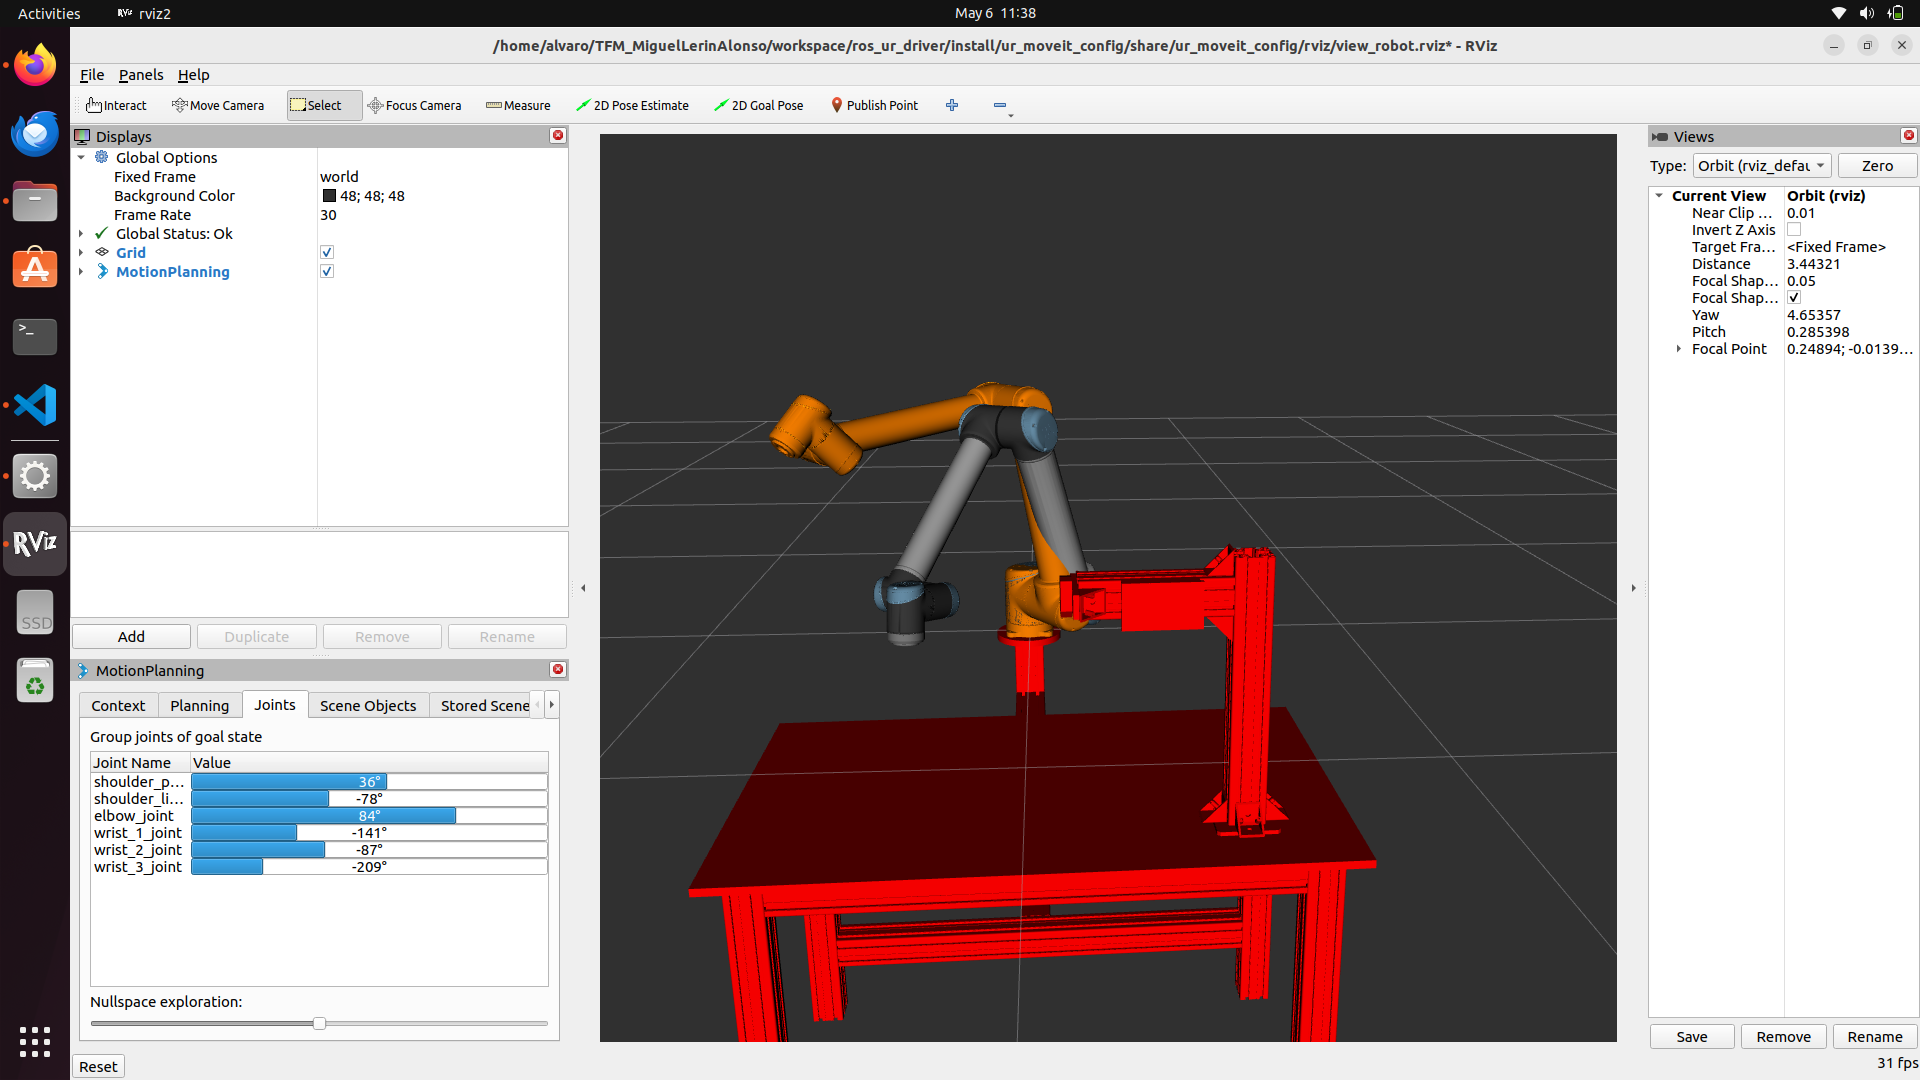
\includegraphics[scale=0.15]{figuras/entorno_virtual_rviz.png}
    \caption{Virutalización del entorno de trabajo de proyecto en RViz}
    \label{fig:entorno_virtual_rviz}
\end{figure}

\subsection{Moveit}
MoveIt \cite{moveit_documentacion} es un conjunto de herramientas de planificación y control de movimiento diseñado para robots en el ecosistema de ROS 2. La interfaz de este controlador busca ser fácil de usar y altamente flexible, lo que permite definir y ejecutar fácilmente tareas de planificación de movimiento para una amplia variedad de aplicaciones robóticas. Sus principales ventajas radican en su capacidad para integrarse con robots de diferentes configuraciones y cinemáticas, gracias a su soporte para modelos \acrshort{URDF} y su amplia compatibilidad con una variedad de controladores y plataformas. Todo ello pudiéndose hacer tanto en un entorno real como en uno simulado.

Una de las ventajas más destacadas de MoveIt en ROS2 es su capacidad para proporcionar una solución completa de planificación y control de movimiento que abarca desde la simulación hasta la ejecución en el mundo real. Esto permite a los usuarios desarrollar y probar algoritmos de planificación (también llamados \textit{solvers}) en entornos virtuales -como RViz- antes de implementarlos en robots reales. 

La misión de los solvers es proponer un conjunto de posiciones, velocidades, aceleraciones y esfuerzos articulares en el robot calculados a partir de un conjunto de valores semilla. Los valores semilla se definen como posiciones y orientaciones en el espacio cartesiano, dejando al controlador la propuesta de una solución optimizada para el trazado suave de la solución. A esta solución calculada por el solver, se le pueden introducir diferentes restricciones relativas al espacio de trabajo o la velocidad del movimiento.

Por comodidad, es usual asociar la trayectoria de entrada al solver con un sistema de referencia relacionado con un punto característico del robot como puede ser el \acrshort{TCP} o una de sus muñecas. En este trabajo se ha optado por referenciar todas las trayectorias de entrada a un punto asociado a la muñeca número 3 del UR por simplicidad geométrica. También se puede implementar una nueva definición en el controlador para otra articulación o un sistema asociado a un punto del espacio.

\subsection{Programación en Python}
Anteriormente, para desarrollar proyectos en \acrshort{ROS} era necesario utilizar únicamente un lenguaje de programación durante todo su periodo de vida. Este lenguaje de programación solía ser C++ cuando era necesario implementar soluciones que demandasen gran capacidad de cálculo (como la ejecución de trayectorias) y Python para casos en los que se necesitaba definir un conjunto de interfaces entre varios  nodos.

La ausencia de programación en varias plataformas para un mismo proyecto, impedía en muchos casos definir un conjunto de mensajes y algoritmos de cálculo óptimos para las tareas deseadas para el robot manipulador. Como se ha dicho anteriormente en la sección \ref{section: presentacion ROS2}, en ROS2 este inconveniente ha sido superado y es posible combinar ambos lenguajes dentro de una misma aplicación.

Las razones por las que se opta en este caso por implementar una programación con Python son:
\begin{enumerate}
    \item Gran parte de los paquetes y componentes en ROS2 tienen su equivalente en C++ y en Python. Se considera que están lo suficientemente evolucionados como para realizar un conjunto de modificaciones mínimas en su código.
    \item Python se considera un lenguaje de programación con una curva de aprendizaje menos acusada que C++. Es decir, el usuario puede aprender en poco tiempo la sintaxis del lenguaje y realizar su propias modificaciones en el código fuente original. Este enfoque se ha considerado más adecuado para usuarios no especializados en robótica, como pueden ser parte de los miembros partícipes del marco del proyecto (descrito en la sección \ref{section:  marco del proyecto}).
    \item Python es un lenguaje de alto nivel con una gran variedad de librerías. Estas librerías pueden integrarse de forma sencilla con los nodos de un ecosistema ROS2 y hacer uso de un paradigma \acrshort{POO}. Algunos ejemplos pueden ser las comunicaciones industriales mediante protocolos \acrshort{TCP/IP} o puerto serie, análisis de datos o creación de mensajes personalizados para comunicaciones entre nodos.
\end{enumerate}

C++ ofrece otras ventajas como que existen trabajos anteriores que pueden servir de referencia \cite{TFM_Lu}, se tiene un mayor control de la administración de la memoria y el tiempo de ejecución o que se ofrece una programación a más bajo nivel. No obstante, dado el enfoque transversal de este proyecto se ha optado por utilizar Python gracias a su mayor sencillez en aplicaciones experimentales, dejando la tarea de optimización de código para desarrollos futuros.

\section{Materiales y métodos}
\subsection{Sensor de medida de desplazamiento}
El cálculo de la trayectoria recae sobre una unidad de computación externa al robot que comunica la acción de ejecutarla. Comprobar que la boca extrusora se encuentra siempre a la misma distancia del punto de la cama de impresión especificada por la unidad central de la estación se emplea un sensor láser de distancia. 

Como primera iteración se ha utilizado un sensor SICK OD5-30W05 como el que se muestra en la siguiente figura. Sus características más relevantes vienen definidas en la Tabla \ref{tab:caracteristicas_sensor_sick_od5}.

\begin{table}[h!]
    \begin{subfigure}[h!]{0.45\textwidth}
        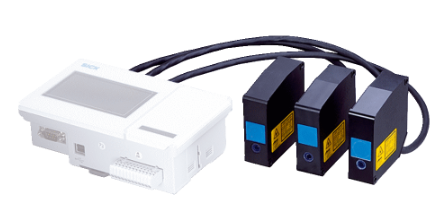
\includegraphics[scale=0.40]{figuras/sensor_SICK_1.png}
        %%\caption{Articulaciones del UR}
        \label{fig:articulaciones_UR}
    \end{subfigure}
    \hfill
    \begin{subfigure}[h!]{0.35\textwidth}
        \begin{tabular}{|l|r|}
            \hline
            Peso & 250 g \\
            \hline
            Rango de medida & 25-35 mm \\
            \hline
            Precisión de repetición & 0.2 $\mu$m \\
            \hline
            Tiempo de respuesta & 0.1-0.8 ms \\
            \hline
        \end{tabular}
        %%\caption{Valores característicos}
        \label{tab:caracteristicas_UR_tabla}
    \end{subfigure}
    \caption{Características del sensor SICK OD5-30W05 \cite{manuel_sensor_laser_sick_od5_30w05}}
    \label{tab:caracteristicas_sensor_sick_od5}
\end{table}

\subsection{Utillaje para el sensor de medida}
El sensor de medida se apoya sobre un utillaje diseñado en trabajos previos \cite{TFM_SanchoAmparo} y mejorado por compañeros del marco de trabajo. Este utillaje sirve como un soporte rígido y estable para ubicar otros elementos en el futuro como puede ser el extrusor de la estación robotizada \acrshort{NPAM}.

Este utillaje también ha servido de referencia para establecer restricciones en el cálculo de trayectorias a partir de su modelo \acrshort{CAD}. Se muestra como referencia la Figura \ref{fig:entorno_virtual_rviz}.

\subsection{Cama de impresión}
La cama de impresión utilizada en este proyecto ha sido elaborada como trabajo de fin de titulación de Iñaki Echepare \cite{TFM_IñakiEchepare}. Se ha utilizado como objetivo de trazado de trayectorias y comprobación de su exactitud. 

De forma análoga al utillaje para el sensor de medida, se implementa su modelo \acrshort{CAD} dentro del entorno virtualizado para establecer una nueva restricción en el cálculo de trayectorias. La Figura muestra una fotografía de la cama real con sus partes más importantes y a su lado su representación en el entorno virtual.

\begin{figure}[h!]
    \centering
    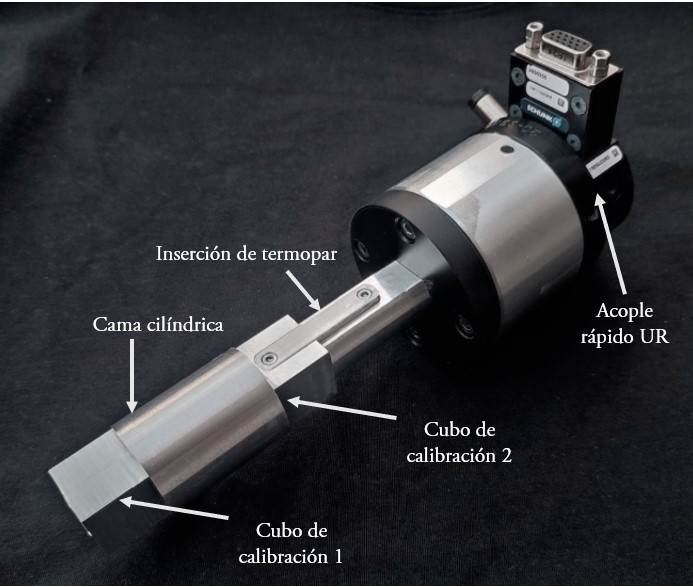
\includegraphics[scale=0.4]{figuras/cama_impresion_real.jpg}
    \label{fig:cama_impresion_real}
    \caption{Cama de impresión \cite{TFM_IñakiEchepare}}
\end{figure}

A continuación se describen algunas de las partes más importantes de la cama:

\begin{itemize}
    \item \textbf{Acople rápido UR:} Elemento de unión y sujeción de la cama al UR.
    \item \textbf{Cubos de calibración:} Dos geometrías diseñadas específicamente para establecer sistemas de referencia y puntos clave que permiten ubicar la cama en el espacio.
    \item \textbf{Cama:} Pieza de revolución (en este caso un cilindro simple) sobre la que se irá depositando el material extruído. En su interior dispone de un cartucho calefactor que proporciona el calor requerido para que el material solidifique de la forma deseada.
    \item \textbf{Inserción termopar:} Pletina de acceso a un dispositivo de medida de temperatura directa del cartucho calefactor.
\end{itemize}

\subsection{Controlador de temperatura}
Sistema de accionamiento del cartucho calefactor de la cama de impresión y lectura de su temperatura. Dispone de un termopar tipo K, un amplificador de la señal del termopar MAX6675 (características principales indicadas en la Tabla \ref{tab:caracteristicas_termopar}), un relé y una placa electrónica con controlador programble. El esquema eléctrico ha sido elaborado por Irene Rodríguez y ha contado con la revisión y control de ensayos del autor del presente proyecto.

\begin{table}[H]
    \centering
       \begin{tabular}{|l|r|}
            \hline
            Resolución & ±0.25 ºC\\
            \hline
            Rango de temperatura & 0-1024 ºCC \\
            \hline
            Tensión de alimentación & 0.3-6 V\\
            \hline
            Intensidad de salida & 50 mA \\
            \hline
            Constante de conversión & 41 $\mu$V/ºC \\
            \hline
            Temperatura de trabajo & 0-50 ºC \\
            \hline
        \end{tabular}
    \caption{Características del termopar MAX6675 \cite{manual_termopar_driver_max6675}}
    \label{tab:caracteristicas_termopar}
\end{table}


\chapter{Diseño de arquitectura de control}
\label{cap: diseno_arquitectura}

Este capítulo muestra el proceso de análisis, diseño e implementación de la arquitectura informática de control de la estación \acrshort{NPAM} robotizada. Se comenzará presentando el problema indicando aquellos aspectos considerados más importantes para los requisitos del sistema, para posteriormente describir el proceso de diseño que se ha seguido. Finalmente se presentará el desarrollo obtenido junto a un ejemplo de aplicación de una de sus funcionalidades. A partir del modelo de arquitectura presentado y el ejemplo de aplicación, se discutirán sus principales ventajas y aspectos por mejorar en nuevas iteraciones.

El código descrito en este capítulo se encuentra disponible en el repositorio GitHub del proyecto \cite{repo_github_TFM_MiguelLerinAlonso}. Los nodos de ROS2 que representan dichas tareas pertenecen al paquete \textit{rutine\_launcher}\footnote{Disponible en el direccionamiento: \textit{./workspace/ros\_ur\_driver/src/rutine\_launcher}}


\section{Introducción al problema}
La introducción de manipuladores robotizados en estaciones de fabricación aditiva supone el manejo de numerosas cantidades de datos y la abstracción de conceptos de robótica esenciales como pueden ser el cálculo de la cinemática, el muestreo de datos en directo del robot o la gestión del entorno de trabajo físico. Los robots colaborativos cuentan con su propia solución integrada dentro del manipulador, sin embargo, esta propuesta suele basarse en la gestión del \acrshort{PLC} acoplado al mismo y el conexionado a otras unidades. Es decir, no todo el mundo posee los conocimientos necesarios para poder operar dicho equipo y en ocasiones puede suponer un reto el conexionado de un nuevo sensor y la gestión de la información del robot.

Por estos motivos, se opta por integrar el manipulador robótico en un marco más grande donde existan unidades especializadas para cada una de la tareas antes mencionadas. Este marco suele enfocarse siempre a:

\begin{enumerate}
    \item Determinar unidades especializadas en las tareas clave del proceso de fabricación.
    \item Definir un conjunto de mensajes comunes a todos los elementos informáticos partícipes en el proceso.
    \item Construir un entorno modular que sea fácil de acceder y permita incorporar rápidamente nuevas funcionalidades.
\end{enumerate}

Teniendo en cuenta el marco de la estación con la que se está trabajando en este proyecto, la consecución de dichos objetivos debe pasar primero por una comprensión del flujo de trabajo que se desea implementar. A partir de dicho flujo será posible definir aquellas tareas más relevantes y asignar las responsabilidades que puede asumir el manipulador robótico por sí solo. Del mismo modo, dicha evaluación también servirá para identificar los puntos más críticos del proceso y evaluar si deben ser gestionados por otras unidades anexas.

\section{Metodología}
El procedimiento seguido en el este paquete de trabajo del proyecto puede dividirse en dos grandes etapas. La primera es la correspondiente a la definición de especificaciones y funcionalidades del proyecto, es decir, estudiar el flujo de trabajo del que parte la estación y definir sus requisitos y alcance del proyecto. La segunda etapa se da inmediatamente después de finalizar la primera y consta de la definición de todos los agentes automáticos que participan en el proceso de impresión \acrshort{NPAM} y cómo han de transmitirse mensajes entre unos y otros.

\subsection{Definición de especificaciones y funcionalidades}

En esta etapa se lleva una labor de estudio de las tecnologías \acrshort{AM} robotizadas y el estado de la técnica. Este estudio no se limita simplemente a la comprensión del flujo de trabajo convencional de este tipo de procesos, si no también del que se desea implementar en este proyecto y los antecedentes previos \cite{TFM_SanchoAmparo}\cite{TFM_Lu}.

Tal como se ha explicado en la sección \ref{section:  marco del proyecto}, este proyecto se encuentra integrado dentro de un entorno multidisciplinar más grande en el que cada equipo está especializado en una tarea del flujo de trabajo o en un elemento de la estación final. Esto es, el paso posterior al estudio descrito anteriormente fue ponerse en contacto con algunas de las distintas secciones del marco de trabajo para definir sus necesidades y discutir la información que necesitan o pueden aportar a este proyecto. 

Tomando como referencia la Figura \ref{fig:ambitos_coordinacion}, se estableció un diálogo con cada una de las secciones indicando el tipo de información que debían comunicarse entre sí y entre la sección representada por este proyecto. Del mismo modo, se estableció un alcance a aquellas informaciones que podían resultar relevantes para más de una sección. Aquellas secciones de mayor interés para esta tarea fueron:

\begin{itemize}
    \item \textbf{Generación de trayectorias:} Con esta sección se estuvo evaluando el proceso general de \textit{slicing} a partir de modelos \acrshort{CAD} de las piezas deseadas. Se describieron las limitaciones de cómputo y procesamiento que podía representar el proceso (número de puntos generados, tiempo de procesamiento, existencia de voladizos o representación entre distintos sistemas de referencia entre otros) y finalmente se acordó definir como resultado final del proceso un archivo CSV en el que se estableciese la trayectoria de impresión generada. Dicho archivo debía contener la posición y orientación de cada punto en un marco de referencia centrado en la base del robot manipulador.
    \item \textbf{Arquitectura:} La principal necesidad de esta sección era la definición de (1) un ecosistema software que permitiera realizar el cálculo de poses del cobot UR y (2) el conjunto de mensajes que debían ser procesados por una unidad central de cómputo a partir su \acrshort{PLC} integrado. Se acordó que el ecosistema software empleado estuviese fundamentado en ROS2 Humble, se utilizase la versión de Moveit correspondiente como principal controlador de cálculo de trayectorias robóticas y que Python fuese el lenguaje de programación de referencia (teniendo en cuenta el deseo de experimentar de forma rápida las nuevas trayectorias calculadas). También se incluyó la posibilidad de realizar una toma de datos del robot automatizada con parámetros relevantes como son las configuraciones articulares y la medida de entradas digitales o analógicas. En este último apartado un caso de empleo será la conexión del sensor láser SICK a una entrada del \acrshort{PLC}.
    \item \textbf{Actuadores máquina:} Los requisitos de este tipo de labores se basaban en (1) la integración de la cama de impresión diseñada en trabajos anteriores \cite{TFM_IñakiEchepare} con el cobot UR con capacidad para evitar la colisión con otros elementos de la estación y (2) proporcionar desde una unidad central las instrucciones de calentamiento de la plataforma de impresión (temperatura de consigna, sistema de regulación, alimentación eléctrica y protocolo de comunicaciones). Se acordó relacionar la plataforma de impresión con un armario de alimentación desarrollado por la sección de \textit{Diseño mecánico y eléctrico de la estación} y un microcontrolador programable que pudiese gestionar un circuito de control específicamente diseñado para regular la temperatura de la cama. De este modo, la plataforma de impresión podía suponer una herramienta más que se podía desacoplar rápidamente del sistema en caso de emergencia y además podía gestionarse a sí misma sin interferir con el resto de elementos.
\end{itemize}

Con las necesidades de los diferentes equipos definidas, se procedió a establecer una serie de guías de gestión de comunicaciones entre miembros de diversos equipos. Es decir, qué tipo de información podía ser más relevante para cada integrante dependiendo de su campo de trabajo. Estas indicaciones han sido descritas en la sección \ref{section:  marco del proyecto} con ayuda de la Figura \ref{fig:ambitos_coordinacion}.

\subsection{Flujo de trabajo y arquitectura}

Con las especificaciones y funcionalidades definidas, se dibuja una arquitectura informática que pueda solventar todas las necesidades antes expresadas. Es decir, se diseña un flujo de trabajo específico para esta estación evaluando las principales tareas, los equipos involucrados y los mensajes entre elementos de la arquitectura.

\subsubsection*{Flujo de trabajo}
\hypertarget{Flujo de trabajo arquitectura}{}
\bookmark[level=subsubsection,dest=Flujo de trabajo arquitectura]{Flujo de trabajo}

El flujo de trabajo empleado en esta estación se presenta en la Figura \ref{fig:tiempo_ciclo_estacion}. Este esquema representa las diferentes tareas del proceso utilizando un modelo de tiempo de ciclo parecido al de la Figura \ref{fig:tiempo_ciclo}. Dentro del proceso de fabricación aditiva se establecen tres etapas principales: \textit{Planificación}, \textit{Preparación} y \textit{Operación}.

\begin{figure}[h!]
    \centering
    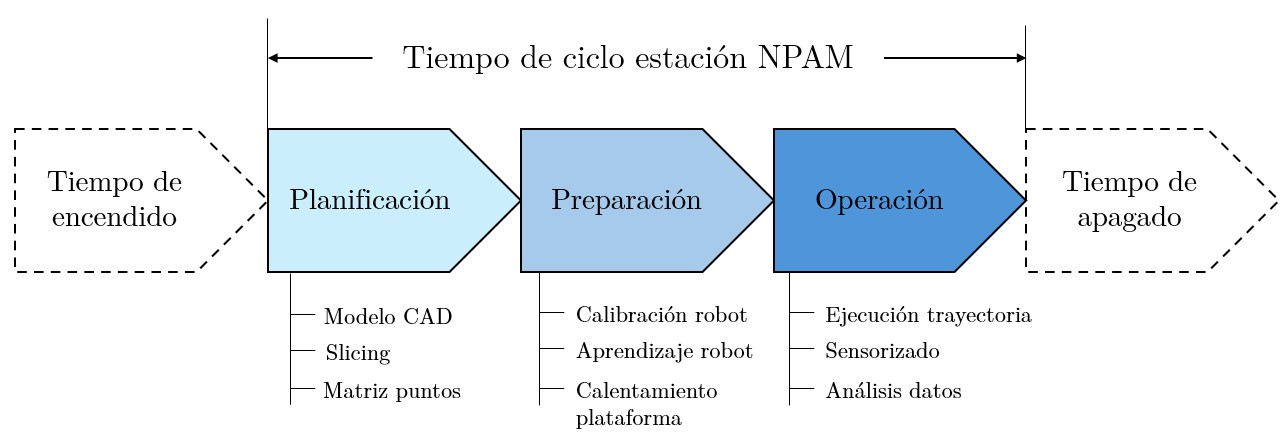
\includegraphics[scale=0.45]{figuras/tiempo_ciclo_estacion_v2.jpg}
    \caption{Flujo de trabajo expresado como tiempo de ciclo}
    \label{fig:tiempo_ciclo_estacion}
\end{figure}

Durante el tiempo de \textit{Planificación} se llevarán a cabo las tareas de diseño \acrshort{CAD} de la pieza a fabricar para que pase por un proceso de slicing. El resultado del slicer será un conjunto de puntos ordenados en el espacio en forma de matriz que representará cada ubicación exacta de deposición de material.

El tiempo de la fase de \textit{Preparación} se empleará en establecer, de forma previa a la ejecución del proceso de fabricación. los principales parámetros de control de la estación. Las operaciones clave de esta etapa se efectuarán en el siguiente orden: 
    \begin{enumerate}
        \item \textbf{Calibración del robot:} Para definir las relaciones entre los diferentes sistemas de referencia de la estación y la matriz de puntos obtenida de la etapa de \textit{Planificación}.
        \item \textbf{Aprendizaje del robot:} Para elaborar un conjunto de trayectorias y poses robotizadas a ejecutar. Dichas poses estarán enfocadas no solo en la deposición de material en los puntos indicados por la etapa de planificación, si no también en la gestión de riesgos de colisiones con otros elementos.
        \item \textbf{Calentamiento previo de la plataforma:} Comienza una vez que se haya validado que la trayectoria calculada es segura. Este proceso emitirá una señal de arranque de la operación en cuanto que se haya validado que la temperatura de la plataforma de impresión es la deseada y se mantiene estable.
    \end{enumerate}

El último tiempo es el de la etapa de \textit{Operación}, la cual comenzará una vez que se haya verificado la consecución completa de todas las tareas que conforman la \textit{Preparación}. En el transcurso de esta fase, el manipulador robótico efectuará la trayectoria calculada a través de los modelos de aprendizaje y se solicitará a una unidad de cómputo central el muestreo de datos de interés (posiciones, temperaturas, inercias del sistema, ...) Dichos datos podrán ser analizados en momentos posteriores con el objetivo de aportar mejoras sobre el proceso de fabricación y valorar su rendimiento.

\subsubsection*{Arquitectura}
\hypertarget{Arquitectura}{}
\bookmark[level=subsubsection,dest=Arquitectura]{Arquitectura}
La labor de diseño de la arquitectura informática se plantea teniendo en cuenta algunos de los aspectos planteados en la sección \ref{sec: arquitecturas_informaticas_estado_arte}, en la que se observó cómo aquellas soluciones que integran controladores especializados en diferentes tareas y niveles de abstracción han sido las de mayor éxito. Algunos de estos elementos especializados pueden ser la existencia de un controlador central, la disposición de una interfaz entre máquina y humano, el uso de varias capas de comunicaciones especializadas o un controlador exclusivo para el robot.

La Figura \ref{fig:arquitectura_TFM} muestra el diseño de arquitectura final realizado. Este diseño también sirve para definir el flujo de trabajo de la estación describiendo cinco grupos funcionales:
\begin{enumerate}
    \item \textbf{Slicer:} Elemento responsable de generar la trayectoria cartesiana de \textit{slicing} a partir del modelo \acrshort{CAD} de la pieza. Señalado en color rosa.
    \item \textbf{Computador central:} Señalado en color rojo, es el sistema informático que sirve de nexo entre el resto de elementos de la estación. Es el responsable de:
    \begin{itemize}
        \item Calcular los movimientos del robot a partir de las trayectorias del proceso de slicing.
        \item Operar el entorno de trabajo virtual del robot.
        \item Gestionar los mensajes del resto de grupos funcionales.
        \item Revisión de estado del resto de elementos.
    \end{itemize}
    \item \textbf{Plataforma de impresión:} Grupo funcional correspondiente a la gestión de la cama de impresión en cuanto a su control de temperatura y comunicaciones con el computador central. La gestión de estas tareas caen a cargo de una unidad de control que hace de interfaz entre el sistema de calentamiento de la cama y el resto de la estación. Todos sus componentes están coloreados en naranja.
    \item \textbf{Robot  UR:} Robot colaborativo responsable de recibir las trayectorias calculadas por el computador central. Este grupo funcional integra otras funcionalidades como aportar la calibración del robot y la toma provenientes de diferentes sensores conectados a su \acrshort{PLC}. Todos los equipos hardware y software que lo componen se identifican con el color amarillo.
    \item \textbf{Extrusor:} Sistema de control del extrusor de material de la estación. De forma análoga a la cama de impresión debe ser capaz de controlar automáticamente variables internas como son el flujo de material extruído, su temperatura o la corriente eléctrica demandada. Este grupo se identifica con el color verde claro.
\end{enumerate}

\begin{figure}[h!]
    \centering
    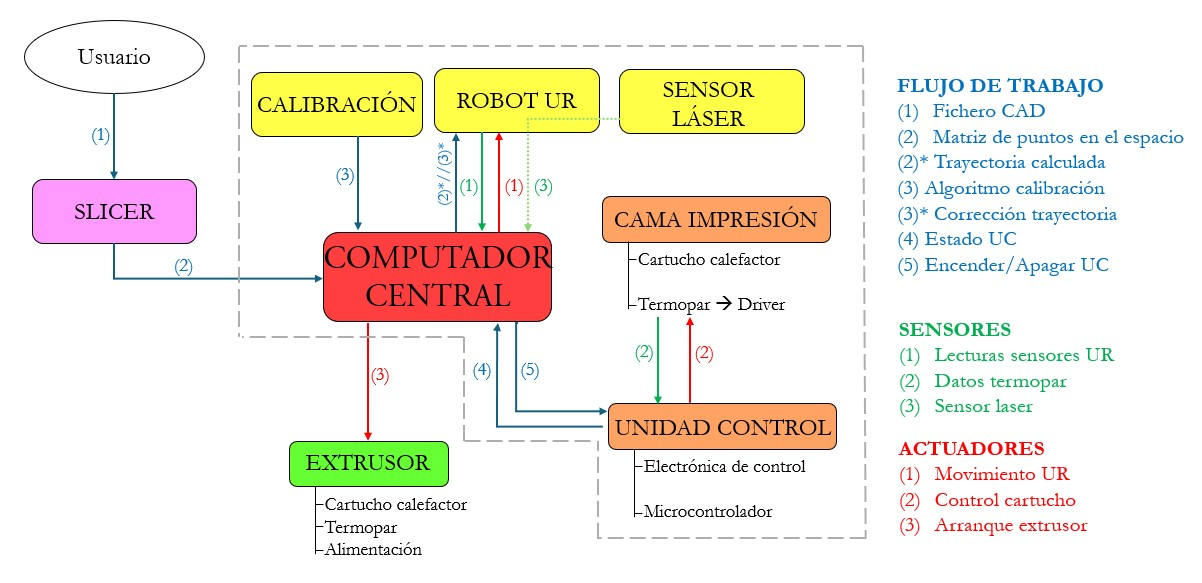
\includegraphics[scale=0.55]{figuras/arquitectura_TFM_v3.jpg}
    \caption{Arquitectura planteada en este proyecto}
    \label{fig:arquitectura_TFM}
\end{figure}

Por motivos de alcance del trabajo se toma que aquellos grupos funcionales en los que se trabajará son los encuadrados dentro de una línea de rayas gris en la Figura \ref{fig:arquitectura_TFM}. Es decir, en este proyecto sólo se tratarán los grupos funcionales del \textit{Computador central}, la \textit{Plataforma de impresión} y el \textit{Robot UR}. Los grupos funcionales de \textit{Slicer} y \textit{Extrusor} quedan a cargo de otros integrantes del marco de proyecto. 

Algunos elementos de los grupos funcionales describen otros componentes a un nivel de abstracción inferior. Por ejemplo es el grupo funcional del extrusor, que de forma análoga cuenta con un cartucho calefactor para el aporte de calor al sistema y un termopar como sensor de temperatura. Sin embargo, también efectúa otras funciones como la regulación del caudal de material de alimentación. Otro ejemplo, es el caso de la plataforma de impresión. Este grupo establece en la unidad de control un elemento regulador relé conectado a un microcontrolador que ha sido programado para regular su apertura a través de código. Por otra parte, la cama de impresión cuenta con un cartucho calefactor y un termopar que actúa como sensor de temperatura conectado al microcontrolador gracias a su propio driver..

Para la comunicación entre grupos funcionales se han definido mensajes especializados según el tipo de información que transcriben y la tarea dentro de la que se enmarcan. Los mensajes pueden referirse a información relacionada con el flujo de trabajo de la estación, la información de los sensores y las señales de activación de los actuadores.

Entre los mensajes relacionados con el flujo de trabajo de la estación (marcados en color azul en la Figura \ref{fig:arquitectura_TFM}) se encuentran:
\begin{itemize}
    \item \textbf{Fichero \acrshort{CAD}:} Modelo 3D diseñado por el usuario. Este modelo en formato \acrshort{STL} pasa a través del slicer para obtener el conjunto de puntos en el espacio donde se depositará el material extruído. 
    \item \textbf{Matriz de puntos en el espacio:} Es el resultado del slicing del modelo \acrshort{CAD} en forma de matriz. Estos puntos se sitúan sobre la plataforma de impresión y se referencian a un origen de coordenadas globales ubicado en la base del robot UR. Cada fila de la matriz representa a un único punto con posición cartesiana y orientación en forma de cuaternión unitario. Las tres primeras coordenadas del punto es la posición \textit{xyz} del punto, mientras que las cuatro últimas son las coordenadas \textit{ijkw} del cuaternión que indica la orientación. La Ecuación \ref{eq: punto_slicer} muestra un ejemplo de esta representación para el i-ésimo punto de la matriz.

    \begin{equation}
        \boldsymbol{p_i}= \begin{bmatrix}
            x_i & y_i & z_i & | & i_i& j_i& k_i& w_i 
        \end{bmatrix}
        \label{eq: punto_slicer}
    \end{equation}

    \item \textbf{Trayectoria  calculada:} La matriz de puntos elaborada en el proceso de slicing pasa al computador central, quien se responsabiliza de efectuar una lectura sobre ella y utilizar el controlador de ROS2 implementado para calcular su cinemática inversa. Esto es, se obtiene el conjunto de posiciones que debe adoptar el robot para alcanzar dichos puntos del espacio. Este mensaje se transmite al \acrshort{PLC} del robot para que su controlador integrado pueda aplicar dichos desplazamientos, se indica con el símbolo $(2)*$ para indicar que resulta del procesamiento directo de a través de ROS2 de la matriz de puntos. La definición explícita de este mensaje se indica en el capítulo \ref{cap: trayectorias}.

    \item \textbf{Algoritmo de calibración:} Es la parametrización de la calibración intrínseca del robot UR. Se define en formato \acrshort{YAML} indicando cómo se enlaza cada eslabón del robot con el siguiente y sus posiciones en el espacio. También se indican parámetros de interés como pueden ser los centros de inercia o el peso de cada eslabón. Este mensaje se inserta como un dato anexo que debe tener en cuenta la implementación ROS2 del computador central cuando se calcule la trayectoria articular.

    \item \textbf{Corrección de la trayectoria:} Trayectoria corregida gracias al controlador empleado dentro del controlador de ROS2 para tener en cuenta la calibración intrínseca del manipulador robótico y sus inercias, así como también los esfuerzos requeridos en cada articulación. Este mensaje se procesa en la implementación ROS2 del computador central de forma paralela a la trayectoria calculada, implementándose a modo de acción correctora sobre la misma. Esta relación entre ambos mensajes se indica con el símbolo $//$ para indicar un procesamiento paralelizado en el tiempo y $(3)*$ para resaltar que proviene de un procesamiento directo por parte de la implementación ROS2.

    \item \textbf{Estado de la Unidad de Control (UC):} Consigna de estado objetivo que debe alcanzar la unidad de control de temperatura de la cama de impresión. Este mensaje se manda directamente desde el computador central y es unidireccional, la responsabilidad de su correcto procesamiento recaerá sobre la unidad de control de la plataforma de impresión.

    \item \textbf{Encedido/Apagado de Unidad de Control (UC):} Mensaje de estado proporcionado por la propia unidad de control para indicar su activación y posibilidad de ejecución de trayectoria, así como un caso de apagado de emergencia.
\end{itemize}

Los mensajes relacionados con las señales de los sensores se indican en color verde en la Figura \ref{fig:arquitectura_TFM}, entre ellos destacan:
\begin{itemize}
    \item \textbf{Lectura de los sensores del manipulador UR:} Se sirven de la implementación ROS2 del computador central para proporcionar información constante de la configuración cinemática del robot (posiciones, velocidades y esfuerzos articulares). Estos datos se toman directamente desde el controlador \acrshort{PLC}, que hace de interfaz con los sensores internos del UR.

    \item \textbf{Datos del termopar:} Lectura de temperatura alcanzada en la cama de impresión. Esta información se procesa con un driver de lectura de dicho sensor y a continuación es integrada en el mensaje de Estado de la UC que se manda al computador central.

    \item \textbf{Sensor láser:} Medida de intensidad proporcionada por el sensor láser de la estación. Dicho sensor se conecta al \acrshort{PLC} del manipulador, por lo que se necesita implementar un sistema de lectura de entradas analógicas de dicho controlador con ROS2. Esta necesidad se ve representado con la línea de puntos verde que atraviesa el bloque de \textit{Robot UR} de la Figura \ref{fig:arquitectura_TFM}.
\end{itemize}

El color rojo corresponde a los mensajes de los actuadores que participan en la aquitectura informática de la Figura \ref{fig:arquitectura_TFM}. Estos mensajes son órdenes explícitas e inalterables que provienen del procesamiento de un controlador existente aguas arriba. Los más destacados son:
\begin{itemize}
    \item \textbf{Movimiento UR:} Orden de ejecución de movimiento del robot tomando como referencia la trayectoria calculada en el flujo de trabajo. Está comandada directamente desde el computador central.
    \item \textbf{Control del cartucho calefactor:} Mensaje que habilita la circulación de corriente a través del cartucho calefactor integrado dentro de la cama de impresión para aumentar su temperatura hasta el valor deseado. Buscando una mayor modularidad de la arquitectura, se decide que sea un mensaje gestionado únicamente desde la UC.
    \item \textbf{Arranque del extrusor:} Señal de arranque del mecanismo extrusor de material. Proviene desde el computador central y su definición queda fuera del alcance de este proyecto.
\end{itemize}


\section{Resultados y conclusiones}
Como resultado de la metodología implementada se expone un ejemplo de control general de la estación. En este caso se opta por la ejecución de una trayectoria robótica mientras se registran datos de las configuraciones cinemáticas adoptadas por el manipulador robótico haciendo uso del \acrshort{PLC} integrado y las posibilidades que ofrece ROS2 en este tipo de entornos. 

Dada la naturaleza mayor nivel de abstracción de este capítulo, este proceso se presenta como un ejemplo de los resultados obtenidos gracias a la metodología de diseño seguida. En posteriores capítulos se procederá a explicar de forma más concreta los fundamentos técnicos de cada una de las secciones de la arquitectura propuesta.

\subsection{Ejemplo de implementación}
\label{sec: ejemplo implementacion diseño arquitectura}

Se procede al cálculo y ejecución de una trayectoria sencilla para validar el correcto funcionamiento de las distintas unidades de la arquitectura y las comunicaciones que utilizan entre sí. El movimiento que debe seguir el \acrshort{TCP} del manipulador robótico se muestra en la Figura \ref{fig:trayectoria_objetivo}. Este movimiento cumple con las características definidas en trabajos de referencia para este proyecto \cite{paper_Q1_Alvaro_Adrian}\cite{TFM_SanchoAmparo}, y es el que se ha usado en los ensayos especializados para la validación de ejecución de trayectorias complejas y la calidad de la calibración introducida en el entorno de trabajo ROS2.  

Se trata de medio muelle de perfil cilíndrico que se fabrica depositando material sobre la cama de impresión. En capítulos posteriores se analizará con más detalle el desempeño del manipulador robótico junto al sistema de cálculo y ejecución cinemática, así como también la gestión de diferentes mensajes y la posibilidad de futuros análisis de datos.

\begin{figure}[h!]
    \centering
    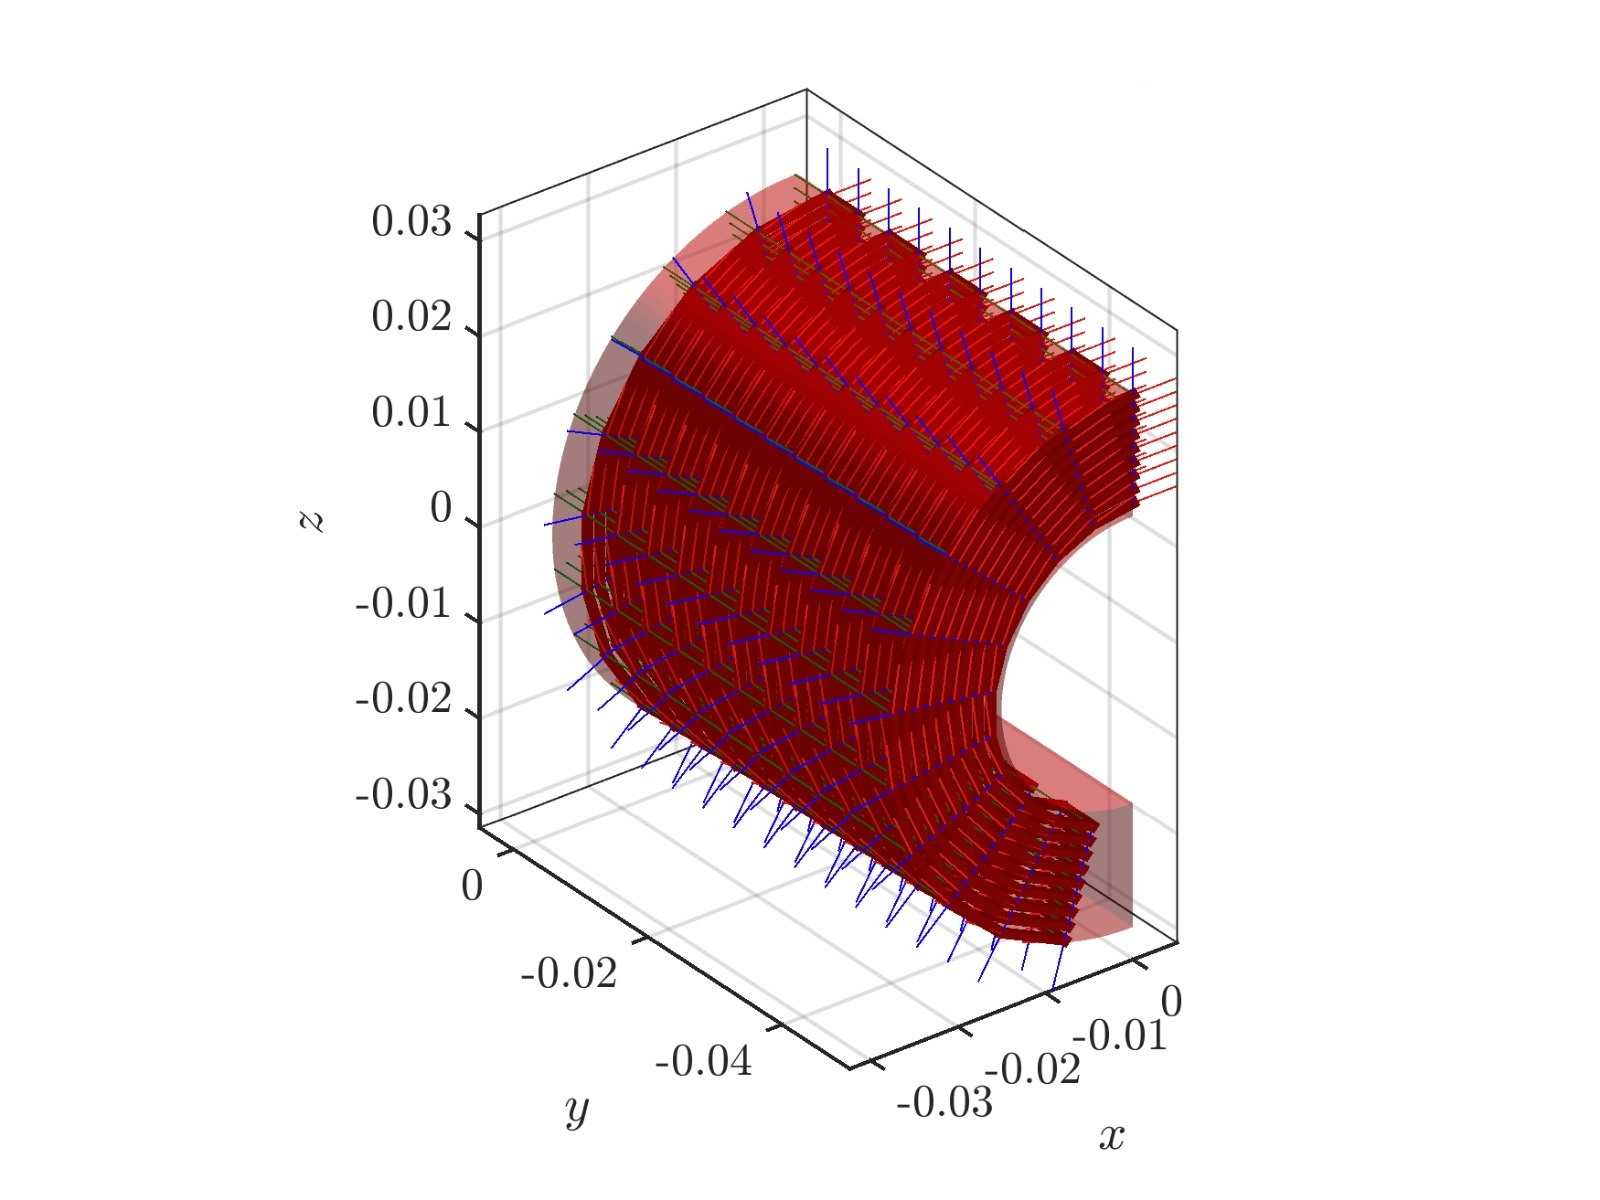
\includegraphics[scale=0.3]{figuras/trayectoria_objetivo.jpg}
    \caption{Trayectoria objetivo del ejemplo}
    \label{fig:trayectoria_objetivo}
\end{figure}

Se comienza arrancando el computador central e invocando una instancia del sistema de planificación offline. Este sistema se fundamenta en el empleo del controlador de ROS2 Moveit para las tareas de:

\begin{enumerate}
    \item Definición del espacio de trabajo.
    \item Imposición de restricciones de cálculo de trayectorias.
    \item Lectura de ficheros CSV de trayectoria objetivo resultado del proceso de slicing.
\end{enumerate}

Con estas tareas en mente se añade para este ejemplo una más: el muestreo de datos en directo relacionados con el desempeño del manipulador robótico durante la trayectoria efectuada.  

Con el entorno de trabajo virtualizado definido se abre una terminal que pueda establecer una comunicación directa con el manipulador. En el caso de este trabajo se opta por implementar un sistema basado en ROS2 que implemente el controlador cinemático Moveit. En otra terminal en paralelo, se accede invocar el nodo de ROS2 que llevará el grueso de la tarea. 

El procedimiento consiste en la invocación de un nodo perteneciente a un paquete de mayor nivel de abstracción conocido como \textit{rutine\_launcher}. El paquete \textit{rutine\_launcher}\footnote{Disponible en el repositorio del trabajo en la dirección:  \textit{./workspace/ros\_ur\_driver/src/rutine\_launcher/rutine\_launcher}} está enfocado en la definición y gestión de rutinas, es decir, la ejecución de nodos especializados en diversas tareas que trabajan bajo una estructura común. 

El nodo de este ejemplo combina el cálculo cinemático del manipulador, con el muestreo en directo de datos desde el \acrshort{PLC}. Este nodo se llama \textit{super\_logger\_launcher} y su funcionamiento se basa en la ejecución de instrucciones de ROS2 modulares, es decir, en la invocación síncrona de dos nodos. Un acercamiento a su forma de trabajar se aprecia en el pseudocódigo \ref{alg:algoritmo_super_logger_launcher}.


\begin{algorithm}[h!]
\caption{super\_logger\_launcher}\label{alg:algoritmo_super_logger_launcher}
\begin{algorithmic}[1]
\Require Entradas respectivas de los paquetes ROS2 especializados
\Ensure Ejecución de trayectoria simultánea al muestreo de datos UR
\State Definir la instrucción de invocación del nodo de cálculo y ejecución de cinemática
\State Definir la instrucción de invocación del nodo de muestreo de señales del PLC
\State Invocar una instancia del nodo de ejecución de trayectorias
\State Invocar una instancia del nodo de muestreo de señales PLC
\State Crear un suscriptor para el nodo de ejecución de trayectorias
\State Suscribir el nodo de muestreo de señales al suscriptor de las trayectorias

\If{Suscripción correcta}
    \State Cálculo de trayectoria
    \State Envío de señal de fin de cálculo de trayectoria a nodo de muestreo
    \If{Fin de cálculo de trayectoria == True}
        \State Ejecutar trayectoria
        \State Comenzar muestreo de datos
    \Else 
        \State Ejecutar trayectoria
        \State Mostrar error de muestreo
    \EndIf
\EndIf

\end{algorithmic}
\end{algorithm}

El algoritmo implementado se aprovecha de algunas características de los sistemas ROS como son la paralelización de procesos o el uso de comunicaciones síncronas entre los procesos del computador central. Para disminuir el grado de error se modifica la velocidad preestablecida en el entorno virtual para que se deje un pequeño margen de tiempo entre la señal de ejecución de trayectoria, el arranque del muestreado de datos y el comienzo del propio movimiento del robot. Esta velocidad se ha ajustado de forma estocástica ya que depende en gran medida del funcionamiento de la unidad integrada en la arquitectura.

\subsection{Resultados}
El robot es capaz de ejecutar la trayectoria encomendada por el nodo especialista en el cálculo de trayectorias de forma eficaz. Del mismo modo, es posible tomar un muestreo de las configuraciones cinemáticas de cada articulación del manipulador en tiempo real para posteriormente compararlas con las calculadas por el controlador ROS2 integrado en el sistema.

La Figura \ref{fig:ejemplo_muestreo} muestra el valor de cada posición articular calculada para la trayectoria  ensayada. Nótese cómo al tratarse de un movimiento rotativo de una articulación (la número 4 en este caso) mientras el resto permanecen prácticamente fijas, se observa que la articulación de giro sobre la que se apoya la plataforma de impresión muestra un trazado similar al de una señal sinusoidal. 

Por otro lado, el resto de articulaciones son las responsables de avanzar en el eje longitudinal de la cama y de variar en pequeños escalones la cota de impresión. Es decir mantienen un valor prácticamente constante en todo el tiempo de ejecución que solamente sufre correcciones periódicas en el momento de variar la altura de capa

\begin{figure}[h!]
    \centering
    \includegraphics[scale=0.30]{figuras/ejemplo_muestreo.png}
    \caption{Posiciones articulares registradas durante el movimiento automático}
    \label{fig:ejemplo_muestreo}
\end{figure}

\subsection{Conclusiones}
Como se ha observado en el ejemplo de implementación, el sistema tiene capacidad para gestionar tareas complejas con relativa facilidad. Es decir, el computador central puede adaptar el tipo de mensaje que necesita cada unidad especializada para que sea ejecutado con precisión y teniendo en cuenta el entorno de trabajo real en el que se mueve el manipulador robótico.

La presencia de módulos especializados favorece la inserción de nuevos dispositivos al sistema, como puede ser en este caso el sensor láser o la lectura directa del \acrshort{PLC}. Tanto la lectura de datos como la ejecución de trayectorias se hacen utilizando como base la interfaz de programación dispuesta por ROS2. Es decir, se facilita la labor de validación de trayectorias siguiendo fundamentalmente la filosofía del aprendizaje offline.
No obstante. la capacidad de toma de datos directa del manipulador también favorece introducir una parte de aprendizaje online, dejando siempre libre la posibilidad de registrar un movimiento del cobot guiado por el operario a partir del cual generar una nueva trayectoria. 

De igual modo, la interfaz introducida en el paquete de lanzamiento de rutinas, facilita la definición de paquetes más sencillos con los parámetros deseados por el operario, dejando un control total sobre aspectos que se describirán con más detalle en los siguientes capítulos como pueden ser el número de muestras, la temperatura de calentamiento de la cama o la velocidad de ejecución del movimiento. Esto es, se realiza una gestión de las comunicaciones entre diferentes unidades funcionales utilizando los conceptos aportados por el entorno de trabajo ROS2, cuyo grafo de conexionado completo se puede consular en el anexo \ref{cap: anexo grafos nodos ros2}.
\chapter{Sistema de lectura de datos del robot}
\label{cap:lectura_datos}

Este capítulo entra en detalles técnicos de una de las tres funcionalidades principales de la estación diseñada: el sistema de muestreo y lectura de datos. Se comenzará haciendo una breve introducción al problema, comentando las variables de interés que se desean registrar y el funcionamiento deseado para el sistema. 

A continuación, se describirá el procedimiento que se ha empleado para utilizar ROS2 como cimiento de las señales registradas por el computador central de la estación. En la siguiente sección se presentará un caso de uso en el que se mostrará como resultado el registro de las variables seleccionadas anteriormente. Como punto final al capítulo, se comentarán las principales ventajas del sistema implementado, así como posibles mejoras por añadir en un futuro.

El código descrito en este capítulo se encuentra disponible en el repositorio GitHub del proyecto \cite{repo_github_TFM_MiguelLerinAlonso}. Los nodos de ROS2 que representan dichas tareas pertenecen al paquete \textit{data\_logger}\footnote{Disponible en el direccionamiento: \textit{./workspace/ros\_ur\_driver/src/data\_logger}}.

\section{Introducción al problema}
Actualmente las estaciones de fabricación deben registrar de forma continuada variables de importancia para el proceso que llevan a cabo. En el caso de las estaciones \acrshort{MEX}, estas variables suelen estar relacionadas con parámetros como pueden ser la posición del extrusor, la temperatura del material depositado o la altura de capa conseguida en cada nueva iteración.

El paradigma propuesto por los procesos \acrshort{NPAM} introduce ciertas modificaciones a las variables antes mencionadas. Dichas modificaciones cobran más relevancia especialmente si se trabaja con una plataforma de impresión móvil acoplada a un manipulador robótico, como puede ser el caso del presente proyecto.

De acuerdo con la arquitectura de control definida en el capítulo \ref{cap: diseno_arquitectura}, los datos provenientes de los sensores partícipes están involucrados con (1) la configuración cinemática adoptada por el robot en cada instante, (2) la información proveniente de la plataforma de impresión y (3) la lectura aportada por un sensor láser de distancia. Estas tres familias de datos de importancia deben procesarse por parte del computador central, que en última instancia será el responsable de su adecuada gestión.

Se busca la definición de una interfaz software que pueda gestionar aguas abajo del computador central toda esta información. La interfaz debe ser lo suficientemente flexible para permitir una lectura rápida de la información interna de la estación sin interferir en el proceso de fabricación que se esté llevando a cabo. En otras palabras, ha de integrarse con el movimiento del manipulador robótico y el control de temperatura de la cama de impresión.

\section{Metodología}
La construcción del sistema de lectura de datos presente en este proyecto atraviesa dos etapas diferenciadas. En la primera se seleccionan las variables de interés a las que debe poder acceder el sistema, al mismo tiempo se define el modelo de arquitectura de nodos ROS2 que se seguirá. La segunda etapa describe el proceso de creación de dicho sistema, haciendo especial en la escalada desde las unidades de código más atómicas hasta las de mayor nivel de abstracción.

\subsection{Selección de variables de interés}
Se procede al estudio de las capacidades de cada uno de los equipos hardware que participan en la estación robotizada, siendo aquellos que quedan dentro del alcance del proyecto el manipulador robótico UR, el sensor de distancia láser y la plataforma de impresión. Las variables de control de cada equipo, es decir, aquellas que pueden ofrecer información relevante sobre su estado son:

\begin{itemize}
    \item \textbf{Manipulador robótico:} Es el equipo responsable del movimiento de la plataforma de impresión según la trayectoria introducida y la velocidad comandada por el operario. Sus variables de interés serán aquellas que permitan definir de forma rápida su configuración cinemática en el espacio, como son la posición y velocidad de giro de cada articulación. Otras variables relacionadas con su comportamiento dinámico -como el caso de los esfuerzos articulares- también se consideran de interés de cara a futuros proyectos.
    \item \textbf{Sensor de distancia láser:} Este equipo permite validar la trayectoria efectuada por el manipulador robótico, midiendo la distancia existente entre el foco de energía láser y el punto de incidencia con la plataforma de impresión. Su variable de interés será dicha distancia.
    \item \textbf{Plataforma de impresión:} Su tarea principal es alcanzar y regular la temperatura comandada por el computador central. Es decir, la variable de interés es la temperatura registrada por el termopar en cada instante. Este dispositivo constituye uno de los componentes más modulares de la estación, por lo que se opta por dotarle de su propio sistema de comunicación con el computador central. La metodología seguida para dicha tarea se describe en el capítulo \ref{cap: control_temperatura}.
\end{itemize}

Se debe tener en cuenta que la frecuencia de actualización de cada variable puede depender directamente del equipo utilizado, por lo que será necesario emplear siempre una frecuencia de muestreo al menos dos veces superior a la de actualización del fenómeno registrado. En este caso, las principales limitaciones serán las aportadas por el \acrshort{PLC} integrado en el robot UR y la frecuencia de actualización impuesta en la unidad de control de la cama de impresión. Se considera que el procesador del computador central puede trabajar a una frecuencia más que suficiente para no ser una limitación.

Aprovechando la instalación existente en el laboratorio, se aprovecha la comunicación por MODBUS \acrshort{TCP/IP} para conectar directamente el computador central a la mesa de trabajo del manipulador robótico a utilizando un cable Ethernet. Este enfoque queda definido de cara a la interacción con otros equipos -como es el caso del sensor de distancia láser- que deben conectarse al \acrshort{PLC} del robot. El motivo principal por el que se selecciona esta solución es la necesidad de establecer un sistema de comunicaciones sencillo y confiable con un protocolo de comunicación industrial sobre el cuál ya habían trabajos previos para realizar sucesivas validaciones. 

Esto es, siguiendo la filosofía descrita por el capítulo \ref{cap: diseno_arquitectura} se busca que los componentes de la estación de fabricación puedan comunicarse entre sí sin necesidad de depender de elementos externos, como puede ser una conexión inalámbrica.

\subsection{Definición del sistema}
Con las variables de interés definidas se procede a evaluar el tipo de señal adecuado para cada una. Se tienen como factores de interés no solamente el equipo responsable de cada una, si no también su integración con diferentes protocolos de comunicación y equipos disponibles. En los siguiente párrafos se exponen el sistema de comunicaciones implementado para cada equipo, así como las razones detrás de la elección de una alternativa frente a otras.

\subsubsection*{Manipulador robótico}
\hypertarget{Manipulador robótico}{}
\bookmark[level=subsubsection,dest=Manipulador robótico]{Manipulador robótico}
Las configuraciones cinemáticas del manipulador robótico, así como la medida de sus esfuerzos articulares, son variables internas del equipo; motivo por el que su acceso no es inmediato y se debe disponer de una capa de software especializado en su registro y control. Con dicha limitación establecida, se opta por utilizar el entorno proporcionado por ROS2 Humble y en concreto, el controlador de UR para entornos de programación ROS2 \cite{UniversalRobots_ROS2_Driver}.

El controlador de UR basa su funcionamiento en una capa de software intermedia entre la versión de ROS2 empleada y el controlador Moveit, de modo que permite adaptar nodos de ambos sistemas a una versión específica para los equipos de la compañía. Dicha versión es capaz de gestionar automáticamente aspectos fundamentales de la definición del cobot como pueden ser sus ficheros de calibración, los controladores de movimiento o la lectura optimizada de variables internas. Esto resulta de gran utilidad no solamente para acceder de forma cómoda a valores articulares si no también a los diferentes registros de su \acrshort{PLC} integrado.

Puesto que la intención del sistema de registro de datos es elaborar un conjunto de solicitudes periódicas al robot UR que se vayan efectuando durante el tiempo de medida, se opta por emplear una arquitectura de ROS2 basada en el modelo publicador-suscriptor. En el modelo implementado en esta sección, el publicador será el robot, que deberá responder a la solicitud continuada del computador central proporcionando información en tiempo real. 

La información del manipulador, al estar directamente relacionada con los valores de posición, velocidad y esfuerzo articulares en cada instante de medida, debe responder a un nodo del entorno ROS2 especializado en dicho registro llamado \textit{joint\_states}. Siguiendo la terminología de ROS2, este nodo asume la tarea de publicador mientras que el paquete de lectura de datos -en concreto aquel nodo especializado en valores articulares- asumirá el papel de suscriptor. El nodo suscriptor se llama \textit{joint\_reader} y su funcionamiento queda descrito en el algoritmo \ref{alg:algoritmo_joint_reader}. 

\begin{algorithm}[H]
\caption{joint\_reader}\label{alg:algoritmo_joint_reader}
\begin{algorithmic}[1]
\Require Muestras totales que se desean realizar
\Ensure Vector de configuraciones articulares en tabla CSV

\State Arrancar el nodo como suscriptor de \textit{joint\_states}
\State Configurar la función de callback con el número de muestras deseadas

\While{Número de muestra $<$ Muestras totales}
    \State Leer configuraciones articulares de \textit{joint\_states}
    \State Almacenar valor leído en vector resultado
\EndWhile

\State Guardar vector resultado en tabla CSV

\end{algorithmic}
\end{algorithm}

El algoritmo \ref{alg:algoritmo_joint_reader} se presenta como una versión generalizada del procedimiento descrito, por lo que es fácilmente escalable a variables como posiciones, velocidades y esfuerzos articulares. El parámetro de entra principal es el número de muestras que se desean tomar, aunque también se definen otros valores como la ruta de guardado dentro del sistema de ficheros del computador central.

La Figura \ref{fig:nodo joint_reader rqt_graph} muestra en forma de grafo el conexionado del nodo \textit{joint\_reader} dentro del espacio de nodos que proporciona ROS2. Nótese cómo dicho nodo se suscribe únicamente el mensaje proveniente de \textit{joint\_states} y lo publica como una salida del sistema a través del mensaje genérico \textit{rosout}. De acuerdo con el firmware proporcionado por ROS2, en la parte superior de la imagen se muestra cómo interpreta a cada nodo y mensaje de forma automática. Siendo la publicación de \textit{joint\_states} un nodo de arquitectura publicador o \textit{publisher}, \textit{joint\_reader} el intermediario que hace las transformaciones necesarias entre el tipo de mensaje que se le proporciona y \textit{rosout} el escucha final ubicado aguas abajo al final de toda la información gestionada.

\begin{figure}[h!]
    \centering
    \includegraphics[scale=0.15]{figuras/nodo joint_reader rqt_graph.png}
    \caption{Grafo de estructuración del nodo \textit{joint\_reader}}
    \label{fig:nodo joint_reader rqt_graph}
\end{figure}


\subsubsection*{Sensor de distancia láser}
\hypertarget{Sensor de distancia láser}{}
\bookmark[level=subsubsection,dest=Sensor de distancia láser]{Sensor de distancia láser}

El sensor de distancia se caracteriza por enviar una señal analógica de corriente proporcional a la lectura. Al tratarse de un valor analógico que debe estar en constante comunicación con el manipulador robótico, se opta por conectarlo al \acrshort{PLC} a través de una de sus entradas digitales por mayor sencillez. La recta de calibración se muestra en la ecuación \ref{eq: calibracion sensor laser}.

\begin{equation}
\label{eq: calibracion sensor laser}
    d [m]=(0.035-0.025) \frac{I[A]-0.004}{0.02-0.004}+0.025 
\end{equation}

Es decir, se plantea un lector especializado en las entradas y salidas del \acrshort{PLC}. Este lector se sirve de la interfaz software proporcionada por el controlador de UR para ROS2, en concreto se accede al nodo \textit{/io\_and\_status\_controller/io\_states}. Este nodo proporciona una interfaz accesible tanto para entradas como para salidas, independientemente de si su naturaleza es digital o analógica. 

Por este motivo se plantea el algoritmo \ref{alg:algoritmo_analog_reader} como una referencia de funcionamiento tanto para señales digitales y analógicas. Los nodos de ROS2 responsable del muestreo de dichas señales se llaman respectivamente digital\_reader y analog\_reader. Ambos nodos reutilizan la estructura de publicador-suscriptor empleada en el lector de configuraciones articulares.

\begin{algorithm}[h!]
\caption{analog\_reader}\label{alg:algoritmo_analog_reader}
\begin{algorithmic}[1]
\Require Muestras totales que se desean realizar
\Ensure Vector de lecturas analógica

\State Arrancar el nodo como suscriptor de \textit{/io\_and\_status\_controller/io\_states}
\State Configurar la función de callback con el número de muestras deseadas

\While{Número de muestra $<$ Muestras totales}
    \State Leer valor de la señal muestreada
    \State Almacenar valor leído en vector resultado
\EndWhile

\State Guardar vector resultado en tabla CSV
\end{algorithmic}
\end{algorithm}

La Figura \ref{fig:nodo analog_reader rqt_graph} vuelve a utilizar el enfoque antes mencionado y muestra el grafo de conexionado entre los nodos responsables de lectura de puertos del \acrshort{PLC} y los nodos propios de ROS2 que proporcionan dicha información. 

\begin{figure}[h!]
    \centering
    \includegraphics[scale=0.15]{figuras/nodo analog_reader rqt_graph.png}
    \caption{Grafo de estructuración del nodo \textit{analog\_reader}}
    \label{fig:nodo analog_reader rqt_graph}
\end{figure}

Cabe destacar que en este tipo de nodos se introducen nuevas configuraciones referentes a la frecuencia de muestreo, la definición del pin o si se trata de un valor de entrada o salida al \acrshort{PLC}. La definición de estos parámetros se explica con mayor detalle en el repositorio Git del proyecto\cite{repo_github_TFM_MiguelLerinAlonso}, en cuanto a la tarea de explicar el funcionamiento del sistema, no obstante dicha información se encuentra descrita y comentada en el repositorio del proyecto \cite{repo_github_TFM_MiguelLerinAlonso}.

\subsubsection*{Lectura del robot}
\hypertarget{Lectura del robot}{}
\bookmark[level=subsubsection,dest=Lectura del robot]{Lectura del robot}

Teniendo ya implementada una versión básica de lectores para cada tipo de datos provenientes de todos aquellos equipos de la estación relacionados directamente con el manipulador robótico, se procede a integrar dichos nodos de ROS2 en un esquema superior haciendo uso del soporte para \acrshort{POO}. Esto es, se define cada uno de los nodos antes descritos como una clase hija de una de mayor nivel de abstracción que pueda gestionar ambas al mismo tiempo. 

Esta nueva clase se conoce por el nombre de \textit{super\_logger} y se caracteriza por su capacidad de iniciar un registro en un proceso paralelo a la ejecución de trayectorias por parte del robot. La facilidad del nodo para realizar dicha tarea se debe a que integra dos nodos hijos que siguen el esquema de publicador-suscriptor, por lo que el propio nodo padre sigue dicho esquema. Dicho registro se puede definir a través de parámetros de interés como son el número de muestras deseadas, la frecuencia de muestreo, los pines del \acrshort{PLC} que se desean leer o el tipo de señal entre otros. 

El resultado de la lectura se guarda de forma predeterminada en una tabla CSV de forma automática\footnote{Disponible en el direccionamiento: \textit{./workspace/ros\_ur\_driver/src/data\_logger/results}}, aunque existe la posibilidad de indicar al sistema que continúe con el registro de datos por terminal una vez que haya guardado la tabla CSV. Los campos disponibles en dicha tabla son:

\begin{itemize}
    \item Número de muestra del registro
    \item Marca de tiempo en formato Unix
    \item Vector de posiciones articulares
    \item Vector de velocidades articulares
    \item Vector de esfuerzos articulares
    \item Estado de salida/entrada analógica
    \item Estado de salida/entrada digital
\end{itemize}

Cabe destacar que los vectores de configuraciones articulares constan de un total de 6 coordenadas, cada una correspondiente a una articulación del modelo definido en el entorno ROS2. Por comodidad en la lectura se opta por definir de forma predeterminada un único pin analógico y otro digital, ambos como salidas. No obstante el nodo está habilitado para admitir la introducción de parámetros personalizados a través de la terminal del computador central.

El algoritmo \ref{alg:algoritmo_super_logger} se utiliza para explicar el funcionamiento de dicho supernodo, se debe tomar en cuenta que utiliza como interfaz base la proporcionada por el controlador Moveit para ROS2 y los nodos de lectura del manipulador robótico antes descritos.

\begin{algorithm}[h!]
\caption{super\_logger}\label{alg:algoritmo_super_logger}
\begin{algorithmic}[1]
\Require Muestras totales que se desean realizar y frecuencia de muestreo
\Ensure Vector de lecturas analógica

\State Arrancar el nodo como suscriptor de \textit{joint\_states} y \textit{/io\_and\_status\_controller/io\_states}
\State Configurar la función de callback con el número de muestras deseadas

\While{Número de muestra $<$ Muestras totales}
    \State Leer valor de la configuración articular
    \State Formatear el valor de la configuración articular en forma de vector de seis componentes
    \State Almacenar valor leído en vector resultado para las configuraciones articulares

    \State Leer valor de señal analógica
    \State Almacenar valor leído en vector resultado de señal analógica
    \State Leer valor de señal digital
    \State Almacenar valor leído en vector resultado de señal digital

    \State Registrar marca de tiempo
    \State Registrar número de muestra
    
\EndWhile

\State Guardar vectores resultado en tabla CSV
\end{algorithmic}
\end{algorithm}

La Figura \ref{fig:nodo super logger} muestra el grafo de conexionado de este nodo con los mensajes de estados articulares y entradas/salidas del \acrshort{PLC} del manipulador robótico. Nótese cómo al invocar en su interior los nodos de lecturas articulares, analógicas y digitales se conserva el la tipología de los mensajes y la arquitectura publicador-suscriptor.

\begin{figure}[h!]
    \centering
    \includegraphics[scale=0.15]{figuras/nodo super_logger rqt_graph.png}
    \caption{Grafo de conexionado del nodo \textit{super\_logger}}
    \label{fig:nodo super logger}
\end{figure}

Este lector permite configurar el número de muestras necesarias para cubrir una trayectoria a partir de la frecuencia de muestreo y el tiempo de ejecución. El cálculo del número de muestras se muestra en la ecuación \ref{eq: tiempo_muestreo}. Donde $t$ es el tiempo en segundos que tarda en efectuarse la trayectoria, $n$ el número de muestras que se desean tomar y $f$ la frecuencia de muestreo en Hz.
Tanto la frecuencia como el número de muestras son parámetros accesibles al usuario, por su parte el tiempo de muestreo se deja a definición del usuario con ayuda de dicha ecuación.

\begin{equation}
\label{eq: tiempo_muestreo}
    N = f\cdot t
\end{equation}


\section{Resultados y conclusiones}
A continuación se evalúa el desempeño del sistema a través de la ejecución de una trayectoria de ejemplo. Posteriormente se indicarán las principales ventajas del sistema propuesto, así como algunas de sus posibles mejoras de cara a nuevas iteraciones del proyecto.

\subsection{Resultados}
Para evaluar el desempeño del sistema se establecen como marco común  dos movimientos del manipulador robótico a una frecuencia de muestreo de valor  limitado por el propio \acrshort{PLC} del manipulador, esto es 100 Hz. Dichos movimientos se realizan utilizando el entorno manipulación offline proporcionado por el controlador Moveit y la interfaz gráfica de Rviz.

La primera trayectoria cargará una trayectoria de compleja que se efectuará a altas velocidades. La segunda pondrá a prueba la medida proveniente del sensor láser desplazando a bajas velocidades la cama de impresión acoplada al manipulador.

\subsubsection*{Trayectoria helicoidal}
\hypertarget{Trayectoria helicoidal}{}
\bookmark[level=subsubsection,dest=Trayectoria helicoidal]{Trayectoria helicoidal}
A continuación se exponen el registro de datos de una trayectoria de mayor complejidad. Dicho movimiento tiene forma de hélice siguiendo las ecuaciones \ref{eq: Ecuaciones trayectoria sacacorchos} (representadas gráficamente en la Figura \ref{fig:trayectoria_sacacorchos_representacion}), y su cinemática ha sido definida siguiendo la metodología descrita en el capítulo \ref{cap: trayectorias}. Para clarificar el espacio de ejecución de la trayectoria elegida, la Figura \ref{fig: trayectoria sacacorchos entorno virtual} muestra posicionamiento con ayuda del entorno virtual definido con ROS2.

\begin{equation}
\label{eq: Ecuaciones trayectoria sacacorchos}
    \begin{align}
    x(t) &= R \cos(t) \\
    y(t) &= R \sin(t) \\
    z(t) &=  t
    \end{align}
\end{equation}

\begin{figure}[h!]
    \centering
     \begin{subfigure}[h]{0.45\linewidth} 
        \centering
        \includegraphics[scale=0.35]{figuras/ensayo_lectura_datos/trayectoria_sacacorchos.png}
        \caption{Representación gráfica}
        \label{fig:trayectoria_sacacorchos_representacion}
    \end{subfigure}
    \begin{subfigure}[h]{0.45\linewidth} 
        \centering
        \includegraphics[scale=0.14]{figuras/trayectoria sacacorchos entorno virtual.png}
        \caption{Simulación en ROS2}
        \label{fig: trayectoria sacacorchos entorno virtual}
    \end{subfigure}
    \caption{Ensayo de lectura de configuraciones articulares}
\end{figure}

La cinemática calculada por la trayectoria expresa un movimiento cíclico de todas las articulaciones salvo por la \enquote{muñeca 1} del robot UR correspondiente a la articulación 2\footnote{Para aclaraciones sobre la numeración empleada en las articulaciones consultar la nota \ref{note: Aclaración número articulacionres ROS2}  del capítulo \ref{cap: trayectorias}}. Al ser responsable directo de la variación lineal de la cota Z de la trayectoria, se observa un cambio de posición lineal. Esta trayectoria se caracteriza por mantener la orientación del \acrshort{TCP} siempre constante, motivo por el que se espera que las articulaciones correspondientes a las  otras muñecas del UR (numeradas como 3 y 4) y la base (numerada como 5) varíen su posición cíclicamente con cada vuelta. Los resultados de dichas posiciones registradas pueden apreciarse en la Figura \ref{fig:trayectoria sacacorchos posiciones} y coinciden con el modelo esperado.

\begin{figure}[h!]
    \centering
    \includegraphics[scale=0.4]{figuras/ensayo_lectura_datos/posicion_sacacorchos.png}
    \caption{Posiciones registradas}
    \label{fig:trayectoria sacacorchos posiciones}
\end{figure}

El modelo también expresa la necesidad de un comportamiento constante y de pendiente prácticamente nula para la velocidad en la articulación 2. Del mismo también se esperan variaciones de tipo sinusoidales y muy suavizadas para las articulaciones de las muñecas del manipulador. 

La Figura \ref{fig:trayectoria sacacorchos velocidades} muestra la velocidad registrada por el sistema, se aprecia un buen desempeño en todas las articulaciones, habiendo obtenido curvas con la magnitud y comportamiento esperados. Cabe destacar los siguientes aspectos:
\begin{enumerate}
    \item Las velocidades asociadas a la \enquote{base} y al \enquote{hombro} del robot (numeradas como 0 y 1) muestran un comportamiento más suavizado que el resto. Este fenómeno se puede asociar a una velocidad mucho más reducida de sus actuadores, puesto que operan entre los $\pm$ 0.5 rad/s frente a los $\pm$ 10 rad/s del resto de articulaciones.
    \item Las altas velocidades alcanzadas por el resto de articulaciones (numeradas del 2 al 5)  favorecen la aparición de picos cuasi-instantáneos de velocidad. Se asocia la presencia de dichas discontinuidades a la aparición de aceleraciones articulares instantáneas que se desea compensar y la corrección efectuada por el propio controlador al tener en cuenta los límites establecidos por el descriptor del modelo robótico \acrshort{URDF}.
\end{enumerate}

\begin{figure}[h!]
    \centering
    \includegraphics[scale=0.4]{figuras/ensayo_lectura_datos/velocidad_sacacorchos.png}
    \caption{Velocidades registradas}
    \label{fig:trayectoria sacacorchos velocidades}
\end{figure}

La Figura \ref{fig:trayectoria sacacorchos esfuerzos} muestra los esfuerzos registrados por sistema, en concreto se habla de torques articulares expresados en N-m. Se aprecia un comportamiento periódico y con un elevado rizado, este fenómeno se atribuye a la compensación de inercias que realiza el controlador constantemente.

\begin{figure}[h!]
    \centering
    \includegraphics[scale=0.4]{figuras/ensayo_lectura_datos/esfuerzo_sacacorchos.png}
    \caption{Esfuerzos registradas}
    \label{fig:trayectoria sacacorchos esfuerzos}
\end{figure}

\subsubsection*{Distancia al sensor láser}
\hypertarget{Distancia al sensor láser}{}
\bookmark[level=subsubsection,dest=Distancia al sensor láser]{Distancia al sensor láser}
Finalmente, para validar el funcionamiento de entradas analógicas y digitales se procede a efectuar a desplazar la cama del sensor láser linealmente con ayuda del controlador Moveit y la interfaz gráfica de Rviz. En este caso se procede a programar dos poses que dejan el \acrshort{TCP} a una distancia concreta del sensor láser, de modo que el cobot se mueva alternativamente entre ellas. La operación se repite varias veces por intervalos variables de 10, 30, 60 y 90 segundos. La Figura \ref{fig:lectura con el sensor laser} muestra el desempeño de dicho ensayo, se observa que se mantienen unos valores similares a la lectura del sensor láser con un error aproximado del $\pm$3\%.

\begin{figure}[h!]
    \centering
    \includegraphics[scale=0.5]{figuras/ensayo_lectura_datos/lectura_datos_distancia_laser.png}
    \caption{Lectura con el sensor láser}
    \label{fig:lectura con el sensor laser}
\end{figure}

\subsection{Conclusiones}
El sistema implementado ha mostrado resultados similares a otros sistemas informáticos disponibles en el mercado \cite{ur_log_viewer_2024}. Asimismo, se observa que el uso de la arquitectura software fundamentada en ROS2 resulta lo suficientemente flexible para permitir la atomización del código en clases especializadas en la lectura de cada tipo de variable. Además, utilizando el enfoque de la \acrshort{POO}, se ha visto que se puede repetir este esquema en diferentes instancias, abriendo la puerta al desarrollo de un sistema de lectura de datos basado en ROS2 para diferentes equipos.

En consonancia con trabajos anteriores \cite{TFM_SanchoAmparo}\cite{TFM_Lu}, el sistema de lectura también se muestra capaz de detectar picos en los valores muestreados (como es el caso de las configuraciones cinemáticas) y puede combinar diferentes herramientas al mismo tiempo.

Algunas de las limitaciones observadas durante el desempeño del sistema han sido (1) la diferencia entre la frecuencia de muestreo asignada y la calculada por el ordenador y (2) la dependencia del entorno software empleado.

Se observa que en el momento de arranque existe un tiempo de aproximadamente 4 segundos en el que el nodo de muestreo de datos ha comenzado su función, pero todavía no se ha habilitado la transferencia de información del \acrshort{PLC} al computador central. Es decir, el retardo intrínseco de la señal es responsable de que las primeras muestras que se tomen durante dicho intervalo de tiempo -independientemente de la frecuencia de muestreo- aparezcan en el CSV como valores en blanco.

La Figura \ref{fig: limitacion_lectura_datos_frecuencia retardo} es un ejemplo de dicha problemática. En ella se muestran las lecturas de una trayectoria ensayada a una frecuencia de muestreo de 100 Hz. Se señala en color rojo la última muestra errónea, a partir de la cual comienza una lectura síncrona de la información proveniente del UR. El código empleado implementa un sistema de borrado de dicha información. Para el cálculo del tiempo transcurrido se utiliza la marca de tiempo como referencia. Dicha problemática ocurre a causa del retardo intrínseco de la señal, por lo que algunas soluciones adoptadas para minimizarlo pasan por:

\begin{itemize}
    \item \textbf{Arrancar el proceso desde una posición cercana al inicio de la trayectoria.} De este modo, se aprovecha el tiempo que transcurre hasta que el robot se ubica en el primer punto de la trayectoria objetivo para que las muestras correspondan a puntos sin interés.
    \item \textbf{Retrasar el arranque automático del muestreo de datos a través de código.} Si bien esta solución es fácilmente configurable, presenta como principal inconveniente la necesidad de definir un tiempo de espera característico para cada nueva trayectoria ensayada.
\end{itemize}

\begin{figure}[h!]
    \centering
    \includegraphics[scale=0.50]{figuras/ensayo_lectura_datos/limitacion_lectura_datos_frecuencia.png}
    \caption{Retardo en arranque de lectura de datos desde el \acrshort{PLC}}
    \label{fig: limitacion_lectura_datos_frecuencia retardo}
\end{figure}

Otra limitación asociada al sistema es la dependencia del entorno software ROS2 que se haya configurado en el computador central. Al utilizar los sistemas de lectura de estados del \acrshort{PLC} y de las articulaciones del propio manipulador, se debe definir cuidadosamente la calibración intrínseca del manipulador para minimizar el riesgo de medidas incorrectas o solape entre procesos. En robots comerciales -como el utilizado en este proyecto- no supone una gran limitación gracias a la capa intermedia de controladores desarrollada por la propia compañía. Esto es, puede suponer una ventaja al incorporar un sistema altamente validado, sencillo y con soporte que facilite la integración de nuevos equipos robóticos a la estación, aunque también puede suponer una limitación si el manipulador no dispone de dicha implementación.

Pese a las limitaciones observadas, los resultados obtenidos han demostrado ser satisfactorios y de fácil empleo. Por ello, se concluye que la lectura de datos se puede escalar y adaptar a tareas posteriores de mayor complejidad como el trazado de trayectorias en operaciones \acrshort{NPAM}.
\chapter{Sistema de ejecución de trayectorias}
\label{cap: trayectorias}

En este capítulo se aborda la construcción de un sistema de cálculo y ejecución automática de movimientos para el robot colaborativo UR. El sistema utiliza como soporte software la interfaz proporcionada por ROS2 Humble y el controlador Moveit. 

El capítulo empieza haciendo una breve descripción del problema mientras resalta la importancia de los tres pilares fundamentales en los que debe sustentarse el sistema: el entorno virtual, el sistema de cálculo y ejecución de trayectorias y el control de velocidad. A continuación se procede a describir la metodología seguida en el desarrollo de cada uno de estos paquetes. Finalmente se pasa a la sección de resultados, donde se mostrará una validación para cada bloque y se comentarán las limitaciones del sistema implementado, así como sus mayores ventajas.

El código descrito en este capítulo se encuentra disponible en el repositorio GitHub del proyecto \cite{repo_github_TFM_MiguelLerinAlonso}. Los nodos de ROS2 que representan dichas tareas pertenecen al paquete \textit{trayectories}\footnote{Disponible en el direccionamiento: \textit{./workspace/ros\_ur\_driver/src/trayectories}}

\section{Introducción al problema}
El movimiento efectuado por manipulador robótico se basa en los fundamentos del cálculo de la cinemáticas directa e inversa. Actualmente se dispone del aparato matemático suficiente para definir la posición adoptada por el manipulador robótico a través de su configuración articular o el punto del espacio en el que se ubica el \acrshort{TCP}.

Sin embargo, el empleo de robots industriales en estaciones de fabricación ha de tomar en cuenta no únicamente el espacio de movimiento del robot en su totalidad, si no que también ha de introducir restricciones en aspectos como:
\begin{itemize}
    \item La presencia de objetos físicos con los que puede colisionar.
    \item El uso de herramientas acopladas a su \acrshort{TCP}.
    \item La definición de un sistema de cálculo que minimice movimientos y consumo energético.
    \item Control de parámetros de ejecución como la velocidad o las inercias asociadas a cada eslabón.
    \item Posiciones del manipulador que impliquen un mal funcionamiento al final
\end{itemize}

Los entornos de trabajo software como ROS2 facilitan el cálculo de dichos aspectos y proporcionan al usuario una interfaz en la que dispone de total libertad para imponer las restricciones que crea convenientes en la tarea de cálculo y ejecución de movimientos robóticos. Dependiendo del modelo de cálculo empleado para resolver las ecuaciones de la cinemática, es posible ponderar dichas restricciones. Esto es, se puede priorizar evitar la colisión contra elementos externos frente a la minimización de recorrido o establecer la velocidad de ejecución como un cálculo separado.

La mayor dificultad que conlleva el empleo de este tipo de sistemas es la definición de un algoritmo de cálculo que tenga en cuenta todas estas restricciones y además pueda efectuar movimientos con cierta complejidad (como es en el caso de este trabajo con el resultado del slicer no planar). Desde la primera versión de \acrshort{ROS} y ROS2 han surgido multitud de algoritmos de cálculo de trayectorias a partir de la cinemática inversa, como son el caso de Moveit\cite{moveit_documentacion}, TrackIK\cite{tracik}, KDL\cite{kdl}, Ruckig\cite{ruckig} o Tesseract\cite{tesseract} entre otros. Sin embargo, en muchas ocasiones se desconoce si la capacidad de este tipo de algoritmos es suficiente para procesar y efectuar trayectorias complejas en espacios reducidos. 

Por estos motivos el desarrollo de un sistema automático de ejecución de trayectorias debe pasar por tres fases diferenciadas: una primera en la que se define el entorno de trabajo robótico real en el modelo implementado con ROS2, una segunda en la que se evalúa las capacidad del algoritmo utilizado para el trazado de trayectorias complejas y una tercera en la que se valida la integración de diferentes sistemas de control -como por ejemplo es el control de la velocidad de ejecución- sobre el trazado calculado.

\section{Metodología}

En las siguientes líneas se describe el procedimiento seguido en cada una de las etapas descritas anteriormente. Se comienza presentando las principales herramientas empleadas para posteriormente indicar el uso que se les ha dado y las valoraciones realizadas para escoger una alternativa sobre el resto.

\subsection{Construcción del entorno virtual}
El modelo virtual del robot se construye utilizando tres herramientas de software fundamentales: la interfaz proporcionada por ROS2 Humble para la creación y gestión de mensajes entre el robot y la computadora central; el controlador MoveIt para el cálculo y planificación de trayectorias en el espacio; el controlador de UR, que proporciona una capa de software intermedia para el modelado y control de sus robots; y la interfaz gráfica proporcionada por RViz para el manejo del robot en el entorno real y simulado.

La capa de control intermedia proporcionada por el controlador de UR sirve como plantilla de invocación y lanzamiento de varios equipos de la compañía, facilitando la gestión de diferentes mensajes y el procedimiento de cálculo y ejecución de movimientos. La documentación oficial indica que este controlador se encuentra especialmente optimizado para el sistema de planificación y ejecución de trayectorias MoveIt, el cual ha servido de referencia durante su etapa de diseño. Por este motivo se escoge a MoveIt como principal software de cálculo y gestión de movimientos, en concreto a su versión optimizada para ROS2 Humble que es la que se utiliza en este proyecto. El visor RViz se escoge como interfaz gráfica de referencia por su capacidad para integrarse rápidamente con las trayectorias planificadas por MoveIt.

\subsubsection*{Modelo virtual del robot}
\hypertarget{Modelo virtual del robot}{}
\bookmark[level=subsubsection,dest=Modelo virtual del robot]{Modelo virtual del robot}
\label{sec: modelo virtual del robot}

Después de instalar cada uno de los elementos en el computador central siguiendo sus respectivas instrucciones, se procede a insertar un modelo de robot UR con ayuda del controlador UR. Este controlador basa su funcionamiento en cuatro paquetes especializados en las siguientes tareas:
\begin{itemize}
    \item Extraer e integrar la calibración del robot UR real
    \item Implementar los controladores específicos para el movimiento del robot
    \item Definir la capa intermedia de mensajes entre el robot UR y el computador central
    \item Configurar automáticamente las herramientas hardware y software necesarias para el movimiento del manipulador utilizando ROS2
\end{itemize}

Además de estos paquetes, el controlador pone a disposición del usuario ejemplos de configuración de varios modelos de la compañía. De modo que el único requisito sea la definición de la unidad empleada a través de un archivo \acrshort{YAML} que especifique su calibración, la IP del robot en el entorno de programación real y los programas de gestión de hardware empleados. Estos ejemplos se definen en un tipo de archivo de python compatible con ROS2 conocidos como archivos de lanzamiento o archivos \textit{launch}.

El controlador asume la gestión del modelo a través de dos paquetes software de ROS2 complementarios: la descripción del robot y su entorno de trabajo virtualizado y la gestión de mensajes, sensores y actuadores \footnote{Ambos paquetes se encuentran instalados en la ruta \textit{$./workspace/ros\_ur\_driver/src$}}. La tarea del ingeniero de este modo pasa a la definición de los límites de la cinemática del robot modificando únicamente los valores presentes en archivos \acrshort{YAML} especializados, ya que será el controlador de UR y MoveIt los responsables de generar automáticamente los archivos de retrocompatibles para el modelo de ROS2.

La Figura \ref{fig: archivos modelo virtual UR} muestra capturas de pantalla de parte de los archivos implicados en la descripción del modelo virtual del UR. Estos archivos de descripción del robot son:

\begin{itemize}
    \item \textbf{default\_kinematics}: Para definir la posición y orientación predeterminadas de cada articulación del UR virtualizado.
    \item \textbf{joint\_limits:} Para especificar los limites de posición, velocidad y esfuerzo articular que debe implementar el modelo de cálculo cinemático.
    \item \textbf{physical\_parameters:} Para establecer las desviaciones reales entre cada eslabón y articulación del robot real respecto del virtualizado en cuando a los modelos base utilizados para la cinemática y la dinámica. Estos valores se pueden introducir manualmente disponiendo de la calibración de la unidad empleada o automáticamente recurriendo al sistema de extracción de calibración del controlador UR.
    \item \textbf{visual\_parameters:} Para representar el modelo tridimensional del manipulador en la interfaz gráfica de RViz y efectuar las animaciones correspondientes al cálculo de MoveIt.
\end{itemize} 

\begin{figure}[h!]
    \centering
    \includegraphics[scale=0.5]{figuras/archivos_modelo_virtual_UR.png}
    \caption{Archivos de definición de modelo virtual del UR}
    \label{fig: archivos modelo virtual UR}
\end{figure}

\subsubsection*{Entorno de trabajo}
\hypertarget{Entorno de trabajo trayectorias}{}
\bookmark[level=subsubsection,dest=Entorno de trabajo trayectorias]{Entorno de trabajo}

El siguiente paso es la definición de un entorno de trabajo virtual para el movimiento del robot. Esto es, disponer de un conjunto de elementos definidos a través de un modelo tridimensional que impongan restricciones en el espacio de movimiento del robot. 

La integración de este tipo de elementos se utiliza para que el algoritmo de cálculo pueda redefinir el espació útil de trabajo para el robot y se eviten colisiones, gestione la posibilidad de adoptar poses que comprometan su integridad física o trace trayectos intermedios seguros entre la trayectoria comandada y el punto actual en el que se ubica el \acrshort{TCP} del manipulador.

Tanto ROS2 como MoveIt permiten la definición de elementos en el entorno virtual a través de modelos tridimensionales definidos como archivos \acrshort{STL}. La construcción del entorno de trabajo se basa en la implementación de un archivo de xacro en el que se enlazan los distintos elementos de la estación al modelo virtualizado del robot. 

Es decir, se construye una cadena cinemática mayor a partir de elementos de menor nivel de abstracción como son los eslabones del robot, el modelo de la mesa de trabajo, la plataforma de impresión o el soporte para el sensor láser y el extrusor. Se utiliza como origen de coordenadas de referencia la base del robot, de forma que el resto de elementos -tanto eslabones robóticos como herramientas- se enlazan a él indicando el elemento previo de la cadena cinemática y la posición-orientación relativa al mismo. 

Las siguientes figuras muestran ejemplos del código empleado en la xacro para enlazar el modelo tridimensional de la cama de impresión y la mesa de trabajo. Nótese cómo los campos de mayor importancia son aquellos que indican (1) el nombre del elemento virtualizado, (2) la ruta donde encontrar el modelo \acrshort{CAD}, (3) el factor de escala y (4) la posición y orientación del centro de inercia respecto al elemento anterior de la cadena cinemática. 

\begin{figure}[h!]
    \centering
    \includegraphics[scale=0.50]{figuras/posicionamiento xacro mesa estacion.png}
    \caption{Xacro posicionamiento de mesa}
    \label{fig: posicionamiento xacro mesa estacion}
\end{figure}

\begin{figure}[h!]
    \centering
    \includegraphics[scale=0.50]{figuras/posicionamiento xacro cama impresion.png}
    \caption{Xacro posicionamiento de cama de impresión}
    \label{fig: poscionamiento xacro cama impresión}
\end{figure}

En el caso de la mesa (Figura \ref{fig: posicionamiento xacro mesa estacion}) el elemento previo es la articulación base  del modelo UR, por lo que considerarse sistema de referencia principal se utiliza una inserción de coordenadas directas. En el caso de la cama de impresión (Figura \ref{fig: poscionamiento xacro cama impresión}), al encontrarse acoplada a la muñeca número 3, se inserta el nombre del centro de inercia de dicho eslabón para indicar un posicionamiento relativo.

La Figura \ref{fig: entorno virtual robot mesa cama} muestra como resultado la interfaz combinada de RViz y MoveIt utilizada en este proyecto. En ella se muestra el entorno virtual definido en esta sección. La mesa de la estación y la cama de impresión se encuentran señaladas en color rojo indicando que son elementos externos unidos a la cadena cinemática principal, la del modelo robótico UR. De forma análoga a la Figura \ref{fig: estacion_NPAM_sin_estruxor} se ubica el manipulador robótico con la cama de impresión y el soporte para el sensor láser en la misma posición en la que se ubican en la estación real.

\begin{figure}[h!]
    \centering
    \includegraphics[scale=0.30]{figuras/entorno_virutal_cad_cama.png}
    \caption{Entorno virtual construido}
    \label{fig: entorno virtual robot mesa cama}
\end{figure}

El modelo \acrshort{CAD} de la cama de impresión se ubica como un elemento rígido flotante acoplado a la muñeca número 3 debido a la falta de un modelo tridimensional del sistema de acople rápido de herramientas del que dispone el cobot real. Para corregir esta problemática, se realizaron ajustes sucesivos a los parámetros de posición y orientación respecto a dicha articulación mediante un proceso en el que se tomaba el modelo \acrshort{CAD} de la cama de impresión y su calibración intrínseca.

\subsection{Movimiento del robot}

El cálculo de trayectorias suele ser tarea de un sistema informático programado especialmente para ello. En entorno software como ROS2, diseñados para la introducción de cualquier modelo de robot en ellos resulta especialmente útil el desarrollo de un modelo in situ para el manipulador si este ha sido diseñado desde etapas muy tempranas. No obstante, el uso de robots comerciales -independientemente de que se traten de modelos convencionales o colaborativos- necesita de un sistema de control y regulación de sus actuadores más preciso para evitar daños sobre la propia maquinaria y los operarios que la manejan.

Es decir, es común que los mayores fabricantes del mercado aporten un sistema de control automático de sus equipos. La mayoría de estos sistemas están pensados tomando como referencia ciertos controladores disponibles en la literatura de código abierto. Este es el caso del controlador de UR descrito en la sección \ref{sec: modelo virtual del robot} con el sistema de cálculo de trayectorias MoveIt. 

En las siguientes líneas se expone la implementación de dicho sistema para leer la matriz de puntos provenientes, calcular un conjunto de poses articulares que lleven al \acrshort{TCP} hacia dichos puntos y mandar la orden de ejecución de dichas posiciones al cobot.

\subsubsection*{Cálculo de trayectorias}
\hypertarget{Cálculo de trayectorias}{}
\bookmark[level=subsubsection,dest=Cálculo de trayectorias]{Cálculo de trayectorias}

El entorno virtual definido anteriormente sirve para imponer restricciones al movimiento del robot en su espacio de trabajo. En el caso de este proyecto, la restricción que se ha ponderado como más importante ha sido la supresión de colisiones con los elementos del entorno de trabajo. 

Dicha restricción está asociada a una solución de compromiso con la correspondiente a la minimización de distancia recorrida. Esto es, se prefiere que el robot efectúe movimientos largos y alejados de los elementos que suponen un riesgo de colisión antes de comprometer la integridad del resto de equipos de la estación.

La documentación oficial de la versión de MoveIt para ROS2 Humble \cite{moveit_documentacion} indica que el controlador es capaz de obtener la cinemática directa e inversa para una serie de puntos definidos respecto del sistema de coordenadas ubicado en la base del robot, que se toma como origen de coordenadas globales. 

El cálculo de las posiciones necesarias para cada elemento de la cadena cinemática definida para el entorno virtual se realiza automáticamente a través de los servicios de ROS2 \textit{GetPositionFK} y \textit{GetPositionIK}. Estos servicios tan sólo proporcionan un conjunto de puntos en el espacio cartesiano y de posiciones articulares respectivamente. En otras palabras, no se aporta ninguna información respecto al tiempo de ejecución de cada pose, la velocidad de movimiento o las restricciones aplicadas.

El servicio ROS2 responsable de obtener un mensaje que exprese el movimiento por realizar es conocido como \textit{GetCartesianPath}. Dicho es aportado por el controlador MoveIt e implementa un algoritmo que permite hallar distintas soluciones al movimiento robótico a través de la cinemática inversa. Dicho algoritmo no se encuentra accesible al público, por lo que únicamente se dispone de una interfaz en forma de mensajes ROS2.

La interfaz sirve para definir las restricciones que debe tener en cuenta el algoritmo en cuanto a espacio de trabajo disponible, limitaciones articulares o articulaciones móviles por el controlador. Algunos de los campos de entrada al solver de mayor interés son:
\begin{itemize}
    \item \textbf{Header:} Define el marco de representación de los puntos pertenecientes a la trayectoria objetivo. En caso de no indicarse nada se asume una representación en el sistema de referencia global.
    \item \textbf{Start state:} Posición origen de la trayectoria para el robot. En caso de no especificar nada, se asume la actual del robot.
    \item \textbf{Joint name:} Vector de \textit{strings} que indica los nombres identificativos de las articulaciones en el modelo de cálculo \acrshort{URDF} del robot.
    \item \textbf{Waypoints:} Conjunto de puntos en el espacio cartesiano. Dicha definición se basa en un objeto de menor grado de abstracción que asigna la posición y orientación del punto que debe alcanzar el \acrshort{TCP} en formato vector-cuaternión.
    \item \textbf{Constrains:} Mensaje especializado de restricciones de cálculo en cuanto a posicionamiento articular, posición y orientación cartesianas. En caso de no indicarse ninguna anotación específica a través de código, el sistema integra como restricciones las definidas en las descripciones \acrshort{URDF} y \acrshort{YAML} del robot y su entorno de trabajo.
\end{itemize}

La solución del solver proporciona un mensaje de ejecución de trayectoria. En él se define en cada instante de tiempo calculado desde el arranque del movimiento la posición, velocidad y aceleración que debe tener cada articulación. La transición suavizada entre cada instante temporal queda como responsabilidad del controlador MoveIt. La Figura \ref{fig:esquema getcarthesianpath} muestra un esquema sencillo de invocación del servicio, procesamiento y solución.

\begin{figure}[h!]
    \centering
    \includegraphics[scale=0.60]{figuras/esquema getcarthesianpath.png}
    \caption{Funcionamiento del servicio \textit{GetCarthesianPath}}
    \label{fig:esquema getcarthesianpath}
\end{figure}

Puesto que a priori no se tiene acceso al algoritmo de cálculo de trayectorias empleado durante la ejecución de dicha operación, el usuario debe definir cuál utilizar a través de parámetros externos. El algoritmo de cálculo de trayectorias o solver que se selecciona es el recomendado por la documentación oficial de MoveIt Humble, \textit{TimeOptimalTrajectoryGeneration} \cite{moveit_algoritmo_calculo_trayectoria}. El algoritmo (resaltado en negrita en la Figura \ref{fig:esquema getcarthesianpath} de entre otras alternativas) está enfocado en el cálculo de tiempos de ejecución óptimos para suavizar los movimientos calculados en base a las restricciones impuestas, por lo que se considera de utilidad para implementar un sistema de compensación automática de vibraciones e inercias del propio manipulador.

\subsubsection*{Ejecución de trayectorias}
\hypertarget{Ejecución de trayectorias}{}
\bookmark[level=subsubsection,dest=Ejecución de trayectorias]{Ejecución de trayectorias}

Una vez se ha descrito cómo se utiliza el algoritmo de cálculo implementado, se procede a desarrollar un nodo de ROS2 que utilice los servicios proporcionados por el controlador MoveIt para realizar el cálculo de la cinemática inversa y los movimientos necesarios a partir de la matriz de puntos resultado del proceso de \textit{slicing} de la pieza objetivo. Este nodo pertenece al paquete \textit{trayectories}, que se ha desarrollado con la intención se implementar un servicio especializado en dicha tarea.

El nodo responsable de esta operación tiene por nombre \textit{move\_l} y utilizando un enfoque \acrshort{POO} divide la ejecución de trayectorias en cuatro fases principales: lectura de matriz resultado de slicing, cálculo de trayectoria con MoveIt, definición de mensaje de acción ROS2 y ejecución de trayectoria. El funcionamiento del nodo se detalla en el algoritmo \ref{alg:algoritmo move l}. 

\begin{algorithm}[h!]
\caption{move\_l}\label{alg:algoritmo move l}
\begin{algorithmic}[1]
\Require Matriz de puntos de trayectoria de slicer en archivo CSV
\Ensure Instrucciones y ejecución automática de trayectoria robótica

\State Obtener el conjunto de puntos de la trayectoria de slicing.
\State Cargar los puntos del slicer en el vector \textit{waypoints}.

\State Invocar servicio \textit{GetCarthesianPath}.
\State Definir manipulador robótico y espacio de restricciones genéricas para \textit{GetCarthesianPath}.
\State Definir restricciones generales para la trayectoria deseada (si necesrio).
\State Cargar waypoints, modelo del manipulador y espacio de restricciones a la solicitud del servicio \textit{GetCarthesianPath}.
\State Cargar la solicitud a \textit{GetCarthesianPath}.

\While{No existe solución del servicio}
    \State Esperar.
\EndWhile

\If{Escala de velocidad $\neq$ 1}
    \State Ejecutar corrección de velocidad (algoritmo \ref{alg:algoritmo control proporcional velocidad})
\EndIf
\State Guardar trayectoria calculada en tabla CSV.

\State Invocar acción ROS2 de ejecución.
\State Asignar trayectoria calculada a la acción.
\State Ejecutar la acción.

\end{algorithmic}
\end{algorithm}

En este caso se opta por la ejecución del nodo siguiendo el modelo de arquitectura ROS2 acción cliente-servidor para habilitar al sistema de planificación offline del computador central de la autoridad suficiente para interrumpir la operación en cualquier momento, como si se tratase de un proceso asíncrono. 

La Figura \ref{fig:grafo move_l} muestra el grafo de nodos de ROS2 enfocado en \textit{move\_l}. En ella se aprecia que al emplearse un mecanismo de acción, se carga la información directamente a los mensajes de salida del entorno ROS2 (con el topic \textit{rosout}) y un mensaje que habilita la posibilidad de arrancar en paralelo el sistema de lectura de lectura de datos (con el topic \textit{arrancar\_logger\_topic}). Se debe tener en cuenta que por motivos de programación y creación de la interfaz ROS2 se define un nombre alternativo en la representación conocido como \textit{trayectory\_node\_cartesian}.

\begin{figure}[h!]
    \centering
    \includegraphics[scale=0.40]{figuras/grafo move_l.png}
    \caption{Grafo de conexionado de \textit{move\_l}}
    \label{fig:grafo move_l}
\end{figure}



\subsubsection*{Control de velocidad}
\hypertarget{Control de velocidad}{}
\bookmark[level=subsubsection,dest=Control de velocidad]{Control de velocidad}
\label{sec:control _velocidad}
Con el sistema de ejecución de trayectorias ya finalizado, queda implementar una acción de control que regule la velocidad de ejecución de la trayectoria calculada. El valor de esta acción es de vital importancia para regular otros aspectos como pueden ser la velocidad de deposición del material extruído o la seguridad del operario en el entorno real.

La primera aproximación que se realiza es establecer una velocidad límite como requisito de cálculo de trayectorias. Es decir se asigna un valor límite de velocidad articulación que se ha de respetar en todo momento modificando la definición del entorno virtual. Sin embargo, este enfoque muestra problemas de cálculo en trayectorias complejas realizadas en volúmenes pequeños como los que se desean alcanzar en este proyecto.

La siguiente aproximación pasa por definir una acción de control externa al cálculo de trayectorias efectuado gracias al solver integrado en MoveIt. Al tratarse de un sistema de fabricación aditiva, se supone que para favorecer la correcta deposición del material se realizarán movimientos a velocidad constante.

La variable de interés es la trayectoria resultado de la matriz de puntos proveniente del slicer, dicha trayectoria indicará los movimientos a efectuar y no se deben modificar. Sin embargo, la solución aportada por el algoritmo de cálculo debe incluir también unos valores para el instante de ejecución de cada movimiento, velocidad y aceleración. 

Aprovechando que el algoritmo \textit{TimeOptimalTrajectoryGeneration} aporta soluciones cinemáticas muy suavizadas, se opta por introducir una acción reguladora de tipo proporcional sobre los puntos que definen la trayectoria resultado. Es decir, definiendo de forma previa un factor de escala $K$ se puede decir que las nuevas velocidades, aceleraciones e instante de ejecución articulares serán respectivamente:

\begin{gather}
    \dot{q}= K\cdot \dot{q_o} \\
    \ddot{q}= K\cdot \ddot{q_o} \\
    t = t_o/K
\end{gather}

El algoritmo \ref{alg:algoritmo control proporcional velocidad} de implementación se incluye dentro del nodo cálculo y trazado de trayectoria \textit{move\_l}. Este algoritmo necesita de un factor de escala $K$ entre 0 y 1 como entrada, por lo que se introduce como un parámetro extra que por defecto queda definido con el valor de 1 para evitar ejecuciones innecesarias de la acción reguladora en caso de no querer modificar ninguna variable de ejecución.

\begin{algorithm}[h!]
\caption{Control proporcional de velocidad}\label{alg:algoritmo control proporcional velocidad}
\begin{algorithmic}[1]
\Require Factor de escala de velocidad $K$, trayectoria solución proporcionada por el servicio \textit{GetCarthesianPath}.
\Ensure Trayectoria solución con velocidad modificada según el factor de escala.

\State Obtener número de puntos de la trayectoria solución.
\State Definir un vector vacío de estados articulares modificados
\For{i $<$ Número puntos trayectoria}
    \State Multiplicar las i-velocidades articulares por el factor de escala.
    \State Multiplicar las i-aceleraciones articulares por el factor de escala.
    \State Dividir la i-marca de tiempo entre el factor de escala.
    \State Añadir la posición, velocidad y aceleración articulares modificadas del i-punto al final del vector de estados modificados.
    \State Añadir la marca de tiempo modificada del i-punto al final del vector de estados modificados.
\EndFor

\State Cargar el vector de trayectoria modificada como trayectoria solución.
\State Entregar como solución a ejecutar la trayectoria modificada.
\end{algorithmic}
\end{algorithm}

\section{Resultados y conclusiones}
En las siguientes secciones se evalúa el desempeño del sistema a través de tres ensayos que validarán su capacidad para evitar obstáculos, ejecutar las trayectorias deseadas para un sistema \acrshort{NPAM} y regular automáticamente la velocidad de movimiento del manipulador.

En base a dichos resultados y otras observaciones realizadas durante las etapas de desarrollo y validación, se comentarán una serie de ventajas y limitaciones presentes en el estado actual del sistema y las herramientas empleadas.

\subsection{Resultados}
Como sistema de evaluación del sistema, se realizaron varias pruebas según se avanzaba en cada una de las etapas de su desarrollo. La primera fue una prueba de colisiones controladas contra elementos reales que tenían su propia definición en el entorno virtual de aprendizaje offline. La segunda consistía en valorar la ejecución de trayectorias deseadas para un sistema robotizado \acrshort{NPAM} a la velocidad base establecida por el algoritmo de cálculo. La tercera era la responsable de validar la ejecución de esa misma trayectoria a diferentes velocidades utilizando el control proporcional de velocidad.

\subsubsection*{Colisiones con el entorno real}
\hypertarget{Colisiones con el entorno real}{}
\bookmark[level=subsubsection,dest=Colisiones con el entorno real]{Colisiones con el entorno real}

La validación de colisiones se realiza de forma controlada moviendo el manipulador robótico a bajas velocidades con ayuda del controlador Moveit y la interfaz gráfica de RViz. En este ensayo se propuso validar dos objetivos: (1) se respetan los límites virtuales definidos por los modelos \acrshort{CAD} introducidos en el entorno de aprendizaje offline pudiento interrumpir la orden de ejecución en caso de preveer una colisión y (2) se calculan automáticamente rutas alternativas por las que se pueda desplazar el \acrshort{TCP} al punto indicado.

Como elemento de pruebas se utilizó el soporte para albergar el sensor láser. La Figura \ref{fig: estado colisones entorno virtual} muestra el límite de colisión del modelo virtual del robot contra la esquina inferior del soporte, este desplazamiento fue definido con ayuda del controlador Moveit y su resultado de ejecución en el entorno real se aprecia en la Figura \ref{fig: validacion colision real}. 

La primera ejecución consistió en el desplazamiento del \acrshort{TCP} del manipulador al punto de colisión definido por el modelo virtual. Dicho punto se encuentra sobredimensionado respecto a la realidad para dejar un espacio mínimo de movimiento (aproximadamente 2 cm). 

\begin{figure}[h!]
    \centering
     \begin{subfigure}[h]{0.45\linewidth} 
        \centering
        \includegraphics[scale=0.15]{figuras/estado colisiones entorno virtual.png}
        \caption{Colisión en el entorno virtual}
        \label{fig: estado colisones entorno virtual}
    \end{subfigure}
    \begin{subfigure}[h]{0.45\linewidth} 
        \centering
        \includegraphics[scale=0.09]{figuras/validacion colision real.jpeg}
        \caption{Colisión en el entorno real}
        \label{fig: validacion colision real}
    \end{subfigure}
    \caption{Ensayo de colisiones}
    \label{fig: ensayo colisones percha}
\end{figure}

Tal como se aprecia en la Figura \ref{fig: ensayo colisones percha}, el resultado fue un éxito y para validar el objetivo número 2 se trató de desplazar el manipulador a muy baja velocidad contra la plataforma. El sistema de cálculo no permitió dicha ejecución y mostró un mensaje de error.

La validación del cálculo de rutas alternativas se realizó desplazando el manipulador desde su posición inicial a una justamente por encima del soporte. Es decir, el algoritmo de cálculo debía proponer una trayectoria alternativa que evitase el choque contra el soporte y otros elementos de la estación. 

En la Figura \ref{fig: ensayo colisiones rutas alternativas} se muestra la ejecución de dicho ensayo, el manipulador robótico se desplaza por sí mismo a una posición alejada del soporte para alcanzar la pose objetivo. Esta pose es visible en color naranja en la pantalla del computador central.

\begin{figure}[h!]
    \centering
    \includegraphics[scale=0.50]{figuras/ensayo colisiones rutas alternativas.png}
    \caption{Ensayo de colisiones. Rutas alternativas}
    \label{fig: ensayo colisiones rutas alternativas}
\end{figure}


\subsubsection*{Ejecución de trayectorias}
\hypertarget{Ejecución de trayectorias ensayo}{}
\bookmark[level=subsubsection,dest=Ejecución de trayectorias ensayo]{Ejecución de trayectorias}
\label{sec: resultados ejecución de trayectorias}

La ejecución de trayectorias \acrshort{NPAM} se valida tomando como referencia una pieza no planar que se desea realizar sobre la cama de impresión desarrollada por Iñaki Echepare \cite{TFM_IñakiEchepare}. En este caso, se utiliza el entorno virtualizado en su totalidad para validar la ejecución de la trayectoria objetivo. 

Esta trayectoria, presente en la Figura \ref{fig: validacion trayectoria objetivo}, representa la fabricación por capas de un semirresorte cilíndrico recto de 15 cm de longitud axial y 8 capas. La representación muestra la pieza deseada representada en diferentes capas no planares de con escala de color según altura de capa. Para una mejor compresión de los puntos, la imagen se representa con un sistema de referencia que asocia la cama de impresión con la brida del robot (o muñeca número 3 en su defecto).

\begin{figure}[h!]
    \centering
    \includegraphics[scale=0.15]{figuras/validacion trayectoria npam trayectoria objetivo.jpg}
    \caption{Trayectoria \acrshort{NPAM} objetivo}
    \label{fig: validacion trayectoria objetivo}
\end{figure}

La Figura \ref{fig: validacion trayectoria npam ensayo realidad} muestra el proceso de ejecución de dicha trayectoria en el entorno real. Para validar que se mantiene una altura correspondiente al modelo definido por el slicer, se incorpora el sensor de distancia láser. Tanto los datos de configuraciones articulares como las medidas del sensor láser se registran en segundo plano con ayuda de los paquetes \textit{rutine\_launcher} y \textit{data\_logger} descritos respectivamente en los capítulos \ref{cap: diseno_arquitectura} y \ref{cap:lectura_datos}.

\begin{figure}[h!]
    \centering
    \includegraphics[scale=0.28]{figuras/validacion trayectoria npam ensayo realidad.png}
    \caption{Validación de ejecución de trayectoria \acrshort{NPAM}}
    \label{fig: validacion trayectoria npam ensayo realidad}
\end{figure}

A continuación se muestran los resultados de la trayectoria efectuada a un 10\% de la velocidad base proporcionada por el algoritmo de cálculo. Para una mejor interpretación de los resultados, únicamente se muestra la ejecución de las dos primeras capas de la pieza objetivo.

La Figura \ref{fig: posiciones ensayo trayectoria NPAM} muestra las posiciones articulares registradas por el manipulador robótico. De acuerdo con la forma de semirresorte deseada la articulación número 4 (correspondiente a la muñeca 3 \footnote{La numeración seguida por el controlador ROS2 y la establecida en el \acrshort{URDF} pueden diferir. La unidad empleada sigue el formato: q0\_hombro, q1\_codo, q2\_muñeca1, q3\_muñeca2, q4\_muñeca3, q5\_base. Queda a cargo del ingeniero responsable validar el orden empleado según su modelo de robot y unidad utilizada. \label{note: Aclaración número articulacionres ROS2}}.) es la que experimenta rotaciones continuadas a lo largo de los puntos ensayados. El resto de articulaciones son las responsables de compensar las inercias surgidas del movimiento, experimentando pequeñas variaciones que se deben a dicho ajuste.

\begin{figure}[h!]
    \centering
    \includegraphics[scale=0.40]{figuras/ensayo_trayectorias/posicones escala 0.1.png}
    \caption{Ensayo de trayectoria \acrshort{NPAM}. Posiciones articulares}
    \label{fig: posiciones ensayo trayectoria NPAM}
\end{figure}

La Figura \ref{fig: velocidades ensayo trayectoria NPAM} muestra las velocidades registradas, en este caso se aprecia un movimiento prácticamente constante. Al efectuarse un movimiento a velocidades del orden de cm/s el valor en muchas ocasiones es cercano al nulo, y tan sólo destacan los picos de magnitud de orden 100 veces superior. La aparición de dichos picos se asocia con el ajuste automático que se ejerce durante el cálculo del movimiento para mantener un valor suavizado de la posición articular.

\begin{figure}[h!]
    \centering
    \includegraphics[scale=0.40]{figuras/ensayo_trayectorias/velocidad escala 0.1.png}
    \caption{Ensayo de trayectoria \acrshort{NPAM}. Velocidades articulares}
    \label{fig: velocidades ensayo trayectoria NPAM}
\end{figure}

En la Figura \ref{fig: esfuerzos ensayo trayectoria NPAM} se observa el comportamiento de los esfuerzos articulares registrados. Salvo por la articulación número 4 (correspondiente a la muñeca 3) se aprecia un registro promedio de tipo constante, con regiones de picos con un elevado ruido de fondo a causa de la compensación automática implementada por el controlador MoveIt. El caso más diferenciado es el de la articulación número 4, que se muestra en línea con las posiciones registradas un comportamiento claramente periódico. En el caso de la trayectoria ensayada, al tratarse de la articulación con mayor carga de trabajo es también la que experimenta mayor cantidad de compensaciones automáticas, motivo por la que también tiene un ruido de fondo promedio registrado de mayor amplitud.

\begin{figure}[H]
    \centering
    \includegraphics[scale=0.40]{figuras/ensayo_trayectorias/esfuerzos escala 0.1.png}
    \caption{Ensayo de trayectoria \acrshort{NPAM}. Esfuerzos articulares}
    \label{fig: esfuerzos ensayo trayectoria NPAM}
\end{figure}

Finalmente, la Figura \ref{fig: laser ensayo trayectoria NPAM} es la de mayor importancia en este ensayo. Es decir, es la responsable de mostrar que el modelo de cálculo se ajusta adecuadamente a la trayectoria objetivo comandada. Para ello se mide la distancia entre la cama móvil de impresión y el soporte que alojará el extrusor de material de la estación. El soporte también aloja el sensor láser de distancia que sirve como herramienta de validación. 

\begin{figure}[H]
    \centering
    \includegraphics[scale=0.70]{figuras/ensayo_trayectorias/laser escala 0.1 señalado.png}
    \caption{Ensayo de trayectoria \acrshort{NPAM}. Distancia al sensor láser}
    \label{fig: laser ensayo trayectoria NPAM}
\end{figure}

En este caso se asocia un comportamiento periódico con dos iteraciones diferenciadas, cada una correspondiente a una capa. Entre ambas iteraciones se señala con un círculo verde una variación abrupta de los valores registrados (en el caso de la Figura \ref{fig: laser ensayo trayectoria NPAM}, entre 320 y 400 segundos) que se corresponden con la finalización de una capa y el movimiento de la cama hasta el inicio de la siguiente. Los valores máximos de tipo sinusoidal están rodeados en rojo, en ellos se aprecia el cambio de altura al realizar cada semivuelta de la pieza objetivo. 

El comportamiento sinusoidal observado en cada capa sigue la línea trazada por referencias anteriores \cite{paper_Q1_Alvaro_Adrian}\cite{TFM_SanchoAmparo}, que indican que la presencia de cimas en forma de M está causada por los errores de calibración existentes entre el \acrshort{TCP} y el giro real. Estas diferencias encuentran su origen en un desalineamiento de los 6 \acrshort{DOF} al comandar movimientos de mayores revoluciones,  originando esta forma característica.

\subsubsection*{Control de velocidad}
\hypertarget{Control de velocidad ensayo}{}
\bookmark[level=subsubsection,dest=Control de velocidad ensayo]{Control de velocidad}
\label{sec: control velocidad ensayo}

En el ensayo de control de velocidad se registran los resultados obtenidos por el sensor de distancia láser para la misma trayectoria descrita en la Figura \ref{fig: validacion trayectoria objetivo}. En este caso, el parámetro variable es la velocidad de ejecución implementada según el factor de escala impuesto por la acción reguladora descrita en la sección anterior. 

Se realizan cuatro medidas de todo el trazado con factores de escala del 10\%, 20\%, 40\% y 60\% de la velocidad base propuesta por la solución original del controlador. Los resultados registrados se presentan en sus respectivas gráficas de posiciones articulares y distancia al láser (disponibles en el anexo \ref{cap: anexo control velocidad}).

Por parte del registro de configuraciones cinemáticas, se espera que un incremento progresivo de la velocidad de ejecución suponga un aumento de la frecuencia de las señales registradas y un incremento proporcional del tiempo de ejecución. En el caso del ensayo registrado, se debe tener en cuenta que la trayectoria comandada sólo incluye una parte de la cama de impresión, por lo que se espera que en los últimos segundos registrados se detecte un tramo de valor constante.

Un ejemplo del tipo de gráfico registrado es el de la Figura \ref{fig: control velocidad posiciones articulares 0.1}, en la que se muestra la trayectoria completa ejecutada al 10\% de la velocidad base. Nótese que en este tipo de gráficos las posiciones articulares registradas muestran pequeñas variaciones escalonadas que trazan una forma de diente de sierra. 

Este comportamiento es propio de los giros articulares efectuados por capa, donde se llega al límite determinado por la trayectoria objetivo y rápidamente se inicia la fabricación de la nueva capa. También se aprecian picos de los valores registrados, asociados a una compensación automática por parte del modelo de cálculo implementado por el controlador MoveIt.

\begin{figure}[h!]
    \centering
    \includegraphics[scale=0.30]{figuras/ensayo_control_velocidad/posiciones articulares 0.1.png}
    \caption{Ensayo de control de velocidad. Factor de escala del 10\%. Posiciones articulares}
    \label{fig: control velocidad posiciones articulares 0.1}
\end{figure}

La Figura \ref{fig:ensayo control velocidad laser 0.1} representa la distancia a la cama de impresión medida con el sensor láser. Por motivos de ajuste de calibración del manipulador UR y del fondo de escala del sensor láser empleado (de unos 35 mm aproximadamente), no se pudo registrar la distancia correspondiente a  las 8 capas, por lo que solamente se dispone de 5. Esta gráfica se interpreta como la ejecución completa de los movimientos correspondientes a la Figura \ref{fig: laser ensayo trayectoria NPAM} en una nueva iteración. De forma análoga a dicha figura se aprecia el aumento de la distancia medida con cada nuevo cambio de capa. Los cambios de capa son fácilmente identificables gracias a los picos de distancia que tienen asociados. 

Para valorar la distancia de deposición presente durante el ensayo  con más facilidad, se efectúa una media móvil -coloreada en rojo- sobre los puntos registrados por el ensayo. En este caso se realizó un muestreo a una frecuencia de 100 HZ con un total de 300.000 muestras y se eligió una media móvil de alisado simple cada 3000 muestras.

\begin{figure}[H]
    \centering
    \includegraphics[scale=0.30]{figuras/ensayo_control_velocidad/laser 0.1.png}
    \caption{Ensayo de control de velocidad. Factor de escala del 10\%. Distancia al extrusor.}
    \label{fig:ensayo control velocidad laser 0.1}
\end{figure}

Los resultados de ejecución de los cuatro tiempos se muestran en la tabla \ref{tab: ensayo control velocidad tiempos}, donde se aprecia un incremento de tiempo correspondiente al valor base inversamente proporcional al factor de escala de la velocidad. Se señala con cursiva la solución base proporcionada por el algoritmo de cálculo, es decir, con un factor de escala del 100\%

% Please add the following required packages to your document preamble:
% \usepackage{graphicx}
\begin{table}[h!]
\centering
\resizebox{\columnwidth}{!}{%
\begin{tabular}{lcllllll}
\multicolumn{1}{c}{\textbf{Factor de escala {[}\%{]}}} &
  \multicolumn{1}{c}{\textbf{Tiempo de ejecución {[}min{]}}} &
  \multicolumn{1}{c}{\textbf{Velocidad de avance promedio {[}mm/s{]}}} &
  \multicolumn{1}{c}{\textbf{}} &
  \multicolumn{1}{c}{\textbf{}} &
  \multicolumn{1}{c}{\textbf{}} &
  \multicolumn{1}{c}{\textbf{}} &
  \multicolumn{1}{c}{\textbf{}} \\ \cline{1-3}
\multicolumn{1}{c}{\textit{100}} &
  \multicolumn{1}{c}{\textit{6,36}} &
  \multicolumn{1}{c}{\textit{3,15}} &
  \multicolumn{1}{r}{} &
   &
   &
   &
  \multicolumn{1}{c}{} \\
\multicolumn{1}{c}{10} &
  \multicolumn{1}{c}{66,65} &
  \multicolumn{1}{c}{0,30} &
  \multicolumn{1}{r}{} &
   &
   &
   &
  \multicolumn{1}{c}{} \\
\multicolumn{1}{c}{20} &
  \multicolumn{1}{c}{33,48} &
  \multicolumn{1}{c}{0,60} &
  \multicolumn{1}{r}{} &
   &
   &
   &
  \multicolumn{1}{c}{} \\
\multicolumn{1}{c}{40} &
  \multicolumn{1}{c}{15,78} &
  \multicolumn{1}{c}{1,27} &
  \textbf{} &
  \textbf{} &
  \textbf{} &
  \textbf{} &
  \multicolumn{1}{c}{} \\
\multicolumn{1}{c}{60} &
  \multicolumn{1}{c}{11,36} &
  \multicolumn{1}{c}{1,76} 
\end{tabular}%
}
\caption{Ensayo de control de velocidad. Tiempos registrados}
\label{tab: ensayo control velocidad tiempos}
\end{table}

Se calcula la velocidad de avance promedio de la pieza teniendo en cuenta la longitud axial y el tiempo de ejecución calculado automáticamente por el sistema, esto es, 15 cm de avance por 8 capas entre el tiempo total de ejecución. No se tienen en cuenta los intervalos de cambio de capa al efectuarse a velocidades lo suficientemente altas como para asignarse a intervalos de tiempo despreciables.

\subsection{Conclusiones}
En las siguientes líneas se presentan las principales ventajas y limitaciones del sistema desarrollado. Se seguirá el mismo orden utilizado en la sección de la metodología para finalizar con unas conclusiones generales del capítulo.

\subsubsection*{Entorno virtual}
\hypertarget{Entorno virtual}{}
\bookmark[level=subsubsection,dest=Entorno virtual]{Entorno virtual}

La construcción de un modelo virtual que sirva como referencia para un sistema de planificación offline ha demostrado ser una herramienta eficaz y de implementación sencilla. Por un lado la ejecución de movimientos sencillos con el manipulador, en los que el \acrshort{TCP} se desplaza únicamente de un punto a otro, ha resultado en una tarea sencilla y fácilmente controlable. Todo gracias a la integración prácticamente automática que se da entre las interfaces software proporcionadas por el controlador MoveIt, la interfaz gráfica RViz y el entorno de programación basado en ROS2. 

De igual modo, la implementación del controlador oficial para cobots UR en ROS2 ha permitido resolver de forma automática el problema de integrar una interfaz eficiente de accionamiento y comunicaciones entre los nodos representantes del robot real y el entorno virtualizado. Es decir, se ha podido asignar la responsabilidad sobre la tarea de control explícito de cada actuador interno del manipulador a un equipo software que, además, es fácilmente modificable para introducir los parámetros de calibración propios de la unidad. 

De este modo se consigue que el operario únicamente deba preocuparse de validar la correcta calibración entre el robot real y el modelo virtualizado. La clave para utilizar este tipo de procedimientos reside en dos puntos principales:
\begin{enumerate}
    \item La introducción de la calibración de la unidad introducida y los factores correctivos por parte del operario.
    \item La definición de objetos presentes en el entorno de trabajo real con los que el robot puede colisionar.
\end{enumerate}

Estos procesos ofrecen la integración de un sistema de restricciones de cálculo definidas en directo por el propio usuario en el entorno de trabajo real. Es decir, se abre la posibilidad de desarrollar un sistema de aprendizaje robótico de tipo híbrido en el que se combine la capacidad de cálculo de software con la acción correctora del ingeniero en planta.

\subsubsection*{Trazado de trayectorias}
\hypertarget{Trazado de trayectorias}{}
\bookmark[level=subsubsection,dest=Trazado de trayectorias]{Trazado de trayectorias}
Por parte del sistema de ejecución de trayectorias, se ha observado que la combinación de herramientas software aporta muy buenos resultados cuando se trata de la ejecución de trayectorias sencillas. Se define una trayectoria como \textit{sencilla} a aquel conjunto de posiciones adoptadas por el manipulador robótico que permiten desplazar su \acrshort{TCP} por el espacio real en un movimiento suavizado y en un volumen significativo. Es decir, un conjunto de puntos cartesianos en los que el controlador ROS2 puede realizar interpolaciones de tipo lineal con facilidad y con un tiempo de procesamiento reducido.

Las trayectorias de fabricación aditiva no planar suponen un conjunto elevado de puntos en el espacio que se han definido según una parametrización concreta \cite{TFM_SanchoAmparo}\cite{paper_Q1_Alvaro_Adrian} en la que se necesita realizar operaciones matemáticas complejas en un espacio reducido. Esto es, a priori no existe una garantía completa de que el sistema de lectura de la matriz de puntos ejecute la trayectoria proveniente del slicer sin poner en riesgo la integridad del entorno de trabajo.

Este problema se asocia con que la planificación seguida por el slicer no planar empleado difiere en el ajuste de los parámetros de cálculo de la cinemática inversa que emplea el modelo utilizado por el controlador MoveIt, en este caso \textit{TimeOptimalTrajectoryGeneration}. Es decir, el uso de un sistema de cálculo de cinemática inversa ya optimizado para ROS2 supone al mismo tiempo la mayor ventaja e inconveniente del sistema desarrollado.

Por un lado se tiene un procedimiento automático enfocado en la optimización de tiempo entre los puntos calculados, es decir, en la ejecución de a priori cualquier trayectoria a altas velocidades y con un movimiento suavizado que no depende en ningún momento del error de cálculo humano. Por otro lado, se debe tener especial cuidado con el algoritmo de cálculo de trayectorias seleccionado en el momento de implementación, ya que la solución proveniente del slicer puede diferir en el ajuste de ciertos parámetros que fuercen al manipulador a adoptar poses innecesariamente complicadas para la tarea efectuada.

Un ejemplo de dicha problemática se describe con ayuda de la Figura \ref{fig: problematica ejecucion trayectoria}. En este caso, se procedió directamente a efectuar la trayectoria no planar definida por la Figura \ref{fig: validacion trayectoria objetivo} sin realizar un ajuste previo de los parámetros de cálculo en el slicer \acrshort{NPAM} para coincidir con el solver del sistema ROS2.

\begin{figure}[H]
    \centering
    \includegraphics[scale=0.25]{figuras/problematica ejecucion trayectoria.jpeg}
    \caption{Trayectoria de colisión que no respeta las restricciones impuestas}
    \label{fig: problematica ejecucion trayectoria}
\end{figure}

El resultado de dicha problemática es la adopción de poses que ponen en riesgo a todo el entorno de trabajo de la estación robotizada, como se aprecia en la Figura \ref{fig: problematica ejecucion trayectoria}, donde el modelo simulado omite las restricciones de los modelos \acrshort{CAD} integrados y los atraviesa. Este comportamiento es el resultado de un cálculo incorrecto que puede suponer un riesgo elevado en caso de comandar su ejecución al cobot real, punto donde el operario ya no posee ningún poder adicional a la interrupción de emergencia del proceso.

La solución aportada para a esta problemática pasa por realizar un estudio previo de las diferencias en el procedimiento de cálculo implementado por el solver de slicing \acrshort{NPAM} y el de la cinemática inversa con el robot. Resultados mostrados en la sección \ref{sec: resultados ejecución de trayectorias}, que abren la puerta a futuros proyectos que se pueden enfocar en:

\begin{itemize}
    \item Desarrollar de un procedimiento de cálculo común a ambas etapas del flujo de trabajo.
    \item Implementar un sistema de detección previa de errores antes de mandar ejecutar dicha trayectoria. Es decir que se notifique el riesgo de colisión independientemente del uso del entorno simulado o real.
    \item Validar alinealidades y diferencias en los modelos de cálculo de trayectorias no planares y cinemáticas utilizadas.
    \item Investigar y/o evaluar de otros modelos de cálculo y ejecución de trayectorias complejas, especialmente no planares dada la naturaleza del trabajo.
\end{itemize}


\subsubsection*{Control de velocidad}
\hypertarget{Control de velocidad conclusiones}{}
\bookmark[level=subsubsection,dest=Control de velocidad conclusiones]{Control de velocidad}
\label{sec: control velocidad conclusiones}

La acción de control de velocidad implementada ha mostrado resultados positivos en cuanto a la reducción de la velocidad de ejecución sin modificar el resultado del cálculo de trayectoria. Lo que favorece el uso de validaciones en el entorno de trabajo real que ayuden a mejorar la ejecución del proceso de fabricación y la calibración del manipulador.

El principal inconveniente del método de regulación implementado reside en su dependencia de una solución previa existente. Es decir, al efectuar una acción correctora de velocidad, aceleración y tiempo de ejecución posterior a la etapa de cálculo de trayectorias la única forma de integrarla es en el interior de un procedimiento de mayor grado de abstracción, como se realiza en el algoritmo \ref{alg:algoritmo move l}.

De igual modo, otra limitación presente en el estado actual del controlador MoveIt utilizado es la ausencia de un conjunto de mensajes que impongan restricciones sobre la trayectoria resultado en forma de movimientos de avance del \acrshort{TCP} de acuerdo con una representación cartesiana. Precisamente por ello, algunas mejoras propuestas de cara a futuros proyectos pueden pasar por:
\begin{itemize}
    \item Implementar una acción reguladora no dependiente de la solución proporcionada por el controlador.
    \item Desarrollar un sistema de transformación entre la velocidad del \acrshort{TCP} deseada y los correspondientes valores articulares.
    \item Evaluar el comportamiento de la acción reguladora con otros algoritmos de cálculo de trayectorias y proponer otros modelos de regulación automática como puede ser la inserción de un regulador tipo PID.
\end{itemize}


\subsubsection*{Conclusiones del capítulo}
\hypertarget{Conclusiones del capítulo}{}
\bookmark[level=subsubsection,dest=Conclusiones del capítulo]{Conclusiones del capítulo}
\label{sec: conclusiones capítulo trayectorias} 

El sistema desarrollado ha demostrado ser útil para el cálculo y ejecución de trayectorias basado en un modelo de aprendizaje offline con capacidad para integrar parámetros provenientes de un aprendizaje offline, abriendo la puerta a un futuro trabajo con un sistema de aprendizaje híbrido.

Se ha validado con éxito que un entorno de programación software basado en ROS2 es capaz de procesar y ejecutar automáticamente trayectorias de fabricación aditiva robotizada, de tipo no planar en este caso. No obstante se debe tener en cuenta ciertas limitaciones asociadas al estado actual de las herramientas empleadas como son las diferencias existentes entre el algoritmo de cálculo de cinemática inversa disponible y el algoritmo de slicing, la existencia de desviaciones en la calibración introducida en el modelo virtual o la necesidad de introducir una acción de control posterior al proceso de cálculo.

Es decir, pese a que se ha demostrado que es posible la ejecución automática de trayectorias complejas de impresión basadas en un modelo de programación ROS2 todavía se pueden introducir nuevas mejoras enfocadas a que no sea estrictamente necesario que el operario deje toda la responsabilidad al sistema en la planificación y regulación de trayectorias de impresión.
\chapter{Sistema de control de temperatura}
\label{cap: control_temperatura}

Este capítulo describe el desarrollo de un sistema de calentamiento y control de temperatura para la plataforma de impresión. Esta plataforma de impresión figura como una sección más de la estación \acrshort{NPAM}, al igual que el extrusor y el manipulador robótico UR. 

El desarrollo del sistema de regulación automática de temperatura se ha hecho en colaboración con Irene Rodríguez Gramún. Se trata de una alumna cuyo trabajo se enfoca en el diseño y validación del regulador de temperatura desde una perspectiva electrónica y de diseño de producto, con tareas como  la concepción de un equipo protector de encapsulamiento y el conexionado del circuito integrado desarrollado a propósito para este equipo. Su aportación a esta fase del proyecto se especifica en las próximas líneas.

El capítulo inicia con una introducción al problema en la que se definirán los valores de mayor interés y las necesidades que se deben cubrir entre la plataforma de impresión y el resto de la estación. Posteriormente se describe la metodología seguida y los hitos en los que se ha divido; así como la coordinación empleada con otros participantes. Como punto final al capítulo se realiza una revisión de los resultados obtenidos, indicando las ventajas más relevantes del sistema y proponiendo algunas mejoras de cara a futuros proyectos.

El código descrito en este capítulo se encuentra en dos bloques diferentes: la implementación con ROS2 para las comunicaciones con el resto de la estación robotizada y el código del microcontrolador empleado como dispositivo regulador. El primer bloque está disponible en el repositorio Git del proyecto\footnote{Disponible en el direccionamiento: \textit{./workspace/ros\_ur\_driver/src/build\_platform}}\cite{repo_github_TFM_MiguelLerinAlonso} mientras que el segundo se ubica en dos posibles ubicaciones, la correspondiente al repositorio de este proyecto\footnote{Disponible en el direccionamiento: \textit{./control\_unit}}  y el repositorio especializado desarrollado por Irene Rodríguez\cite{repo_github_Irene_Rodriguez}.

\section{Introducción al problema}
Actualmente numerosos equipos de fabricación aditiva tipo \acrshort{MEX} integran la posibilidad de calentar la plataforma de impresión para favorecer la correcta deposición al mismo tiempo que se da un proceso de curado del material simultáneo. La responsabilidad de gestionar las variables asociadas a esta tarea -como por ejemplo el flujo de calor necesario, la temperatura media del sistema o electrónica de potencia necesaria- suele estar a cargo un microcontrolador diseñado expresamente para el equipo utilizado, de modo que raras ocasiones existe la posibilidad de intercambiar la cama de impresión.

Los sistemas robotizados que utilizan geometrías de piezas complejas ven prácticamente obligatoria la integración este tipo de sistemas para compensar nuevas variables relacionadas con la naturaleza de la plataforma de impresión. Tomando como referencia un sistema robotizado \acrshort{NPAM} como el de este proyecto, se observa que a las variables antes mencionadas se añade proporcionar una adherencia adecuada para el material depositado o resistir las inercias ocurridas durante el movimiento del manipulador.

La estación de fabricación con la que se trabaja en este proyecto se caracteriza por disponer una plataforma móvil acoplada al final de la cadena cinemática del cobot. Por su parte otros elementos como el sensor de distancia láser y el extrusor permanecen fijos en el espacio. Este enfoque se adopta con la intención de poder separar la plataforma de impresión del resto de elementos de la estación y poder cambiarla por otra distinta según necesidades. 

\section{Metodología}
El enfoque de diseño adoptado busca desacoplar la plataforma de impresión todo lo posible del resto la estación. Para ello se opta por dividir la plataforma en dos bloque funcionales fácilmente intercambiables: la cama de impresión desarrollada por Iñaki Echepare \cite{TFM_IñakiEchepare} y una unidad de control programable que regule la temperatura de la cama y comunique el estado de la cama al computador central de la estación. 

La Figura \ref{fig:arquitectura plataforma impresión} se utiliza para ilustrar esquemáticamente la arquitectura de control implementada en el sistema, siguiendo un enfoque de cliente-servidor. En ella también se definen los mensajes con los que se interactuará: lectura de temperatura, acción de control y comunicaciones con la estación de fabricación (estado de plataforma y arranque de unidad de control).

\begin{figure}[h!]
    \centering
    \includegraphics[scale=0.5]{figuras/arquitectura plataforma impresion.jpg}
    \caption{Arquitectura de control de plataforma de impresión}
    \label{fig:arquitectura plataforma impresión}
\end{figure}

\subsection{Lectura de temperatura}
Para el calentamiento de la superficie exterior de la cama de impresión se recurre a un cartucho calefactor introducido en su interior, a lo largo de su eje longitudinal.La lectura de su temperatura se realiza a través de un termopar introducido en el interior de la cama de impresión de forma adyacente. 

El modelo de termopar empleado es tipo K RS PRO \cite{RS_Online_Termopar_2024} y puede registrar un rango de temperaturas de -50 a +250 ºC con una precisión de $\pm$1.5 ºC. Por su parte, el rango de trabajo de la unidad de control empleada oscila entre los 0 y 5 V, lo que resulta insuficiente para efectuar una medida dependiendo únicamente de la conexión directa entre ambos elementos. Por este motivo se decide introducir una etapa intermedia de conversión de tensión mediante un amplificador de instrumentación. 

Ante el reducido precio de estos componentes y su facilidad de uso, se opta por adquirir un driver comercial especializado en la lectura de estos sensores\cite{manual_termopar_driver_max6675}, con una constante de conversión de 41 $\mu$V/ºC. La Figura \ref{fig:amplificador termopar} muestra el esquema eléctrico del amplificador de instrumentación comercial empleado.

\begin{figure}[h!]
    \centering
    \includegraphics[scale=0.25]{figuras/amplificador termopar.png}
    \caption{Amplificador de instrumentación para el termopar\cite{manual_termopar_driver_max6675}}
    \label{fig:amplificador termopar}
\end{figure}

Con la versión previa del sistema de sensorizado construida se procede al desarrollo de un código de validación escrito en C/C++ para favorecer la interoperabilidad entre diferentes microcontroladores.

\subsection{Acción de control}
La alimentación del cartucho calefactor se realiza a través de un circuito de potencia conectado directamente a la red eléctrica del laboratorio (230 V AC y 50 Hz). 

Se decide dividir el circuito en dos etapas de control diferenciadas: una primera de control estático que se gestiona de forma manual por el propio operario de la estación, y otra situada aguas abajo de control dinámico accionado automáticamente por la unidad de control de la plataforma de impresión. 

El esquema eléctrico del sistema de regulación se aprecia en la Figura \ref{fig: Esquema eléctrico regulador de temperatura}, en ella se ha utilizado el simulador LTSpice \cite{LTSpiceSimulator} para validar el modelo funcionamiento del sistema. De derecha a izquierda se identifica la energía proveniente de la red eléctrica española con una tensión alterna de 325 V de valor pico a una frecuencia de trabajo de 50 Hz. Aguas abajo se ubica la etapa de control estático a través del modelo linealizado del potenciómetro empleado. Posteriormente se sitúa la etapa de control dinámico, representado por un circuito adyacente que modela la salida de un pin digital del microcontrolador empleado para la unidad de control y el relé responsable del accionamiento. Finalmente se cierra el circuito con la resistencia eléctrica representante del cartucho calefactor.

\begin{figure}[h!]
    \centering
    \includegraphics[scale=0.4]{figuras/Esquema electrico sistema regulacion termperatura.jpg}
    \caption{Sistema regulador de temperatura}
    \label{fig: Esquema eléctrico regulador de temperatura}
\end{figure}

\subsubsection*{Control estático}
\hypertarget{Control estático}{}
\bookmark[level=subsubsection,dest=Control estático]{Control estático}
La etapa de control estático es la responsable de proporcionar la tensión y corriente necesarias para que el cartucho calefactor comienza a calentarse por efecto Joule. El diseño eléctrico consiste en un potenciómetro de 100 K$\Omega$ de resistencia de referencia ubicado aguas abajo de la fuente de tensión proporcionada por la red eléctrica española. El diseño físico del potenciómetro utilizado es una rueda con un margen de giro 0-300º. 

La relación entre el ángulo de giro y el valor de la potencia eléctrica aportada no es lineal, motivo por el que teniendo en cuenta una temperatura objetivo de la cama de impresión de 60 ºC se calibró según la ecuación \ref{eq: linealizacion potenciometro}. En dicha expresión $P$ representa la potencia eléctrica suministrada al cartucho calefactor mientras que $x$ hace referencia al porcentaje de giro del potenciómetro sobre el total de 300º. El proceder técnico de esta tarea quedó a cargo de Irene Rodríguez, mientras que la revisión y corrección de cálculos fue responsabilidad del autor del trabajo.

\begin{equation}
\label{eq: linealizacion potenciometro}
    P(x)= 0,01234 + 0,01639x + 0,005208x^2
\end{equation}

\subsubsection*{Control dinámico}
\hypertarget{Control dinámico}{}
\bookmark[level=subsubsection,dest=Control dinámico]{Control dinámico}

La etapa de control dinámico es la responsable de regular la temperatura alcanzada por la cama de impresión en cada momento. Valora automáticamente si es necesario aportar más corriente para alcanzar el valor objetivo, gestiona que una vez alcanzado dicho valor se mantenga dentro de unos límites de seguridad y establece el procedimiento de actuación en caso de sobre calentamiento de la cama de impresión.

El equipo hardware se basa en el empleo de un microcontrolador con capacidad para registrar los datos de temperatura provenientes de la lectura del termopar, valorar el estado de la plataforma de impresión y comunicar su situación al resto de la estación. Esto es, la unidad de control conectada al computador central de la estación a través de comunicación serial.

El sistema implementa como acción controladora la conmutación de un relé ubicado aguas abajo de la etapa de control estático. La función principal del relé es permitir el paso de corriente hacia el cartucho calefactor, ajustando los tiempos de calentamiento y accionamiento de acuerdo con las simulaciones térmicas llevadas a cabo por Iñaki Echepare e Irene Rodríguez en sus respectivos trabajos. 

El ensayo térmico de un primer modelo que únicamente incluya la acción reguladora del relé variando entre los estados de encendido y apagado fue responsabilidad de Irene Rodríguez. También se llevaron sucesivos ensayos en los que se introducían otras acciones adicionales de control como el ajuste del periodo de conmutación o el envío de diferentes mensajes en función de la temperatura media alcanzada. Se valoró la inserción de un bloque regulador PID. Sin embargo, esta alternativa acabó descartándose ante la falta de componentes electrónicos comerciales que facilitasen a través del microprocesador el control de la intensidad eléctrica.

El algoritmo \ref{alg:algoritmo control dinámico de temperatura} muestra el funcionamiento del código desarrollado\footnote{Disponible en el repositorio de este proyecto y en el de Irene Rodríguez\cite{repo_github_Irene_Rodriguez}} para esta etapa de control. Se basa en la asignación durante el arranque de la plataforma de un valor de temperatura objetivo -llamado \textit{consigna}- que se evalúa constantemente con la información proveniente del termopar. La consigna es el valor enviado por el operario a través del canal que parte del computador central y pasa a la unidad de control. Cuando la unidad de control registra el valor de la consigna, el calentamiento de la cama arranca. La información que se utiliza para la gestión dinámica de temperatura de la cama es el promedio de temperatura de un conjunto de 10 medidas (la actual más las nueve anteriores), si ésta entra dentro del rango válido para la consigna se envía un mensaje indicando una correcta situación y se mantiene el relé encendido. Dada la evolución más lenta de los sistemas térmicos, se opta por establecer una frecuencia de muestreo de 0.5 Hz.

\begin{algorithm}[h!]
\caption{Control dinámico de temperatura}\label{alg:algoritmo control dinámico de temperatura}
\begin{algorithmic}[1]
\Require Temperatura consigna.
\Ensure Acción de control dinámico con apertura y cierre del relé.

\State Habilitar Señal Relé ON

\State Registrar temperatura consigna
\State Establecer rango válido de temperatura consigna. Límites superior e inferior.

\For{i $<$ 10}
    \State Leer temperatura instantánea de cama de impresión.
    \State Asignar temperatura leída a vector de comparación.
    \State Esperar dos segundos.
\EndFor

\While{No se indica fin de proceso de fabricación}
\State Efectuar promedio de vector de comparación.
\If{Temperatura promedio $<$ (Rango inferior consigna)}
    \State Señal Relé ON.
    \State Estado: CALENTANDO.
\EndIf
\If{Temperatura promedio $>$ (Rango superior consigna)}
    \State Señal Relé OFF.
    \State Estado: SOBRECALENTAMIENTO.
\EndIf
\If{(Temperatura promedio $>$ Rango inferior consigna) \textbf{y} (Temperatura promedio $<$ Rango superior consigna)}
    \State Señal Relé ON.
    \State Estado: TEMPERATURA EN RANGO.
\EndIf

\State Registrar temperatura actual en vector de comparación.
\State Esperar dos segundos.
\EndWhile
\end{algorithmic}
\end{algorithm}

El código representado por el anterior algoritmo ha sido desarrollado por Irene Rodríguez en colaboración con el autor de este proyecto, que ha llevado una labor de revisión del código, mantenimiento y valoración del comportamiento del sistema. Este código se integra dentro de un esquema que se sirve del uso de ROS2 para establecer una serie de hilos de comunicaciones entre la plataforma de impresión -mediante la unidad de control- y el computador central.

\subsection{Comunicaciones con la estación}

Como parte final del desarrollo del sistema de control de temperatura, se integra dentro del modelo de arquitectura informática del resto de la estación. Este modelo basa su funcionamiento en el empleo de ROS2 como gestor de comunicaciones entre diferentes procesos.

Para la gestión de la plataforma de impresión se decide definir un modelo de suscriptor-publicador entre el computador central y la unidad de control de la plataforma de impresión. El modelo se implementa a través de un paquete de nodos de ROS2 diseñados específicamente para esta tarea que se denomina \textit{build\_platform}.

El funcionamiento del nodo \textit{serial\_reader} se describe a través del algoritmo  , siendo el proceso encargado de la interpretación de mensajes provenientes de la plataforma de impresión. Se trata de un sistema responsable del envío y lectura los siguientes mensajes:
\begin{itemize}
    \item \textbf{Arranque y apagado de la unidad de control:} Mensaje comandado desde el computador central en el que se indica el inicio del sistema de calentamiento de la cama de impresión. Para favorecer la modularidad del equipo, se decide que éste sea el único mensaje que se puede enviar hacia la plataforma de impresión. En otras palabras, se deja que el equipo servidor pueda gestionarse automáticamente.
    \item \textbf{Estado de la plataforma:} Mensaje generado por la unidad de control que comunica al computador central variables de interés como si el calefactor se encuentra encendido o no, el valor de la temperatura registrada en dicho instante o si está en aumento y descenso. Este mensaje se envía en formato de cadena de texto, dejando la responsabilidad de su interpretación al nodo ejecutándose en el computador central.
\end{itemize}

\begin{algorithm}[h!]
\caption{serial\_reader}\label{alg:algoritmo lectura estado plataforma de impresión}
\begin{algorithmic}[1]
\Require Valor de temperatura consigna.
\Ensure Registro continuo de estado de la plataforma de impresión.

\State Arrancar suscriptor a al puerto de comunicaciones con la plataforma de impresión.
\State Enviar valor de temperatura consigna a la unidad de control.
\State Confirmar recepción de temperatura consigna en unidad de control.

\While{No se cierra el nodo en ejecución}
\State Leer mensaje proveniente de la unidad de control.
\State Archivar valor medido
\State Archivar estado evaluado
\State Esperar 1 segundo
\EndWhile

\end{algorithmic}
\end{algorithm}


Como primera iteración se decide efectuar una comunicación entre el microcontrolador y el computador central a través de un puerto serie. Aprovechando la capacidad de paralelización de procesos que ofrece ROS2 a través de su estructura de nodos (de forma análoga al ejemplo descrito en la sección \ref{sec: ejemplo implementacion diseño arquitectura}), el algoritmo queda definido para que se pueda implementar en futuros proyectos con otros protocolos de comunicación de tipo \acrshort{TCP/IP} como puede ser MODBUS-RTU o MQTT.

Se especifica un total de cinco mensajes para informar del estado de la plataforma según una clave numérica, éstos son:
\begin{itemize}
    \item \textbf{Estado 0:} Regulador de temperatura encendido y cama calentándose. La temperatura promedio registrada es menor que el límite admisible inferior.
    \item \textbf{Estado 1:} Regulador de temperatura encendido y cama calentada. La temperatura promedio registrada se encuentra dentro de los límites programados para la consigna.
    \item \textbf{Estado 2:} Regulador de temperatura encendido y cama sobrecalentada. La temperatura promedio medida es mayor que el límite admisible superior. El proceso puede estar ejecutándose en condiciones no deseadas y se recomienda revisar su funcionamiento.
    \item \textbf{Estado 3:} Regulador de temperatura apagado y cama enfriándose. La temperatura promedio registrada es superior a 30 ºC.
    \item \textbf{Estado 4:} Regulador de temperatura apagado y cama enfriada. La temperatura promedio registrada es inferior a 30 ºC.
\end{itemize}


\section{Resultados y conclusiones}
En esta sección se procede a describir los resultados de los ensayos realizados comentando su ejecución y el comportamiento observado. Posteriormente se extraen una serie de valoraciones acerca de las ventajas e inconvenientes observados ante el modelo propuesto.

\subsection{Resultados}
Con los elementos definidos en la metodología del capítulo, se construye un prototipo del sistema que se ejecuta en un entorno seguro. En el momento de realización del ensayo, la plataforma de impresión no disponía de un encapsulamiento adecuado, por lo que el entorno de ensayo únicamente se compuso del prototipo electrónico de la plataforma de impresión y el computador central con el entorno de simulación ROS2. La Figura \ref{fig:montaje_termopar} muestra una fotografía del montaje experimental de este equipo y se señalan todos los componentes que componen la electrónica de control.

\begin{figure}[H]
    \centering
    \includegraphics[scale=0.30]{figuras/montaje ensayo control temperatura.jpg}
    \caption{Montaje físico del sistema de control de temperatura}
    \label{fig:montaje_termopar}
\end{figure}

Se procede a conectar la plataforma de impresión a la red eléctrica y al computador central, decidiendo efectuar dos ensayos. El primero de ellos se hace con una carga de potencia reducida de valor objetivo de aproximadamente 6 W y una consigna de 40 ºC. En este ensayo se busca respetar la integridad de los componentes y validar la correcta comunicación entre la plataforma de impresión y el resto de la estación robotizada. Se prevé que en este ensayo no se pueda mantener el valor de la consigna en el tiempo al no disponer de la potencia de trabajo necesaria. 

El segundo realiza el calentamiento de la cama a la potencia de trabajo de 9.2 W y a una consigna de 60 ºC que es el valor deseado para la estación. El objetivo del ensayo es validar el correcto comportamiento del sistema de regulación de temperatura implementado. En este caso, al disponer de toda la potencia de trabajo proyectada se espera que se ejecute una regulación constante en torno al valor de la consigna, una vez llegue a él.

Los resultados del ensayo a 6 W se muestran en la Figura \ref{fig: Ensayo plataforma impresion 6 W lectura estado}. En ella se aprecia la correcta lectura de la temperatura en la terminal del computador central (Figura \ref{fig: lectura estado plataforma impresion}), información que sigue el esquema descrito en la Figura \ref{fig:arquitectura plataforma impresión} y proviene de un procesamiento previo de la unidad de control. Así mismo, la Figura \ref{fig: ensayo plataforma impresion 6 W} ilustra conceptualmente un registro de previo datos de temperatura realizado con la hoja de cálculo Excel. El registro se adecúa al comportamiento esperado ante una versión reducida en la que también se registra un periodo de enfriamiento comandado por el operario a partir de los 600 segundos.

\begin{figure}[H]
    \centering
     \begin{subfigure}[h]{0.45\linewidth} 
        \centering
        \includegraphics[scale=0.15]{figuras/ensayo plataforma impresion 6 W.jpeg}
        \caption{Temperatura registrada}
        \label{fig: ensayo plataforma impresion 6 W}
    \end{subfigure}
    \begin{subfigure}[h]{0.45\linewidth} 
        \centering
        \includegraphics[scale=0.14]{figuras/lectura estado plataforma impresion.jpeg}
        \caption{Lectura de estado de la plataforma de impresión}
        \label{fig: lectura estado plataforma impresion}
    \end{subfigure}
    \caption{Ensayo de 6 W. Comunicación plataforma-estación}
    \label{fig: Ensayo plataforma impresion 6 W lectura estado}
\end{figure}

Por parte del ensayo de 9 W de la Figura \ref{fig: Ensayo plataforma impresion 9 W}, se observa que al disponer de la totalidad de la potencia de trabajo la acción de control puede mantenerse indefinidamente en el tiempo. 

\begin{figure}[H]
    \centering
    \includegraphics[scale=0.15]{figuras/Ensayo plataforma impresion 9 W.jpeg}
    \caption{Ensayo de 9 W. Regulación de temperatura}
    \label{fig: Ensayo plataforma impresion 9 W}
\end{figure}

Cabe destacar que, al igual que en el ensayo anterior, el incremento de temperatura se da de forma lineal con el tiempo transcurrido. En este caso, la mayor cantidad de potencia de entrada favorece que se alcance el valor de la consigna en un menor tiempo, con una pendiente de aproximadamente 4.67 ºC/min frente a los 1.33 ºC/min. 

\subsection{Conclusiones}
El modelo de plataforma de impresión propuesto ofrece varias ventajas al funcionamiento global de la estación, como su facilidad de uso, capacidad modular y gestión a través de la interfaz proporcionada por ROS2. Aunque no se han podido realizar ensayos con la plataforma de impresión finalizada, los resultados indican que se trata de un equipo robusto y altamente flexible.

Diversos aspectos facilitan el uso de la plataforma de impresión como un elemento escalable para su implementación en otros procesos de fabricación aditiva. Por un lado, la capacidad de tratar la plataforma de impresión como un módulo independiente de otros procesos de la estación favorece una gestión autónoma del sistema de calentamiento. Esto permite enfocarse en labores de ingeniería de diseño mecánico y de producto especializadas en la cama de impresión y los elementos disipadores de calor que integra. Por otro lado, la arquitectura de control implementada permite aislar la alimentación del sistema del control de temperatura. De modo que se deja la calibración del primero como responsabilidad del operario para cada producto a fabricar y el segundo como una gestión automática realizada por la unidad de control.

Finalmente, la integración de una arquitectura de comunicaciones propia basada en ROS2 favorece la interacción de la plataforma con el resto de la estación. Se define un estándar común de comunicaciones que permite al ingeniero responsable evaluar el desempeño de cada equipo sin interrumpir el flujo de trabajo. También permite introducir desde un nivel de abstracción superior nuevos mensajes y estados de emergencia que pueden configurarse rápidamente entre ambos dispositivos.

\begin{figure}[h!]
    \centering
    \includegraphics[scale=0.43]{figuras/Montaje prototipo cama impresion.jpg}
    \caption{Montaje de prototipo de plataforma de impresión}
    \label{fig: montaje prototipo plataforma de impresión}
\end{figure}

No obstante, la plataforma de impresión presenta desafíos adicionales y se encuentra en un estado que alcanza los límites del proyecto. Se ha logrado diseñar, implementar y validar un modelo de arquitectura de control que (1) se comunica con el resto de los elementos de la estación y (2) gestiona automáticamente su propio proceso de calentamiento. Sin embargo, aún quedan pendientes tareas relacionadas con la optimización del sistema de evacuación de calor de la cama, el diseño de un encapsulamiento protector del hardware y la fabricación de un microcontrolador específico para esta arquitectura. Estas tareas se abordarán en otros trabajos como el de Irene Rodríguez.

Como muestra del estado actual de la plataforma, se presenta la Figura \ref{fig: montaje prototipo plataforma de impresión}. En ella se aprecia la integración parcial de la plataforma con el resto de los componentes de la estación, como el computador central y el manipulador robótico. Sobre el soporte ubicado al lado de la cama de impresión, se observa el prototipo de hardware realizado para la unidad de control.


% \include{capitulos/estado_arte}
% \chapter{Datos, herramientas y materiales}
Este capítulo se describen los equipos hardware utilizados para la consecución del proyecto y las pruebas necesarias. Además se realiza una breve descripción de aquellas herramientas software empleadas en labores de simulación, análisis de datos o calibración de trayectorias.

 \section{Equipos}
A continuación se muestran los equipos hardware de mayor relevancia. Estos equipos se han empleado tanto en el eje central del trabajo, como en las pruebas de validación.

\subsection{Robot colaborativo}
En este proyecto se utilizará el robot colaborativo UR10 para desplazar la cama de impresión por el espacio cartesiano. Las características más destacables del modelo empleado se muestran en la tabla \ref{tab:caracteristicas_UR}. Existen parámetros cuyo valor es inherente a la unidad utilizada y tuvieron que medirse en el laboratorio en trabajos previos \cite{TFM_SanchoAmparo}.

\begin{table}
    \begin{subfigure}[h!]{0.45\textwidth}
        \includegraphics[scale=0.5]{figuras/articulaciones_UR.png}
        %%\caption{Articulaciones del UR}
        \label{fig:articulaciones_UR}
    \end{subfigure}
    \hfill
    \begin{subfigure}[h!]{0.7\textwidth}
        \begin{tabular}{|l|r|}
            \hline
            Carga máxima & 10 kg \\
            \hline
            Alcance máximo & 1300 mm \\
            \hline
            Giro de articulaciones & ± 360º \\
            \hline
            Grados de libertad & 6 \\
            \hline
            Huella & 190 mm \\
            \hline
            Temperatura de trabajo & 0-50 ºC \\
            \hline
            Repetibilidad & ± 5 mm \\
            \hline
            Error de trayectoria \footnote{Medido en el laboratorio} & 0,2 mm \\
            \hline
            Velocidad de giro de base y hombro & 120 º/s \\
            \hline
            Velocidad de giro de codo y muñeca & 180 º/s \\
            \hline
        \end{tabular}
        %%\caption{Valores característicos}
        \label{tab:caracteristicas_UR_tabla}
    \end{subfigure}
    \caption{Características del UR10 \cite{UR_Technical_Specs}}
    \label{tab:caracteristicas_UR}
\end{table}




\subsection{Placa de desarrollo}
La placa de desarrollo utilizada ha sido la ROCK PI 4C+, se trata de una placa de desarrollo desarrollada por la compañia Radxa para brindar potencia de cómputo en un espacio reducido y con conexión a multitud de periféricos. 

Este tipo de placas están basadas en la arquitectura ARM y son ampliamente utilizadas en proyectos donde se necesitan programar cirucitos integrados de forma flexible y rápida. Las placas Rock Pi pueden variar en términos de hardware, pero suelen incluir puertos HDMI, USB, conectividad Ethernet y soporte para tarjetas microSD. Algunos modelos pueden tener capacidades inalámbricas, como Wi-Fi y Bluetooth. 
Estas placas son conocidas por su versatilidad y su capacidad para ejecutar sistemas operativos Linux, haciéndolas idóneas para opciones desarrollo enfocadas en altos rendimientos a bajo costo que sigan la filosofía \acrshort{SBC} \cite{web_rockpi}.

\begin{figure}[h!]
    \centering
    \includegraphics[scale=0.15]{figuras/rock-pi-model-c-plus_06.jpg}
    \caption{Esquema de una placa Rock Pi 4.}
    \label{fig:rockpi_esquema}
\end{figure}

\section{Software}

\begin{figure}[t!]
\centerline{\includesvg[width=\columnwidth]{figuras/Diagramas TFM.svg}}
\caption{Example of using SVG on Overleaf}
\label{fig: example}
\end{figure}
% \chapter{Metodología}
\chapter{Conclusiones y líneas futuras}
\label{cap:discusion_conclusiones}

Como punto final al trabajo técnico realizado durante este proyecto   
se procede a revisar todos los objetivos de mayor y menor nivel planteados al inicio del mismo. A continuación se valoran las ventajas y limitaciones observadas durante la ejecución del proyecto, así como se discute la conveniencia de las soluciones adoptadas. Por último se extrae un conjunto de conclusiones generales del trabajo realizado, indicando posibles lineas futuras de trabajo.

\section{Conclusiones de objetivos funcionales}
En esta sección se realiza una revisión de los objetivos planteados en el capítulo \ref{cap: objetivos}. Como objetivo principal se propuso la implementación de una arquitectura de control basada en ROS2 para que se pueda operar de forma sencilla la fase de preparación de una estación robotizada de fabricación aditiva no planar. 

Al tratarse de un enfoque amplio en el que se tocaban diferentes áreas de robótica industrial se procedió a establecer cuatro objetivos secundarios: Diseño de arquitectura de control, elaboración de un sistema de toma de datos del manipulador robótico, implementación de un algoritmo de trazado de trayectorias a partir de modelos \acrshort{CAD} y desarrollar un controlador sencillo que permita calentar y regular de forma automática la plataforma de impresión. 

En las siguientes líneas se revisa que cada objetivo propuesto se haya completado y se indican algunos aspectos destacados de cada paquete de trabajo.

\begin{itemize}
    \item En cuanto al diseño de la arquitectura de control (capítulo \ref{cap: diseno_arquitectura}):
    \begin{enumerate}
        \item Se ha definido una lista de especificaciones y funcionalidades generales que debe cumplir la estación robotizada.
        \item Se ha establecido el alcance de cada sección del marco de trabajo, indicando sus principales necesidades. Además, se describe el tipo de comunicaciones entre cada cada sección que pueden ser de utilidad e interés común para el resto de agentes involucrados.
        \item Se ha hecho un estudio de los flujos de trabajo con mayor impacto en la literatura. Posteriormente se ha definido uno característico para la estación del proyecto, dejando claramente separadas las diferentes fases y etapas que lo componen.
        \item Se han identificado los actores esenciales de una arquitectura de control y comunicaciones de una estación robotizada de fabricación. Con este información se ha diseñado una arquitectura propia de control adaptada al flujo de trabajo elaborado anteriormente. De este modo también se especifica el tipo, funcionalidad, contenido y elementos implicados en cada mensaje y bloque de control.
    \end{enumerate}

    \item En cuanto al sistema de lectura de datos del cobot (capítulo \ref{cap:lectura_datos}):
    \begin{enumerate}
        \item Se seleccionan un conjunto de variables de interés teniendo en cuenta las posibles arquitecturas de control que ofrece el entorno software proporcionado por ROS2, el tipo de información que se puede extraer de cada agente implicado en la estación de fabricación y la infraestructura de comunicaciones industriales que se puede implementar.
        \item Se programa un conjunto de lectores especializados según el tipo de dato y señal utilizando como capa de soporte la instalación de ROS2 realizada en este proyecto. En ellos se definen parámetros de interés para el usuario como la frecuencia de muestreo, la entrada/salida utilizada y un registro automático desde su arranque.
        \item Se valida el correcto funcionamiento de cada lector especializado por separado y el de una versión que integra todos los datos de interés posibles a través de la ejecución con el manipulador robótico de diferentes trayectorias. 
        
        Por un lado se utilizan trayectorias simples para la evaluación de la lecturas de sensores conectados directamente al \acrshort{PLC} integrado en el cobot, por otro se utilizan trayectorias complejas para comprobar la correcta lectura en directo de las configuraciones articulares adoptadas. Los resultados de ambos ensayos muestran que en cada ejecución del manipulador se puede convocar al lector de datos para realizar un análisis posterior de los mismos y, siguiendo la filosofía de planificación online, se pueden implementar correcciones a los modelos de cálculo y del cobot utilizados.
    \end{enumerate}

    \item En cuanto al sistema de trazado de trayectorias robóticas (capítulo \ref{cap: trayectorias}):
    \begin{enumerate}
        \item Se ha definido un entorno virtual en el que se integra un modelo virtual del robot. Este entorno ofrece la posibilidad de integrar un sistema de aprendizaje offline para el trazado automático de trayectorias a partir de las consignas enviadas por el computador central de la estación.
        \item En el entorno virtual de planificación se ha implementado un controlador software que integra el modelo tridimensional de objetos reales y presentes en el entorno de trabajo de la estación. Es decir, se ha podido validar que el sistema puede evitar las colisiones con otros elementos del entorno real a partir de los modelos tridimensionales insertados en el entorno virtual de planificación offline.
        \item De forma paralela a la implementación del gestor de colisiones, se ha elaborado un algoritmo de trazado automático de trayectorias a partir de los resultados obtenidos del proceso de slicin. El algoritmo se sirve de la implementación previa en ROS2 de otro sistema de cálculo y de trayectorias para generar un mensaje personalizado de ejecución en el que se debe tener en cuenta restricciones en el espacio como otros componentes de la estación o herramientas acopladas. 
        
        La validación del algoritmo con el tipo de trayectorias deseado para la estación ha mostrado que es posible generar trayectorias robóticas a partir de la matriz de puntos proveniente del slicer no planar. No obstante, todavía existen limitaciones en el cálculo de trayectorias de ejecución óptimas. Estas limitaciones se asocian a una calibración diferente entre el cálculo de la cinemática inversa del manipulador a través de ROS2 y el empleado por el slicer, lo que puede suponer riesgo de daño de equipos físicos en caso de no realizar una simulación previa en el entorno ROS2 implantado.

        \item Como acción de control de las trayectorias ejecutadas, se desarrolla un controlador de tipo proporcional que aprovecha el algoritmo de cálculo de trayectorias aportado por la instalación de ROS2 para escalar la solución de velocidades y aceleraciones articulares aportada. El modelo de control propuesto se ha validado con una trayectoria no planar, los resultados muestran un comportamiento que realiza un mismo trazado con un movimiento suavizado de acuerdo con el factor de escalado de velocidad introducido.
    \end{enumerate}

    \item En cuanto al sistema de control de temperatura de la plataforma de impresión (capítulo \ref{cap: control_temperatura}):
    \begin{enumerate}
        \item Se ha diseñado un modelo de arquitectura de control para la plataforma de impresión con capacidad gestionarse a sí mismo de forma independiente al resto de la estación.
        \item Las dos etapas del sistema de control han mostrado un funcionamiento adecuado, resaltando su facilidad de uso para el operario de la estación y la capacidad para redefinir rápidamente nuevas acciones de control según la cama de impresión conectada.
        \item La gestión de la plataforma a través de una unidad de control ha resultado clave para definir un componente modular de la estación de fabricación en su conjunto. De modo que queda como única responsabilidad del ingeniero de diseño la descripción de la cama de impresión.
        \item Se ha validado que el entorno software proporcionado por ROS2 supone una interfaz sencilla de utilizar para la gestión de componentes intercambiables de este tipo e comunicar al resto de la estación el estado en el que se encuentra cada dispositivo. De esta modo, se define un estándar de comunicaciones que se puede adaptar a distintos protocolos industriales como \acrshort{TCP/IP} o MODBUS.
    \end{enumerate}
\end{itemize}

\section{Conclusiones generales}
El proyecto en el que está enfocado este trabajo ha cumplido satisfactoriamente con todos los objetivos planteados en cada etapa. Tanto desde la perspectiva de diseño, como las de implementación y validación de los procesos de mayor importancia para la fase de preparación de una estación robotizada \acrshort{NPAM}.

La metodología de diseño de flujo de trabajo y arquitectura de control propuesta ha permitido definir -de forma sencilla y clara para todos los integrantes del marco de trabajo- todos los dispositivos que componen la estación de fabricación. También ha servido para establecer el alcance y funcionalidad de cada equipo y mensaje gestionado en el interior de la estación, de modo que se implementan varios bloques de ejecución especializados en diferentes tareas del flujo de trabajo diseñado.

La arquitectura de control ha demostrado ser lo suficientemente flexible para incorporar nuevos sensores y actuadores a la vez que mantiene una ejecución robusta de los procesos esenciales de la estación. En el modelo propuesto, el entorno software ROS2 ha sido el principal aglutinante de un conjunto diversos de equipos, tareas y mensajes. 

Gracias a la capacidad de ROS2 para establecer una interfaz de programación software especializada en manipuladores robóticos con capacidad para paralelizar y comunicar diversas tareas entre sí. La implementación de un sistema de toma de datos del manipulador robótico y la validación de los lectores especializados pudo demostrar la eficacia del sistema en cuanto a análisis detallados de movimientos ejecutados en tiempo real.

El sistema de trazado de trayectorias robóticas fue la etapa de mayor complejidad técnica del proyecto. Por una parte se tuvo que implementar un modelo de planificación offline de trayectorias robóticas teniendo en cuenta restricciones en el espacio de trabajo del robot real. Gracias al soporte aportado por ROS2 a partir de modelos \acrshort{STL} esta tarea resulta una labor sencilla de integrar cuando se desea trazar trayectorias sencillas en las que el manipulador debe desplazarse suavemente de un punto a otro. 

Sin embargo, el trazado y ejecución de trayectorias más complejas como es el caso de las de tipo \acrshort{NPAM} implica una selección cuidadosa del controlador que se desea implementar en la arquitectura informática. En el caso de este trabajo, se escogió el controlador MoveIt por su soporte especializado en cobots UR y la existencia de experiencias previas con trabajos anteriores \cite{TFM_Lu}. El controlador MoveIt se sirve de la capacidad de ROS2 para definir mensajes personalizados para cada proceso del manipulador para integrar y ejecutar algoritmos de cálculo de trayectorias -principalmente a partir de la cinemática inversa- robóticas a partir del modelo virtual del manipulador y la de su calibración disponible en forma de fichero \acrshort{YAML}. 

De este modo únicamente modificando el modelo virtual del robot utilizado y el algoritmo de cálculo a priori se puede calcular trayectorias robóticas a partir de un conjunto de puntos en el espacio. Sin embargo, la experiencia con el controlador y el trazado de trayectorias no planares complejas ha revelado una gran limitación  del controlador. Existe un desajuste entre los parámetros de cálculo de cinemática utilizados por el slicer no planar y el solver implementado en la arquitectura ROS2. 

Este desajuste únicamente es visible en el momento en el que se trata de trazar trayectorias parametrizadas en un volumen reducido de alta complejidad como las utilizadas en este proyecto. Estas trayectorias ocasionan que para movimientos de tanta precisión la solución aportada por solver tenga en cuenta singularidades cinemáticas innecesarias y exista posibilidad de ejecutar movimientos que no respeten los límites impuestos por el entorno de planificación offline. Es decir, que el manipulador pueda colisionar con otros objetos y arriesgar la integridad de la estación y el personal asociado. 

La solución aportada por este proyecto ha pasado por una recalibración de los parámetros del modelo del robot y del software de slicing no planar para ajustarse al trazado propuesto por las simulaciones en ROS2. Al no disponer de acceso al solver empleado por MoveIt, este proceso se tuvo que hacer en varias iteraciones de forma estocástica y con ayuda de la calibración extrínseca del cobot utilizado.

Los resultados de este proceso finalmente proporcionaron un marco de trabajo propicio para la ejecución de trayectorias no planares, dando paso a la integración de un algoritmo de control de velocidad. En este caso se optó por implementar una acción de control proporcional en base a la solución a la trayectoria robótica aportada por el slicer y el solver de MoveIt. Los resultados validados mostraron un buen comportamiento del regulador y con una interfaz de uso sencillo para usuarios no experimentados en robótica. Ante la ausencia de un sistema de cálculo a partir de la cinemática directa, el control de velocidad únicamente podía trabajar sobre la solución proveniente de la cinemática inversa, lo que supone su mayor limitación. 

Finalmente, el sistema de control de temperatura de la plataforma de impresión mostró un funcionamiento adecuado que continuaba con la filosofía de diseño modular propuesta en paquetes de trabajo anteriores. De este modo se logró facilitar su gestión y comunicación con el resto de la estación a través de ROS2 y, además, se pudo desacoplar la cama de impresión de cara que se pueda intercambiar con otros componentes de forma sencilla. 

Los ensayos realizados con el prototipo desarrollado mostraron un comportamiento en línea con los resultados esperados, destacando la flexibilidad del sistema de control en dos etapas (una de control estático y otra de control dinámico). Llegando al límite del alcance del proyecto en este campo, se dejan las tareas de diseño de un circuito integrado in-situ para la unidad de control, un encapsulamiento para la electrónica de control y la optimización del sistema de evacuación de la cama para otros trabajos.

En conclusión, en este proyecto se logró desarrollar una arquitectura de control para la estación robotizada eficiente y adaptable. El modelo propuesto encuentra sus principales aportes en una arquitectura de control sólida, un sistema de toma de datos preciso, algoritmos de trazado de trayectorias robustos y un control de temperatura eficaz. Las validaciones realizadas confirman la viabilidad del sistema y su capacidad para operar en entornos industriales, ofreciendo una solución completa y versátil para la fabricación aditiva no planar. No obstante, todavía se abre la puerta a nuevas mejoras ante limitaciones como la gestión de singularidades en trayectorias complejas o la conversión en directo entre modelos de cinemática inversa a directa.

La Figura \ref{fig:estacion completa} presenta el estado final del modelo de estación de fabricación sobre el que se ha estado trabajando. En ella se señalan cada uno de los bloques funcionales de la arquitectura de control según el esquema de colores utilizado en la Figura \ref{fig:arquitectura_TFM}.

\begin{figure}[h!]
    \centering
    \includegraphics[scale=0.60]{figuras/estacion completa.jpg}
    \caption{Estación robotizada \acrshort{NPAM}}
    \label{fig:estacion completa}
\end{figure}


\section{Líneas futuras}
El trabajo realizado sirve como base para otros proyectos que busquen solventar algunas de las limitaciones antes observadas o implementar nuevas mejoras. Algunas posibles lineas de trabajo futuras pasan por:

\begin{itemize}
    \item Desarrollar un modelo común de cálculo de trayectorias robóticas para procesos \acrshort{NPAM} en base al algoritmo de slicing utilizado. La intención de este proyecto sería implementar sistema de cálculo común que eliminase las diferencias existentes entre las soluciones aportadas por cada uno de los sistemas (slicing y cinemática) empleados en esta arquitectura de control. De este modo se realizaría una potente inversión en la seguridad del entorno de trabajo y en el control que tendría el ingeniero de diseño sobre los movimientos del manipulador robótico.

    \item Implementar un sistema control de velocidad que no dependa exclusivamente de una solución cinemática previa. Esto es, un modelo de cálculo de trayectorias que integre como condiciones de contorno la velocidad máxima de avance en el espacio cartesiano y pudiese compensar automáticamente alinealidades en articulaciones y movimientos ejecutados.

    \item Integrar la estación de fabricación robotizada en un entorno de comunicaciones industriales de mayor complejidad. Un ejemplo de esta propuesta podría ser el conexionado de una estación de cálculo remota que obtuviese las trayectorias por ejecutar y llevase a cabo un análisis en directo de los datos provenientes del proceso de fabricación \acrshort{NPAM}.

    \item Aportar mejoras a la metodología de diseño utilizada enfocadas en que se puede utilizar en diseños de componentes más específicos. Algunos ejemplos pueden ser un regulador de la potencia eléctrica demandada por cada elemento de la instalación asociada a la estación, la implementación de circuitos integrados reguladores de potencia para equipos como la plataforma de impresión o el extrusor; y finalmente un encapsulamiento adecuado para facilitar el uso e instalación de la estación y otros componentes agregables.

    \item Introducir un sistema de aprendizaje híbrido que tome en cuenta la información proveniente del entorno virtual correspondiente al modelo offline y la proveniente del entorno real. Un caso de uso puede ser la introducción de sistemas de visión artificial para calibrar automáticamente la posición de la cama de impresión en la realidad.
\end{itemize}

Pese a su generalidad, todas estas líneas se pueden servir de utilizar los últimos avances en las tecnologías industriales para aumentar su valor añadido como son la inteligencia artificial para labores de diagnóstico de equipos, la compensación de vibraciones mecánicas mediante modelos software, la visión por computador para reconocimiento de errores en piezas o el diseño de materiales para mejorar las propiedades mecánicas del producto deseado.
\include{capitulos/planificación_presupuesto}
\chapter{ Evaluación de impactos}
\label{cap:evaluacion_impactos}

En este capítulo se procederá a evaluar los impactos del trabajo realizado, lo cual implica analizar y medir las consecuencias y efectos del proyecto propuesto. En este contexto, dicha evaluación considerará las repercusiones del proyecto en términos de su contribución social, costos, beneficios económicos y sostenibilidad. Además, se mencionarán aquellos Objetivos de Desarrollo Sostenible a los que este trabajo puede contribuir.

Con este marco de análisis, se añadirá una nueva dimensión que permitirá comprender de manera más profunda cómo este trabajo puede influir en su entorno y en las partes interesadas involucradas, proporcionando una serie de nuevos hitos para un proceso de mejora continua.

\section{Impacto social}

El desarrollo de un sistema de preparación de una estación robotizada \acrshort{NPAM} puede influir en diversas áreas de la sociedad, como se detalla a continuación:

\begin{itemize}
    \item \textbf{Generación de empleo:} A pesar de que la automatización de procesos industriales a menudo se asocia con la pérdida de empleos tradicionales, también puede crear nuevas oportunidades en áreas como la programación de sistemas inteligentes con plataformas de código abierto como ROS2. Además, las tareas de supervisión, mantenimiento de equipos y la interacción con campos como el diseño de productos o la construcción de instalaciones industriales pueden propiciar la demanda de profesionales con habilidades híbridas especializados en estas estaciones.
    
    \item \textbf{Impacto en la industria:} La integración de un sistema de fabricación aditiva de código abierto basado en ROS2 puede facilitar el acceso al mercado de manipuladores robóticos industriales para pequeñas y medianas empresas, reduciendo los costos de formación para profesionales del sector. Esto abre la puerta a la innovación empresarial y a nuevas tecnologías que optimizan estos sistemas.
    
    \item \textbf{Mejora en la seguridad:} La utilización de entornos de aprendizaje offline basados en modelos \acrshort{CAD} puede promover la implementación de sistemas de aprendizaje híbridos en estaciones de trabajo robotizadas. Este enfoque no solo facilita la integración de sistemas que incluyen al operario como parte del proceso, sino que también prioriza la seguridad como un componente fundamental de su funcionamiento.
\end{itemize}

Otros impactos sociales pueden estar relacionados con áreas más allá del ámbito industrial. Por ejemplo, el desarrollo de una plataforma basada en ROS2 para la fabricación robotizada puede plantear desafíos legales relacionados con la propiedad intelectual y las regulaciones de seguridad laboral.


\section{Impacto económico}
El desarrollo de una estación \acrshort{NPAM} robotizada puede traer varios económicos positivos como:
\begin{itemize}
    \item \textbf{Reducción de costes de producción:} Los sistemas \acrshort{NPAM} conllevan una disminución del material empleado en el proceso gracias a su capacidad para aprovechar la geometría de la plataforma de impresión a su favor, optimizando la geometría y propiedades mecánicas del producto final. Es decir se pueden desarrollar componentes complejos de manera eficiente y reduciendo el material empleado. Por otro lado, la integración de sistemas automatizados puedo optimizar la mano de obra reduciendo los costes de operarios asociados.
    \item \textbf{Innovación y desarrollo de nuevos productos:} La capacidad de las estaciones \acrshort{AM} robotizadas para imprimir geometrías complejas y personalizas abre nuevas oportunidades en el diseño de productos. Es decir, se pueden crear nuevas gamas de productos adaptados específicamente a las necesidades del mercado y del cliente. Este enfoque resulta favorable para la creación de nuevas fuentes de ingresos y aumentar la competitividad de las empresas del sector.
    \item \textbf{Impulso a la economía local y regional:} La adaptación de tecnologías \acrshort{NPAM} más accesibles a usuarios generalistas puede promover el crecimiento de sectores de la industria local y regional. Este crecimiento ve como principal aliciente la demanda de servicios de impresión avanzada, así como también las labores de mantenimiento y operación especializada en equipos robotizados. Como punto adicional, se puede reducir la dependencia de proveedores externos de componentes y productos manufacturados, lo que favorecería la fortaleza económica de la región.
\end{itemize}

\section{Impacto medioambiental}
La robotización de procesos de fabricación supone una serie de impactos positivos en el cuidado del medio ambiente como son:
\begin{itemize}
    \item \textbf{Reducción de residuos:} El uso de un sistema robotizado de 6 \acrshort{DOF} favorece la optimización del material depositado, reduciendo el uso de soportes para elementos voladizos o de material de purga en la etapa de preparación. 
    \item \textbf{Ahorro de energía:} La fabricación robotizada optimiza los movimientos del manipulador robótico de forma que se emplee la cantidad mínima de energía para realizar el trazado planificado y/o la herramienta recorra la mínima distancia. En ambos casos, el consumo energético disminuye frente a una situación que no emplea estos sistemas y se fomenta un consumo eficiente de los recursos energéticos.
    \item \textbf{Reducción de emisiones de gases de efecto invernadero:} La reducción de material depositado y el ahorro energético asociado al proceso, disminuye la demanda de material y energía. Es decir, se minimiza la energía empleada en los procesos de producción, transporte y distribución de las materias primas para la estación, así como las emisiones de CO$_2$ asociadas
    \item \textbf{Diseño eficiente:} La flexibilidad de los procesos \acrshort{NPAM} y la optimización mecánica asociada a ellos supone una reducción del material empleado y del número de operaciones robotizadas, disminuyendo el consumo de materias primas y recursos energéticos.
\end{itemize}

\section{Contribución a los Objetivos de Desarrollo Sostenible}
Los Objetivos de Desarrollo Sostenible (ODS) son un conjunto de 17 metas globales adoptadas por todos los Estados Miembros de las Naciones Unidas en 2015, como parte de la Agenda 2030 para el Desarrollo Sostenible \cite{web_ods}. Estos objetivos buscan abordar los principales desafíos mundiales, incluyendo la pobreza, la desigualdad, el cambio climático, la degradación ambiental, la paz y la justicia. Los ODS proporcionan una hoja de ruta para alcanzar un futuro sostenible y equitativo para todas las personas, equilibrando las dimensiones económica, social y ambiental del desarrollo humano.

La introducción de un modelo de estación robotizada (junto a su respectivo flujo de trabajo) para procesos de fabricación \acrshort{NPAM} podría contribuir a los siguientes ODS:

\begin{itemize}
    \item \textbf{4 - Educación de calidad:} La estación facilita el acceso a tecnologías avanzadas de fabricación, lo que puede ser utilizado en entornos educativos para formar a estudiantes en nuevas tecnologías y habilidades técnicas.
    \item \textbf{8 - Trabajo decente y crecimiento económico:} Se facilita el acceso a tecnologías de fabricación avanzadas, impulsando la innovación y creando oportunidades para trabajos más cualificados y sostenibles.
    \item \textbf{9 - Industria, innovación e infraestructura:} Se promueve la innovación en la fabricación aditiva y la integración de tecnologías avanzadas en la industria, mejorando la infraestructura tecnológica.
    \item \textbf{10 - Reducción de desigualdades:} Ofrece acceso a tecnologías de fabricación avanzadas a una diversidad de usuarios, reduciendo las brechas tecnológicas y sociales.
    \item \textbf{11 - Ciudades y comunidades sostenibles:} La fabricación aditiva y la reducción de residuos y consumo de energía apoyan la creación de ciudades más sostenibles, con prácticas de producción más responsables y eficientes.
    \item \textbf{13 - Acción por el clima:} La implementación de sistemas robotizados contribuye a la mitigación del cambio climático. Este fenómeno se da mediante la reducción de emisiones, desechos y consumos energéticos.
    \item \textbf{17 - Alianzas para lograr los objetivos:} Se fomenta un ambiente colaborativo que puede facilitar la cooperación entre diferentes sectores y comunidades, promoviendo alianzas estratégicas para el desarrollo sostenible.
\end{itemize}





%%%%%%%%%%%%%%%%%%%%%%%%%%%%%%%%%%%%%%%%%%%%%%%%%%


%%%%%%%%%%%%%%%%%%% - BIBLIOGRAFIA - %%%%%%%%%%%%%%%%%%
%%%%%%%%%%%%%%%% - BIBLIOGRAFÍA - %%%%%%%%%%%%%%%%
% Se genera la bibliografía mediante el comando \printbibliography (en ella aparecen únicamente las referencias citadas a lo largo del documento):
\appto{\bibsetup}{\sloppy}
\printbibliography[heading=bibintoc, title=BIBLIOGRAFÍA] % el argumento "title" puede modificarse indicando el título que convenga (bibliografía, referencias, etc.).

%%%%%%%%%%%%%%%%%%%%%%%%%%%%%%%%%%%%%%%%%%%%%%%%%%
%%%%%%%%%%%%%%%%%%%%%%%%%%%%%%%%%%%%%%%%%%%%%%%%%%

%%%%%%%%%%%%%%%%%%% - ANEXOS - %%%%%%%%%%%%%%%%%%
\appendix
% \clearpage
\addappheadtotoc
\appendixpage

\chapter{Áreas del macroproyecto}
\label{cap: anexo marco proyecto}

En este apéndice se presenta el esquema que integra las áreas del macroproyecto en el que cabe el proyecto. De forma análoga a la Figura \ref{fig:areas_macroproyecto}, se indican las diferentes etapas y se señalan en rojo aquellas en las que se interviene. No obstante, a diferencia de dicha figura se incluye también la autoría de los alumnos involucrados en cada paquete de trabajo.

\begin{landscape}
\begin{figure}[H]
    \centering
    \includegraphics[scale=0.85, angle=0]{figuras/marco_proyecto_tareas_y_autor.JPG}
    \caption{Áreas del macroproyecto en el que se integra el trabajo. Se señalan los autores y los trabajos correspondientes a cada tarea.}
    \label{fig:marco proyecto tareas y autor}
\end{figure}
\end{landscape}
\chapter{Representación del sistema ROS2 con grafos de conexionado} \label{cap: anexo grafos nodos ros2}

El presente apéndice muestra el sistema de nodos de ROS2 con el que se ha trabajo en este proyecto. La representación se hace a través de un grafo de conexionado en el que se pueden apreciar los diferentes nodos partícipes y los sistemas de mensajes que emplean para comunicarse unos con otros.

\begin{landscape}
    \begin{figure}[h!]
    \centering
    \includegraphics[scale=0.13, angle=0.0]{figuras/rosgraph super_logger.png}
    \caption{Grafo de conexionado de todo el entorno ROS2 empleado}
    \label{fig: grafo conexionado ros2}
\end{figure}
\end{landscape}


\chapter{Resultados de control de velocidad}
\label{cap: anexo control velocidad}

El presente apéndice muestra los resultados de los ensayos de validación de control de velocidad. El procedimiento de validación queda descrito en la sección \ref{sec: control velocidad ensayo}.

\section{Ejecución realizada con factor de escala de velocidad 10\%}

\begin{figure}[H]
    \centering
    \includegraphics[scale=0.30]{figuras/ensayo_control_velocidad/posiciones articulares 0.1.png}
    \caption{Posiciones articulares. Factor 10\%}
    \label{fig:posiciones articulares 0.1}
\end{figure}

\begin{figure}[H]
    \centering
    \includegraphics[scale=0.30]{figuras/ensayo_control_velocidad/velocidades articulares 0.1.png}
    \caption{Velocidades articulares. Factor 10\%}
    \label{fig:velocidades articulares 0.1}
\end{figure}

\begin{figure}[H]
    \centering
    \includegraphics[scale=0.30]{figuras/ensayo_control_velocidad/esfuerzos 0.1.png}
    \caption{Esfuerzos articulares. Factor 10\%}
    \label{fig:esfuerzos articulares 0.1}
\end{figure}

\begin{figure}[H]
    \centering
    \includegraphics[scale=0.30]{figuras/ensayo_control_velocidad/laser 0.1.png}
    \caption{Distancia al sensor láseer. Factor 10\%}
    \label{fig:laser 0.1}
\end{figure}

\section{Ejecución realizada con factor de escala de velocidad 20\%}

\begin{figure}[H]
    \centering
    \includegraphics[scale=0.30]{figuras/ensayo_control_velocidad/posiciones articulares 0.2.png}
    \caption{Posiciones articulares. Factor 20\%}
    \label{fig:posiciones articulares 0.2}
\end{figure}

\begin{figure}[H]
    \centering
    \includegraphics[scale=0.30]{figuras/ensayo_control_velocidad/velocidad articular 0.2.png}
    \caption{Velocidades articulares. Factor 20\%}
    \label{fig:velocidades articulares 0.2}
\end{figure}

\begin{figure}[H]
    \centering
    \includegraphics[scale=0.30]{figuras/ensayo_control_velocidad/esfuerzos 0.2.png}
    \caption{Esfuerzos articulares. Factor 20\%}
    \label{fig:esfuerzos articulares 0.2}
\end{figure}

\begin{figure}[H]
    \centering
    \includegraphics[scale=0.50]{figuras/ensayo_control_velocidad/laser 0.2.png}
    \caption{Distancia al sensor láser. Factor 20\%}
    \label{fig:laser 0.2}
\end{figure}

\section{Ejecución realizada con factor de escala de velocidad 40\%}

\begin{figure}[H]
    \centering
    \includegraphics[scale=0.30]{figuras/ensayo_control_velocidad/posiciones articulares 0.4.png}
    \caption{Posiciones articulares. Factor 40\%}
    \label{fig:posiciones articulares 0.4}
\end{figure}

\begin{figure}[H]
    \centering
    \includegraphics[scale=0.30]{figuras/ensayo_control_velocidad/velocidad articular 0.4.png}
    \caption{Velocidades articulares. Factor 40\%}
    \label{fig:velocidades articulares 0.4}
\end{figure}

\begin{figure}[H]
    \centering
    \includegraphics[scale=0.30]{figuras/ensayo_control_velocidad/esfuerzos 0.4.png}
    \caption{Esfuerzos articulares. Factor 40\%}
    \label{fig:esfuerzos articulares 0.4}
\end{figure}

\begin{figure}[H]
    \centering
    \includegraphics[scale=0.50]{figuras/ensayo_control_velocidad/laser 0.4.png}
    \caption{Distancia al sensor láser. Factor 40\%}
    \label{fig:laser 0.4}
\end{figure}

\section{Ejecución realizada con factor de escala de velocidad 60\%}

\begin{figure}[H]
    \centering
    \includegraphics[scale=0.30]{figuras/ensayo_control_velocidad/posiciones articulares 0.6.png}
    \caption{Posiciones articulares. Factor 60\%}
    \label{fig:posiciones articulares 0.6}
\end{figure}

\begin{figure}[H]
    \centering
    \includegraphics[scale=0.30]{figuras/ensayo_control_velocidad/velocidades articulares 0.6.png}
    \caption{Velocidades articulares. Factor 60\%}
    \label{fig:velocidades articulares 0.6}
\end{figure}

\begin{figure}[H]
    \centering
    \includegraphics[scale=0.30]{figuras/ensayo_control_velocidad/esfuerzos articulares 0.6.png}
    \caption{Esfuerzos articulares. Factor 60\%}
    \label{fig:esfuerzos articulares 0.6}
\end{figure}

\begin{figure}[H]
    \centering
    \includegraphics[scale=0.50]{figuras/ensayo_control_velocidad/laser 0.6.png}
    \caption{Distancia al sensor láser. Factor 60\%}
    \label{fig:laser 0.6}
\end{figure}

%%\include{capitulos/verificar_librerias} % Es una rchivo d ela plantilla con los ejemplos de todos los paquetes
%%%%%%%%%%%%%%%%%%%%%%%%%%%%%%%%%%%%%%%%%%%%%%%%%%

%%%%%%%%%%%%%%%%%%% - CONTRAPORTADA - %%%%%%%%%%%%%%%%%%
\blankpage

\includepdf{Contraportada_TFM.pdf}


%%%%%%%%%%%%%%%%%%%%%%%%%%%%%%%%%%%%%%%%%%%%%%%%%%

%%%%%%%%%%%%%% - FIN DEL DOCUMENTO - %%%%%%%%%%%%%

\end{document}

%%%%%%%%%%%%%%%%%%%%%%%%%%%%%%%%%%%%%%%%%%%%%%%%%%